% This template was originally by R. Jacob Vogelstein
% Updated on March 1, 2010 by Noah J. Cowan
% Updated on May 18, 2014 by Brian Weitzner at https://github.com/weitzner/jhu-thesis-template
% Updated on January 29, 2016 by John Muschelli at https://github.com/muschellij2/PhD_Thesis
% Updated on April 13, 2016 by Leonardo Collado Torres and available at https://github.com/lcolladotor/jhu-thesis-template. View (read-only) at Overleaf here https://www.overleaf.com/read/tqdzgmrxgbtg

%% It's your responsability to make sure that your thesis complies with
%% JHU's formatting rules available at https://www.library.jhu.edu/library-services/electronic-theses-dissertations/formatting-requirements/

\documentclass[12pt]{report}

%% This was the setup recommended at https://github.com/weitzner/jhu-thesis-template
% \documentclass[12pt,oneside,final]{thesis}

\pdfminorversion=4\relax
\pdfobjcompresslevel=0\relax
%% Followed the information from https://www.overleaf.com/latex/examples/creating-pdf-slash-a-and-pdf-slash-x-files/bbbycnbyqhnm#.Vw6_XBMrLm1 to create a PDF/A file in Overleaf
\usepackage[a-1b]{pdfx} % Need this to create a PDF/A file

\usepackage{pdfpages}

\pagestyle{myheadings}
%\topmargin=0.25in
\topmargin=0.05in
\textheight=8.15in
\textwidth=5.6in
\oddsidemargin=0.7in
\raggedbottom
\newdimen \jot \jot=5mm
\newdimen \jot \jot=5mm
\brokenpenalty=10000

%\usepackage[utf8]{inputenc} % Seems to cause a conflict with fontenc and lmodern
%\DeclareUnicodeCharacter{00A0}{ }
\usepackage[T1]{fontenc}
\usepackage{lmodern} % load a font with all the characters
%\usepackage{hyperref}
\PassOptionsToPackage{hyphens}{url}\usepackage{hyperref}
\usepackage{tocbibind} % need this to contents adding for TOC
\usepackage{setspace}
\setstretch{1.05}
\usepackage{RJournal_nogeom} % Changes the colors of links among other things
%\usepackage[all]{hypcap}
\usepackage[hypcap=true]{caption}
\hypersetup{linktocpage}
\usepackage{amsmath,amssymb,array}
\usepackage{booktabs}
\usepackage{subfig}
\usepackage{gensymb}
\usepackage{tipa}

%% load any required packages here
\usepackage[load=prefixed]{siunitx}
\usepackage{graphicx}
\usepackage{float}
\usepackage{tikz}
\usepackage{graphics}
\usetikzlibrary{positioning}
\usetikzlibrary{shapes,arrows}
\usepackage{dcolumn}
\usepackage[normalem]{ulem}
% A math shortcut frequently used by John Muschelli
%\newcommand{\bbeta}{\mbox{\boldmath $\beta$}}

%%%%%%%%%%%%%%%%%%%%%%%%%%%%%%%%%%%%%%%%%%%%%%%%%%%%%%%%%%%%%%%%
% DOI from Segmentation
% Don't use - needs hyperref
%%%%%%%%%%%%%%%%%%%%%%%%%%%%%%%%%%%%%%%%%%%%%%%%%%%%%%%%%%%%%%%%
%\makeatletter
%\providecommand{\doi}[1]{%
%  \begingroup
%    \let\bibinfo\@secondoftwo
%    \urlstyle{rm}%
%    \href{http://dx.doi.org/#1}{%
%      doi:\discretionary{}{}{}%
%      \nolinkurl{#1}%
%    }%
%  \endgroup
%}
%\makeatother

%%%%%%%%%%%%%%%%%%%%%%%%%%%%%%%%%%%%%%%%%%%%%%%%%%%%%%%%%%%%%%%%
% StartKNITR STUFF -- added by John Muschelli
%%%%%%%%%%%%%%%%%%%%%%%%%%%%%%%%%%%%%%%%%%%%%%%%%%%%%%%%%%%%%%%%
\usepackage{color}
%% maxwidth is the original width if it is less than linewidth
%% otherwise use linewidth (to make sure the graphics do not exceed the margin)
\makeatletter
\def\maxwidth{ %
  \ifdim\Gin@nat@width>\linewidth
    \linewidth
  \else
    \Gin@nat@width
  \fi
}
\makeatother

\definecolor{fgcolor}{rgb}{0.345, 0.345, 0.345}
\newcommand{\hlnum}[1]{\textcolor[rgb]{0.686,0.059,0.569}{#1}}%
\newcommand{\hlstr}[1]{\textcolor[rgb]{0.192,0.494,0.8}{#1}}%
\newcommand{\hlcom}[1]{\textcolor[rgb]{0.678,0.584,0.686}{\textit{#1}}}%
\newcommand{\hlopt}[1]{\textcolor[rgb]{0,0,0}{#1}}%
\newcommand{\hlstd}[1]{\textcolor[rgb]{0.345,0.345,0.345}{#1}}%
\newcommand{\hlkwa}[1]{\textcolor[rgb]{0.161,0.373,0.58}{\textbf{#1}}}%
\newcommand{\hlkwb}[1]{\textcolor[rgb]{0.69,0.353,0.396}{#1}}%l
\newcommand{\hlkwc}[1]{\textcolor[rgb]{0.333,0.667,0.333}{#1}}%
\newcommand{\hlkwd}[1]{\textcolor[rgb]{0.737,0.353,0.396}{\textbf{#1}}}%
%% quotes?
%% https://tex.stackexchange.com/questions/74781/is-there-an-alternative-way-to-double-quote-in-latex
\newcommand\dbquote[1]{\textquotedblleft #1\textquotedblright}
\newcommand\sgquote[1]{\textquoteleft #1\textquoteright}

\usepackage{framed}
\makeatletter
\newenvironment{kframe}{%
 \def\at@end@of@kframe{}%
 \ifinner\ifhmode%
  \def\at@end@of@kframe{\end{minipage}}%
  \begin{minipage}{\columnwidth}%
 \fi\fi%
 \def\FrameCommand##1{\hskip\@totalleftmargin \hskip-\fboxsep
 \colorbox{shadecolor}{##1}\hskip-\fboxsep
     % There is no \\@totalrightmargin, so:
     \hskip-\linewidth \hskip-\@totalleftmargin \hskip\columnwidth}%
 \MakeFramed {\advance\hsize-\width
   \@totalleftmargin\z@ \linewidth\hsize
   \@setminipage}}%
 {\par\unskip\endMakeFramed%
 \at@end@of@kframe}
\makeatother

\definecolor{shadecolor}{rgb}{.97, .97, .97}
\definecolor{messagecolor}{rgb}{0, 0, 0}
\definecolor{warningcolor}{rgb}{1, 0, 1}
\definecolor{errorcolor}{rgb}{1, 0, 0}
\newenvironment{knitrout}{}{} % an empty environment to be redefined in TeX
\makeatletter
\newcommand\gobblepars{%
    \@ifnextchar\par%
        {\expandafter\gobblepars\@gobble}%
        {}}
\makeatother
%%%%%%%%%%%%%%%%%%%%%%%%%%%%%%%%%%%%%%%%%%%%%%%%%%%%%%%%%%%%%%%%
% End KNITR STUFF
%%%%%%%%%%%%%%%%%%%%%%%%%%%%%%%%%%%%%%%%%%%%%%%%%%%%%%%%%%%%%%%%


\usepackage[
style = authoryear,
sorting = none,
dashed = false,
maxbibnames = 99,
backend = bibtex,
natbib = true
]{biblatex}

% If you want to exclude some portions from the bibliography
\AtEveryBibitem{
\clearfield{note}
\clearfield{month}
}


\usepackage{enumerate}

%\tolerance=10000

%\makeglossary % enable the glossary


\setcounter{tocdepth}{4}
\setcounter{secnumdepth}{4}
\begin{document}

\newcommand{\bm}[1]{ \mbox{\boldmath $ #1 $} }
\newcommand{\bin}[2]{\left(\begin{array}{@{}c@{}} #1 \\ #2
             \end{array}\right) }
\renewcommand{\contentsname}{Table of Contents}
\baselineskip=24pt

% Create cover page of dissertation !
\pagenumbering{roman}
\thispagestyle{empty}
\begin{center}
\vspace*{.25in}
{\bf\LARGE{ Nanopore Sequencing for Infectious Disease Applications }}\\
\vspace*{.75in}
{\bf by} \\*[18pt]
\vspace*{.2in}
{\bf Yunfan Fan} \\
\vspace*{1in}
{\bf A dissertation submitted to Johns Hopkins University\\
in conformity with the requirements for the degree ofanopore\\
Doctor of Philosophy }\\
\vspace*{.75in}
{\bf Baltimore, Maryland} \\
{\bf September, 2022} \\
\vspace*{.5in}
\begin{small}
{\bf \copyright{ }2022 by Yunfan Fan} \\
{\bf All rights reserved}
\end{small}
\end{center}
\newpage

% Add acknowledgements
\pagestyle{plain}
\pagenumbering{roman}
\setcounter{page}{2}
\chapter*{Abstract}
\label{chap:abstract}
\addcontentsline{toc}{chapter}{Abstract}
\markboth{Abstract}{Abstract}

While next generation sequencing (NGS) has enabled massively parallel DNA sequencing for lower and lower cost, the development of third generation nanopore sequencing offers several key advantages over older sequencing methods. Nanopore sequencers are pocket-sized, making them orders of magnitude cheaper than the next most affordable alternative and the ideal option for wide deployment. They are capable of providing data in real-time, saving valuable hours before data analysis can begin. Additionally, they are able to sequence reads several thousand basepairs long, as opposed to the hundreds of basepairs NGS platforms are capable of, and they embed base modification data without the need for specific treatment beforehand. Given these advantages, in this thesis I examine the application of nanopore sequencing to the study of human pathogens.

First, we use nanopore sequencing to characterize anti-microbial resistance (AMR) in forty clinical isolates. We analyzed real-time data to quickly identify AMR genes, assembled genomes to identify chromosomal mutations, and used short-read sequencing data to correct the errors in the assemblies. With sequencing data, we found that time to effective antibiotic therapy could be shortened by as much as 20 hours compared to standard antimicrobial susceptibility testing (AST).

Second, we leverage the long reads of nanopore sequencing to assemble the genome of a pathogenic yeast, /textit{Candida nivariensis}. Previous efforts to assemble this yeast genome relied solely on NGS data, resulting in a highly fragmented genome. Using nanopore data, we achieve a much higher contiguity, capture previously missing portions of the genome. Furthermore, we demonstrate that our more contiguous genome can be used to better study long and repetative genes, such as those involved in pathogenticity to humans.

Third, we use the base modification information embedded in nanopore sequencing data to call methylation in metagenomic assemblies. These calls enable the binning of metagenomic contigs according to methylation signature without the need to collect additional data. We demonstrate the efficacy of this method on a synthetic community sample, a simple two-bacteria system, and a clinical sample with matched proximity ligation binning data.

These applications of nanopore sequencing demonstrate its potential and its utility for all fronts of pathogen genomics research.

\chapter*{Thesis Committee}

\section*{}

\begin{singlespace}


\indent Dr. Winston Timp (Advisor, Reader)\\
\indent \indent Associate Professor \\
\indent \indent Department of Biomedical Engineering \\
\indent \indent Department of Molecular Biology and Genetics \\
\indent \indent Johns Hopkins University School of Medicine \\



\smallskip

\noindent Dr. Patricia Simner (Reader) \\
\indent \indent Associate Professor \\
\indent \indent Department of Pathology \\
\indent \indent Johns Hopkins University School of Medicine \\


\smallskip

\noindent Dr. Steven Salzberg \\
\indent \indent Bloomberg Distinguished Professor \\
\indent \indent Department of Computer Science \\
\indent \indent Johns Hopkins University Whiting School of Engineering \\
\indent \indent Department of Biomedical Engineering \\
\indent \indent Johns Hopkins University School of Medicine \\
\indent \indent Department of Biostatistics \\
\indent \indent Johns Hopkins Bloomberg School of Public Health \\



\end{singlespace}

\chapter*{Acknowledgments}

I have tremendous gratitude \\
to those people, \\
numerous and innumerable, \\
who have contributed, \\
directly or in subtler ways, \\
to this work.

Some of them are listed here. \\

\textbf{To my advisor, Winston:} I remember writing to you as a sophomore in college many years ago, asking to do research in your brand new lab, which at the time was but a few months old. Back then, I had no idea what it was to do research, and I had no relevant skills or credentials to offer, only my time and my interest to learn. Over these years I have indeed learned a lot, and I will always be grateful to you for building the place where I was able to grow.

\textbf{To my thesis committee, Trish and Steven:} Thank you for your exceptionally kind guidance, support, and feedback. I always left committee meetings with you feeling more confident in myself, and more optimistic about my progress.

\textbf{To the @yfan arc of the \texttt{\#}core channel - @isac, @brochael, @shao, @gilfunk, @narley, @broham, @gmoney, @Brittany, @sherbear, @Sam Sholes, @Paul Hook, @amymeltzer39, @alice, @Luke Morina, @Courtney Johnson, and @Jess:} Thank you for those times when you patiently watched over me as I learned new lab techniques, answered my dumb questions, and generally rescued me from predicaments of my own making. It is my fondest hope that at some point during our time together, I was able to reciprocate by being even mildly helpful. Thank you most of all for commiserating with me as we struggled together through the singular challenges of research, and celebrating the equally singular triumphs.

\textbf{To the crew that moved me into 703 (and Charles, and Charlotte, and Sven, and Manolo):} Thanks for being there, and thanks for hanging out. Let's go climbing and get a beer the next time we're all around. It's been a while.

\textbf{To mom and dad, and family further away:} It was your labor that first cultivated my growth. Accomplishments in my name are as much yours as they are mine. I flourish for you.


%\cleardoublepage
%\newpage
\pagestyle{plain}
\baselineskip=24pt
\tableofcontents
% for the three lines below, change the page numbers if needed!
%\addtocontents{toc}{\contentsline{chapter}{Table of Contents}{iii}}
%\addtocontents{toc}{\protect\contentsline{chapter}{\protect\numberline{}Table of Contents}{iii}}
%\addtocontents{toc}{\protect\contentsline{chapter}{\protect\numberline{}List of Tables}{iv}}
%\addtocontents{toc}{\protect\contentsline{chapter}{\protect\numberline{}List of Figures}{v}}
\listoftables
\listoffigures

\cleardoublepage % Needed because our intro chapter doesn't really have anything
\pagenumbering{arabic}


% add your chapters, best way is to have separate TeX files for each chapter
%\include{chapter0}
%\include{chapter1}

%% The above was the recommended setup by https://github.com/weitzner/jhu-thesis-template but it's no longer needed
%% after Muschelli's changes which stores different chapters in their
%% respective directories. You will still need to add your chapters as
%% TeX files or Rnw files (see rnw_chapter as an example) and please
%% remember to update the makefile accordingly.

\begin{refsection}[intro_chapter/intro_chapter.bib]
\chapter{Introduction}
\label{chap:intro}

\section{Sequencing Technology}
\label{sec:seq}
Since Sanger developed a chain-terminating procedure for DNA sequencing over forty years ago \citep{Sanger1977-lo}, sequencing capabilities have grown, at first steadily, then astronomically \citep{Schatz2013-vw}. The advent of sequencing-by-synthesis ushered in ‘next-generation’ sequencing (NGS) methods, whereby DNA sequencing became ‘massively parallel’ in nature and vastly accessible to researchers in all fields of biology and medicine. These NGS methods typically involve immobilizing millions of DNA fragments, amplifying them, and then observing the activity of DNA polymerase as it synthesizes the complement strands to the amplified fragments. Commonly, this observation is done through imaging fluorescently labeled nucleotides one base addition, or cycle, at a time \citep{Shendure2017-oy}.

The highly democratized nature of NGS has enabled researchers in clinical microbiology to use it for a variety of important applications. These range from cataloging and surveilling genetic determinants of antimicrobial resistance (AMR) \citep{Crofts2017-ni, Canica2019-ho, Toth2020-ov, Thanner2016-wy, Hendriksen2019-qi}, to monitoring outbreaks of infectious diseases \citep{Dipaola2020-bw, Lu2020-ti}, to analyzing entire human microbiomes with metagenomic sequencing \citep{Chiu2019-cg}. Based on the advances brought about by NGS, some have even called for establishing a ‘digital immune system’ whereby sequencing-based microbial surveillance would detect threats of outbreak, which then could be contained before they become too difficult to control \citep{Schatz2012-ow}.

While NGS technology has unlocked enormous advances in clinical microbiology, it is limited by the fragment lengths it can handle and its reliance on amplification. Typical NGS methods are unreliable at sequencing individual DNA fragments multiple thousands of base pairs long \citep{Heather2016-wb}, and can only read stretches of a few hundred nucleotides at a time. These short read lengths make the sequencing data difficult to work with for many downstream applications, including genome assembly and analysis of repetitive genomic loci. Meanwhile, the amplification process obliterates any base modification information, such as methylation, potentially present on the native DNA fragment.

The rise of third generation, single-molecule sequencing just in the past decade has begun to address these shortcomings. These methods, also known as ‘long-read’ sequencing, interrogate individual DNA molecules without the need for amplification, and can read stretches of thousands of nucleotides at a time \citep{Jain2018-qp}. Nanopore sequencing in particular does this by measuring the minute fluctuations in ionic current as a single stranded DNA molecule passes through a transmembrane protein pore. Because no amplification or other chemical treatments are required prior to sequencing, base modification information remains intact and can be read simultaneously with the nucleotide sequence \citep{Simpson2017-wb, mcintyre2019single}. Also unlike NGS methods, the current single molecule sequencing procedures are not dependent on imaging single bases from all the reads at once in a synchronized fashion. Data is collected from all pores independently, which enables data streaming to analysis pipelines even as more data are still being collected. To further the role of sequencing for infectious disease applications, I leverage the new capabilities of nanopore sequencing for AMR detection, genome assembly of eukaryotic pathogens, and metagenomics.

\section{Antimicrobial resistance}
\label{sec:amr}
Since Alexander Fleming first observed the ‘bacteriolytic’ properties of a mysterious ‘mould broth filtrate’ which he termed ‘penicillin’ \citep{Fleming1929-cb}, antibiotics have been an unprecedented and miraculous silver bullet against previously deadly bacteria. Usually produced and isolated from fungi \citep{Martinez2008-cf}, antibiotics are small molecules capable of killing bacteria or inhibiting their growth without damaging eukaryotic cells or tissues in the vicinity. Not only are antibiotics used to cure infectious diseases, but they have enabled more and more complex medical interventions such as surgery and chemotherapy by drastically reducing the risk and ramification of bacterial infections \citep{Crofts2017-ni}. Outside of medicine, antimicrobials have also been used extensively in animal agriculture to control disease \citep{Aarestrup2015-zu}, as populations of food animals are scaled to accommodate global diets that continue to demand more animal protein \citep{Van_Boeckel2019-zl}. Consequently, antibiotics are one of the most commonly prescribed classes of drugs in recent decades, and their use is only becoming more widespread \citep{Van_Boeckel2014-io}.

However, for as long as fungi have produced antimicrobials, bacteria have evolved resistances to them \citep{DCosta2011-yn}. As human usage of antibiotics has occurred ubiquitously and without restraint, selection pressures have caused a rapid proliferation of antibiotic resistant strains of bacteria. Even synthetic antibiotics such as quinolones sustained only three decades of widespread usage before resistances began to develop, intensify, and spread \citep{Laxminarayan2013-dk, Ruiz2012-cx}. Multidrug-resistant strains of bacteria have also emerged and become prominent, deepening the international crisis of AMR \citep{Tamma2014-dh}.

In the clinic, the prevalence of AMR makes it difficult to immediately prescribe the most effective interventions for patients colonized with commonly drug resistant bacteria. Not only does this cost potentially crucial time from patient treatment, but it could cause antibiotic waste and contribute to selection pressures causing drug resistances to develop in the first place. In Chapter 2, I explore the use of third generation sequencing in the clinic to rapidly detect drug resistances in order to shorten the time to effective antibiotic therapy and enable antibiotic stewardship.

\section{Genome Assembly}
\label{sec:asm}
High quality, complete genomes are crucial not only for population and comparative genomics, but they also commonly underpin gene expression studies, epigenetics assays, and molecular diagnostics \citep{Rhie2021-xb}. Because highly parallel sequencing technologies cannot record whole genomes on a single read, genomes must be reconstructed out of millions or billions of reads. This process has been likened to a large jigsaw puzzle, where reads must be overlapped, oriented and fit together in order to build the larger picture of the genome \citep{Sohn2018-lf}. Contiguous sequences constructed by overlapping reads in this fashion are known as ‘contigs,’ which typically represent large sections of chromosomes.

Repetitive and low complexity regions of the genome have been difficult to resolve using NGS technologies. The short reads often cannot span these regions, making it difficult to unambiguously determine how long they are, and how many repeats each region contains \citep{Paszkiewicz2010-yf}. Contigs are typically terminated at these ambiguous regions, resulting in highly fragmented assemblies containing thousands of contigs. Long read data capable of spanning repetitive regions are able to resolve the ambiguities they cause, resulting in much more contiguous genome assemblies with longer and fewer contigs. Genome assemblies constructed from only long read data are more prone to single-base errors due to the lower accuracy of the long reads, but NGS data gathered on the same sample can be used to correct most small errors \citep{Goodwin2015-qs}. Using both long-read and NGS data leverages the benefits and addresses the weaknesses of both sequencing technologies.

Only with contiguous, reference-quality genome assemblies can the roles of repeat structures and long, repetitive genes be analyzed. In pathogenic fungi, some adhesion proteins tend to be encoded in long genes with tandem repeats embedded within. These proteins are of particular interest as they are thought to be involved in enabling pathogenicity \citep{Timmermans2018-ci}. In Chapter 3, I use both NGS and long-read data to assemble the genome of \textit{Candida nivariensis}, a pathogenic yeast, and use the assembled genome to explore the long, repetitive genes encoding adhesions in this species.

\section{Metagenomics}
\label{sec:asm}
Microbes are ubiquitous, and structured microbial communities, or microbiomes, can be found associating with a variety of hosts and environmental niches \citep{Quince2017-ay}. Increasingly, the human associated microbiomes are found to play an important role in human health \citep{Fan2021-hh}. Studying complex communities using traditional microbial methods based on culturing bacteria has been difficult, as not all microbes can be cultured, and the culturing process itself would be likely to alter the composition of the community \citep{Quince2017-ay}.

Community members can be identified and quantified using 16S rRNA sequencing, whereby the 16S genes of all microbial genomes in the community are simultaneously amplified, and then sequenced. By comparing only these 16S sequences to each other and to reference databases, operational taxonomic units (OTUs) making up the community can be determined, and taxonomy can be assigned \citep{Johnson2019-wk}. While 16S-based methods are effective for studying the organism composition of microbiomes, it cannot directly shed any light on the functional capabilities of the microbes.

By contrast, metagenomics sequencing captures the full genetic complement of the community, including any genes, plasmids, or phages which may be present in the cells and their environs. While more sequences are captured with metagenomics, analyzing this data becomes more difficult computationally \citep{Breitwieser2019-zp}. One common approach to analysis involves assembling the metagenome in order to determine identity and functions of the microbes in the community \citep{Lapidus2021-dj}. Metagenome assembly is functionally similar to genome assembly of a single organism, where reads are overlapped in order to construct contigs. However, because metagenomic contigs can originate from an undetermined number of organisms, grouping, or ‘binning,’ these contigs according to the species of origin is a crucial yet challenging step in metagenomic analysis \citep{Yue2020-cm}.

Binning metagenomic contigs into metagenome assembled genomes (MAGs), using NGS data has typically been done using a combination of the contigs’ kmer-spectra, and differential coverage \citep{Ghurye2016-mb}. While these methods work well for bacterial chromosomes, they are less effective for binning mobile genetic elements (MGEs), especially if these MGEs are capable of replicating independently of the host chromosome, as most plasmids are. As with genome assembly of a single organism, the use of NGS data in metagenomic assembly limits the lengths of the contigs themselves, potentially resulting in unresolvable repeats and truncated gene sequences.

By applying long-read sequencing to metagenomic analysis, it is possible to assemble much longer contigs from microbiome samples. Furthermore, because native base modification information is preserved, it can be a powerful basis for binning, as modifications are preserved on MGEs and are not affected by chromosome-independent replication. In Chapter 4, I use methylation calls derived from nanopore sequencing for metagenomic binning, and assess its effectiveness.

\cleardoublepage
\printbibliography[title={References}]
\end{refsection}

%% If using Overleaf, you'll have to upload the resulting tex file & figures
%% since Overleaf does not support Rnw files right now (April 13, 2016)

\graphicspath{{amr_chapter/figure/}{amr_chapter/}}
\begin{refsection}[amr_chapter/amr_chapter.bib]
\chapter{Applying Rapid Whole-Genome Sequencing To Predict Phenotypic Antimicrobial Susceptibility Testing Results among Carbapenem-Resistant \textit{Klebsiella pneumoniae} Clinical Isolates}
\label{chap:amr}

\textbf{Portions of this chapter originally appeared in:} \\
Tamma PD, Fan Y, Bergman Y, Pertea G, Kazmi AQ, Lewis S, et al. Applying Rapid Whole-Genome Sequencing To Predict Phenotypic Antimicrobial Susceptibility Testing Results among Carbapenem-Resistant \textit{Klebsiella pneumoniae} Clinical Isolates 2019;63. https://doi.org/10.1128/AAC.01923-18

\section{Abstract}
\label{sec:abstract}

Standard antimicrobial susceptibility testing (AST) approaches lead to delays in the selection of optimal antimicrobial therapy. Here, we sought to determine the accuracy of antimicrobial resistance (AMR) determinants identified by Nanopore whole-genome sequencing in predicting AST results. Using a cohort of 40 clinical isolates (21 carbapenemase-producing carbapenem-resistant \textit{Klebsiella pneumoniae}, 10 non-carbapenemase-producing carbapenem-resistant \textit{K. pneumoniae}, and 9 carbapenem-susceptible \textit{K. pneumoniae} isolates), three separate sequencing and analysis pipelines were performed, as follows: (i) a real-time Nanopore analysis approach identifying acquired AMR genes, (ii) an assembly-based Nanopore approach identifying acquired AMR genes and chromosomal mutations, and (iii) an approach using short-read correction of Nanopore assemblies. The short-read correction of Nanopore assemblies served as the reference standard to determine the accuracy of Nanopore sequencing results. With the real-time analysis approach, full annotation of acquired AMR genes occurred within 8 h from subcultured isolates. Assemblies sufficient for full resistance gene and single-nucleotide polymorphism annotation were available within 14 h from subcultured isolates. The overall agreement of genotypic results and anticipated AST results for the 40 \textit{K. pneumoniae} isolates was 77\% (range, 30\% to 100\%) and 92\% (range, 80\% to 100\%) for the real-time approach and the assembly approach, respectively. Evaluating the patients contributing the 40 isolates, the real-time approach and assembly approach could shorten the median time to effective antibiotic therapy by 20 h and 26 h, respectively, compared to standard AST. Nanopore sequencing offers a rapid approach to both accurately identify resistance mechanisms and to predict AST results for \textit{K. pneumoniae} isolates. Bioinformatics improvements enabling real-time alignment, coupled with rapid extraction and library preparation, will further enhance the accuracy and workflow of the Nanopore real-time approach.

\section{Introduction}
\label{sec:intro}

Whole-genome sequencing (WGS) has enabled notable advancements to the field of infectious diseases, such as an improved understanding of transmission dynamics and outbreak analysis \citep{Didelot2012-hg}. An exciting possibility from this technology is the ability to predict antimicrobial susceptibility testing (AST) results based on the identification of acquired resistance genes and/or chromosomal mutations \citep{Shelburne2017-dm}.

Currently, there are several shortcomings with standard approaches to AST, particularly as they relate to multidrug-resistant Gram-negative (MDRGN) organisms. First, AST results are reported approximately 48 to 72 h after the time of culture collection, potentially leading to delays in appropriate empirical antibiotic therapy \citep{Caliendo2013-yw}. Second, automated AST panels are limited in the number of antibiotic agents included. For agents that frequently need to be considered for highly drug-resistant pathogens (e.g., colistin, tigecycline, ceftazidime-avibactam, etc.) and newer agents in later phases of development that are unlikely to be routinely included in AST panels for the foreseeable future, there are additional delays in AST determination. As it is generally not evident at the time antibiotics are initiated that a patient will be infected with an MDRGN organism, susceptibility testing for these last-resort agents occurs subsequent to, and not simultaneously with, automated AST testing. Third, standard AST reporting does not include identification of resistance mechanisms (e.g., carbapenemases, extended-spectrum {\textbeta}-lactamases [ESBLs], etc.), which can be important for guiding antibiotic treatment decisions, as \textit{in vitro} activity does not always translate to \textit{in vivo} activity \citep{Tamma2017-el}. WGS can potentially alleviate many of these concerns by offering the potential to predict AST results by identifying the presence or absence of resistance genes, as well as mutations in relevant genes, from which clinicians can infer the activity of antibiotic agents. Furthermore, once sequencing data has been collected, it can be used to place bacterial isolates in the context of previously acquired data, which can be useful for genomic epidemiological studies and surveillance.

Oxford Nanopore Technologies (Oxford, England) has created a Nanopore-based DNA sequencer that sequences DNA by monitoring the electrical current as DNA passes through a protein pore. Unlike second-generation sequencing methods, which require the entire run to be completed before data can be analyzed, Nanopore sequencing streams long-read data in real time \citep{Cao2016-oj}, allowing for resistance gene identification within as few as 15 min of beginning the sequencing run \citep{Schmidt2017-ng, Lemon2017-td, Judge2015-zw}. As the duration of time needed for DNA extraction and library preparation techniques continues to be reduced, the total time to identification of resistance determinants from organism growth could conceivably be accomplished within a single laboratory shift. To further advance this science, we evaluated the correlation of resistance determinants identified through Nanopore sequencing with AST results in a cohort of 40 clinical \textit{Klebsiella pneumoniae} complex isolates ({\bf Figure \ref{fig:r21cartoon}}). This also enabled us to quantify the potential decrease in time to effective antibiotic therapy for the patients contributing isolates with the use of WGS using real-time analysis or rapid assembly approaches compared to that with traditional AST methods.



\begin{figure}[!ht]
\centering
\includegraphics[width = 1\linewidth,keepaspectratio]{figure/r21cartoon.pdf}
\caption[Study overview]{{\bf Study overview.} Samples were collected from patients, and bacterial isolates were cultured and identified. Isolates were then sequenced in parallel with undergoing phenotypic AST. }
\label{fig:r21cartoon}
\end{figure}


As AMR can result from plasmid-mediated gene acquisition or point mutations to drug targets ({\bf Figure \ref{fig:rescartoons}}), detecting both is vital to predicting resistance phenotypes from genotypic data. While real-time analysis of nanopore data can enable the detection of whole genes within minutes, individual reads remain too error prone to detect small point mutations. In order to detect these, consensus sequences such as those generated by genome assembly must be used ({\bf Figure \ref{fig:pipeline}}). While this vastly improves sequence accuracy, most systematic errors around homopolymers and methylation motifs have been found to persist ({\bf Figure \ref{fig:npfixes}}). To address this, we further corrected the assemblies using nanopolish, which leverages the raw electrical signal produced by the sequencer to improve consensus accuracy.

\begin{figure}[!ht]
\centering
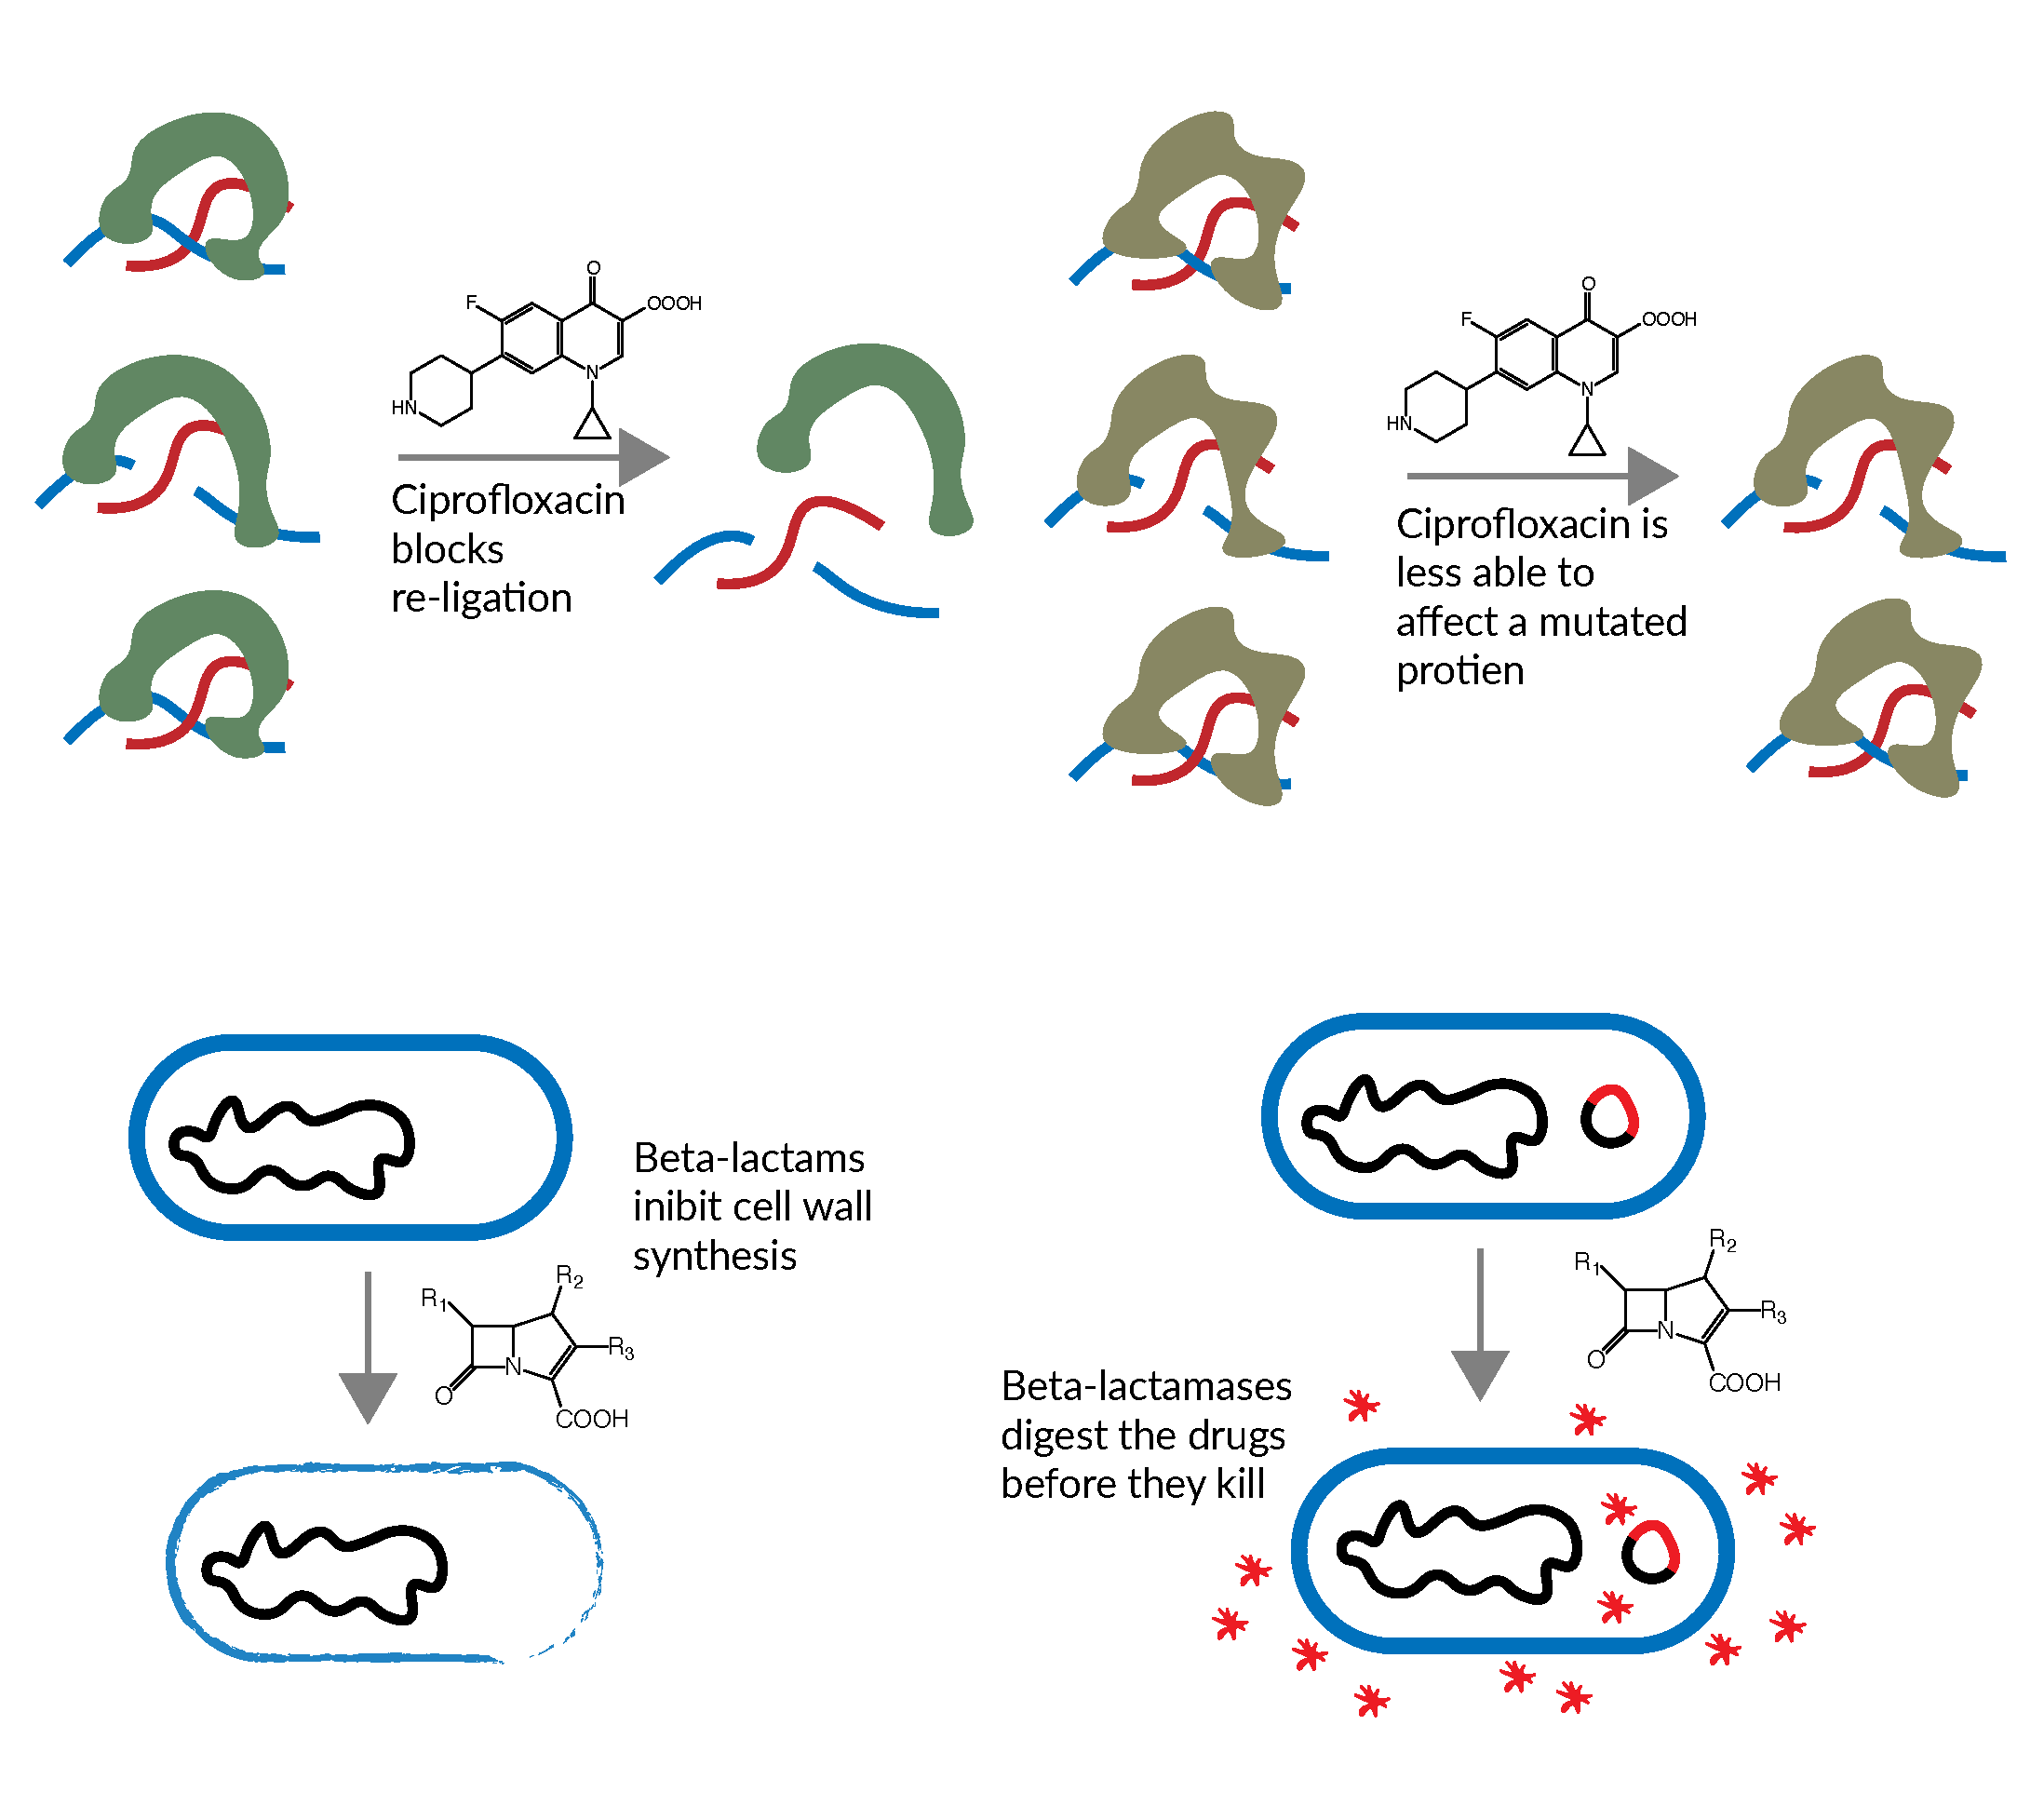
\includegraphics[width = .81\linewidth,keepaspectratio]{figure/rescartoons.pdf}
\caption[Resistance mechanisms]{{\bf Resistance mechanisms.} Drug resistances can arise through acquisition of a protective gene, such a {\textbeta}-lactamase gene. Mutations to a drug target such as the \textit{gyrA} topoisomerase gene can also reduce the effectiveness of antimicrobial agents. }
\label{fig:rescartoons}
\end{figure}


\begin{figure}[!ht]
\centering
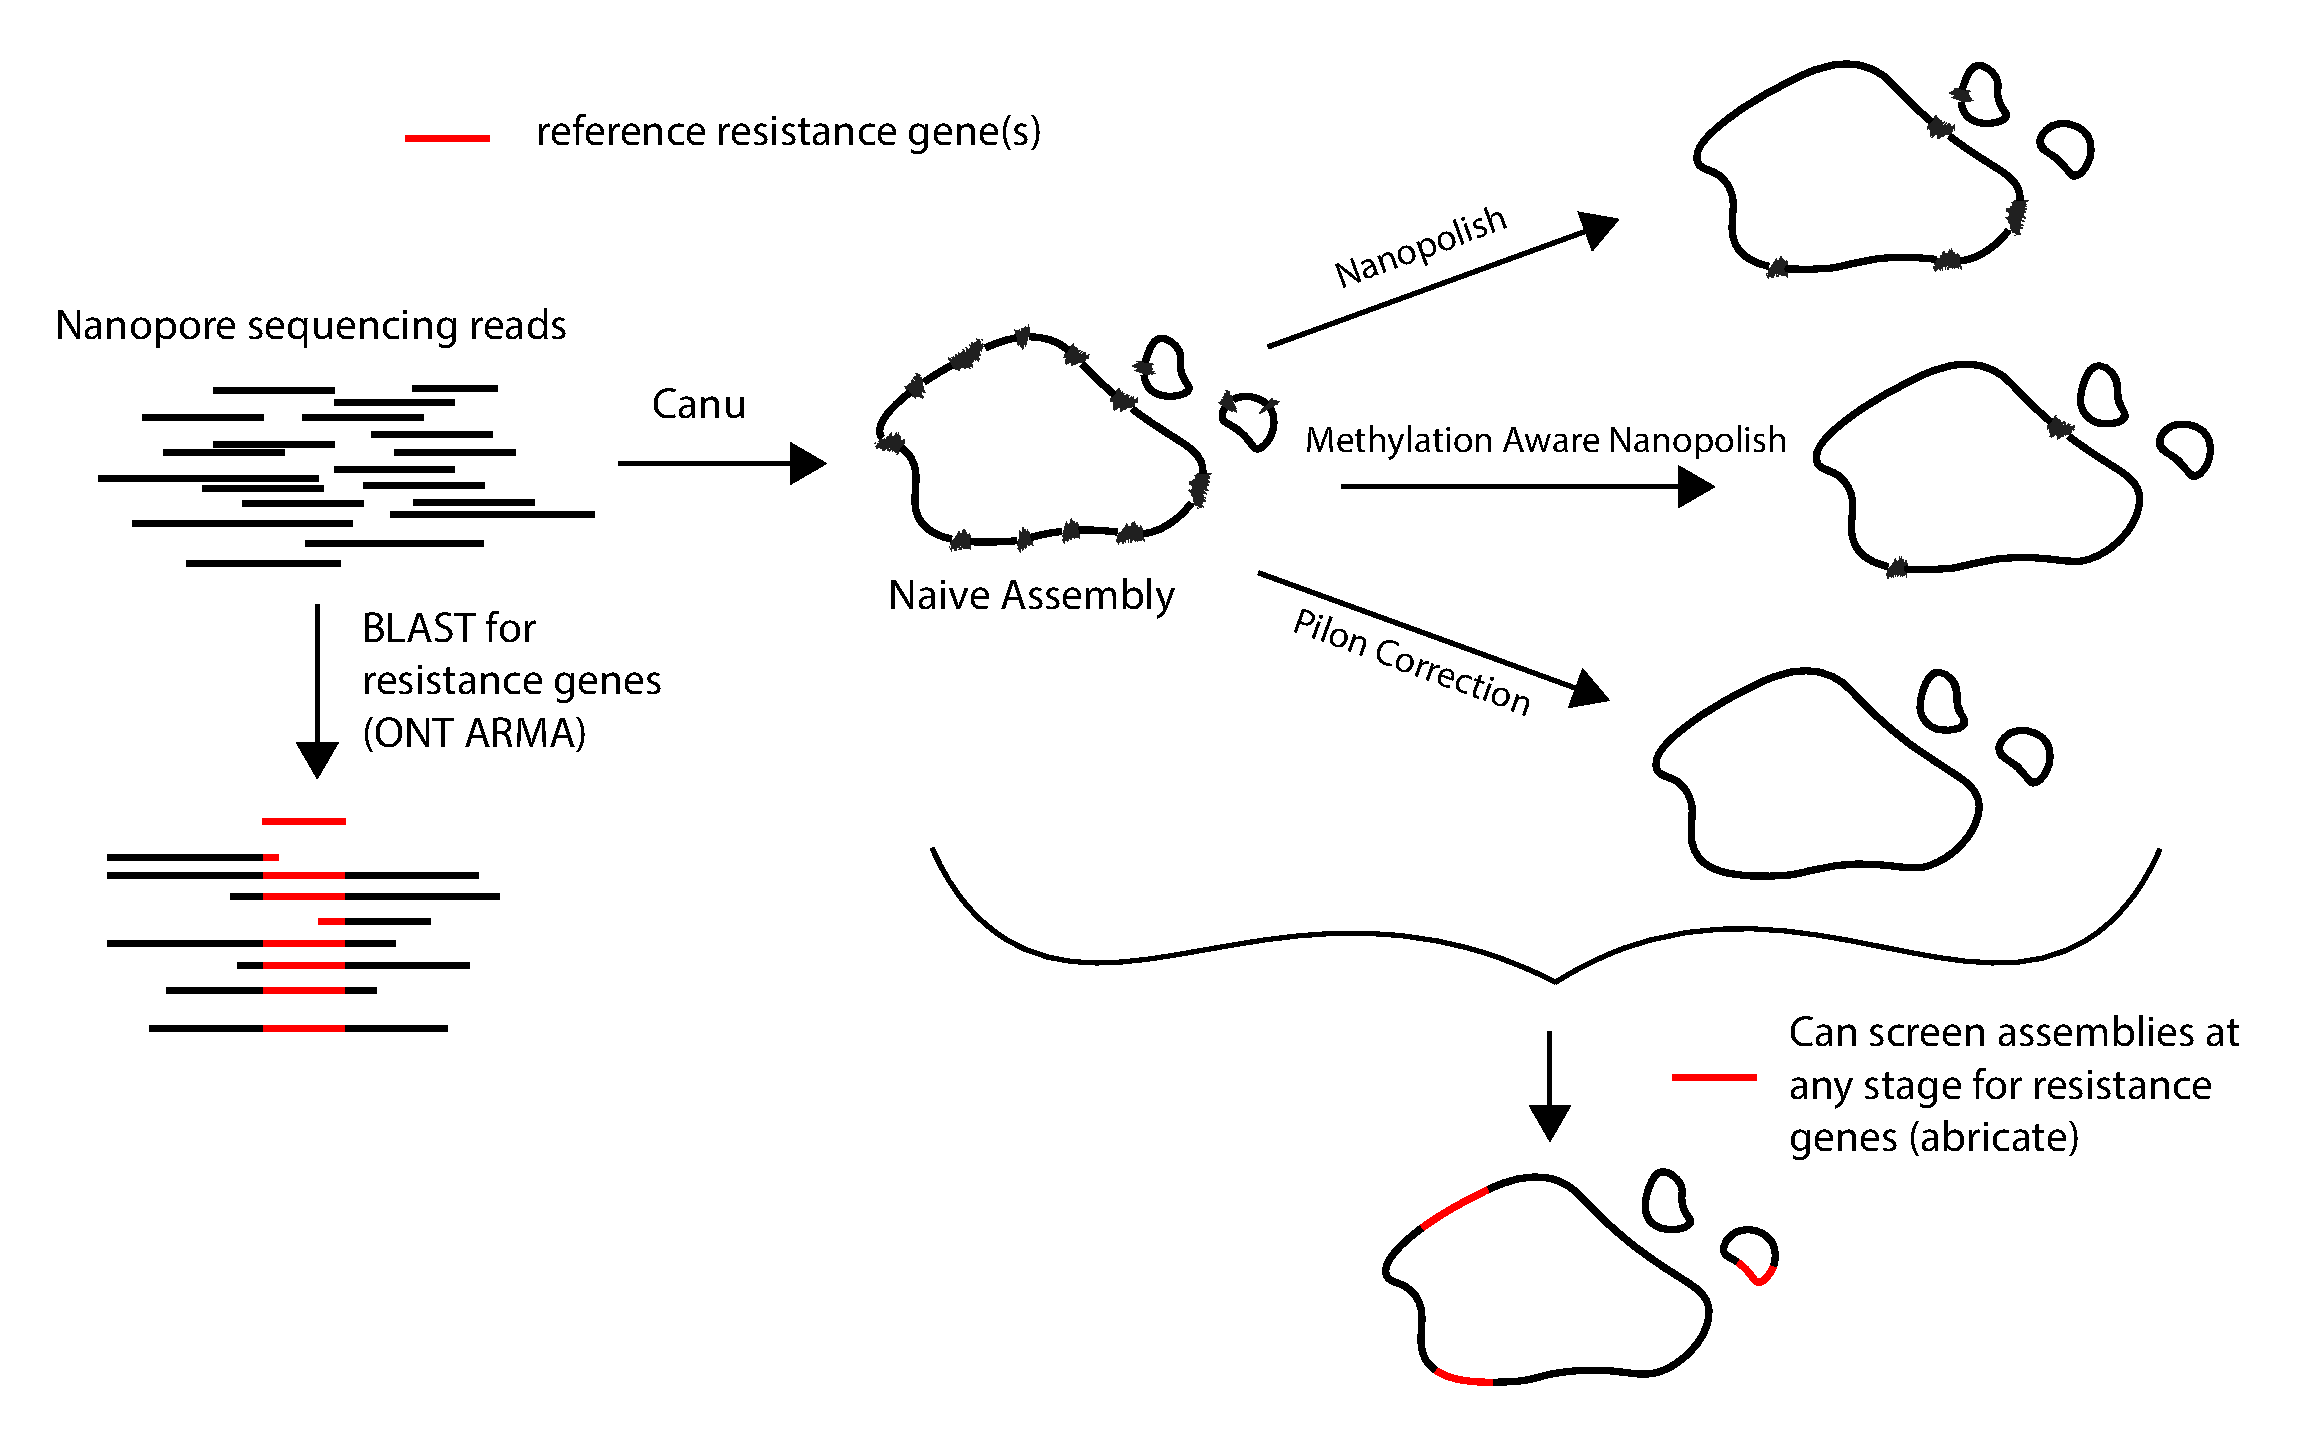
\includegraphics[width = 1\linewidth,keepaspectratio]{figure/pipeline.pdf}
\caption[Sequencing analysis pipeline]{{\bf Sequencing analysis pipeline.} Sequencing reads can be searched in real-time for resistance genes. To detect and assess point mutations, genomes are assembled, and then can be polished using native electrical data (Nanopolish), or highly accurate short-read data (Pilon). }
\label{fig:pipeline}
\end{figure}


\begin{figure}[!ht]
\centering
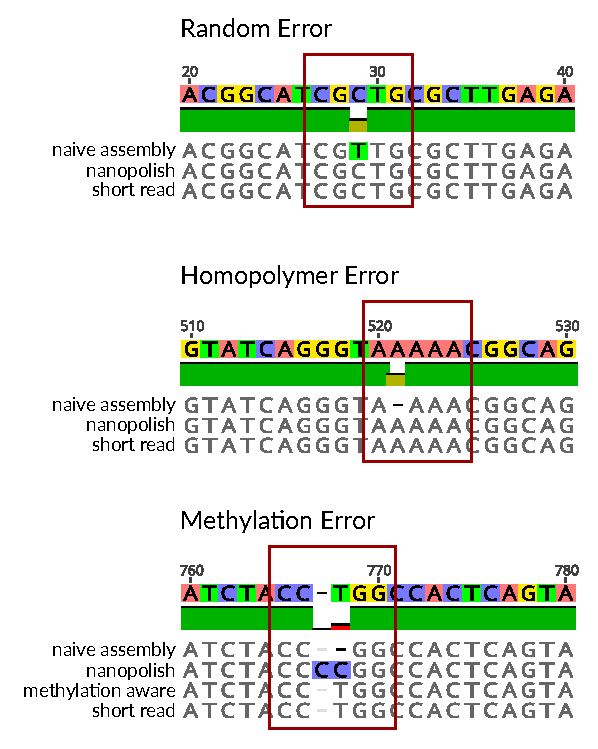
\includegraphics[width = .75\linewidth,keepaspectratio]{figure/npfixes.pdf}
\caption[Correction examples]{{\bf Correction examples.} Nanopolish corrects most random errors which persist after genome assembly to agree with short-read correction. It also corrects homopolymer errors, the most prominent systematic error on the ONT platform. Methylation-associated errors, such as those in the context of the dcm methyltransferase (CCWGG), are more effectively corrected using the methylation-aware mode. }
\label{fig:npfixes}
\end{figure}



\section{Results}
\label{sec:results}

\subsection{Sequencing runs and genome assemblies}
\label{sec:runs}

The nanopore sequencing runs yielded a mean of 6.4Gbp of sequencing data ({\bf Table \ref{tab:runnanopore}}), with all but one yielding at least 1 Gbp. As the \textit{Klebsiella pneumoniae} genome is only 5Mbp, this mean yield accounts for a greater than 1000X sequence coverage per isolate. Illumina sequencing runs yielded an average of 201Mbp per run ({\bf Table \ref{tab:runillumina}}), resulting in an average of 40X coverage. Using the regular assembly pipeline, 38 of the 40 genome assemblies appear to contain a full length bacterial chromosome at least 5Mbp long ({\bf Figure \ref{fig:graphsasm}, Table \ref{tab:asmraw}}). Further polishing steps both with and without Illumina data do not significantly affect the contig lengths in the assemblies ({\bf Tables \ref{tab:asmpolished}, \ref{tab:asmpilon}}). With the rapid analysis pipeline using downsampled data, 35 of the 40 assemblies contain a chromosome length contig ({\bf Table \ref{tab:asmrapid}}). Using the illumina-corrected assemblies, we were able to place our isolates in the context of other previously published, chromosome-level assemblies available in GenBank ({\bf Figure \ref{fig:tree}}).

\begin{table}[!ht]
\centering
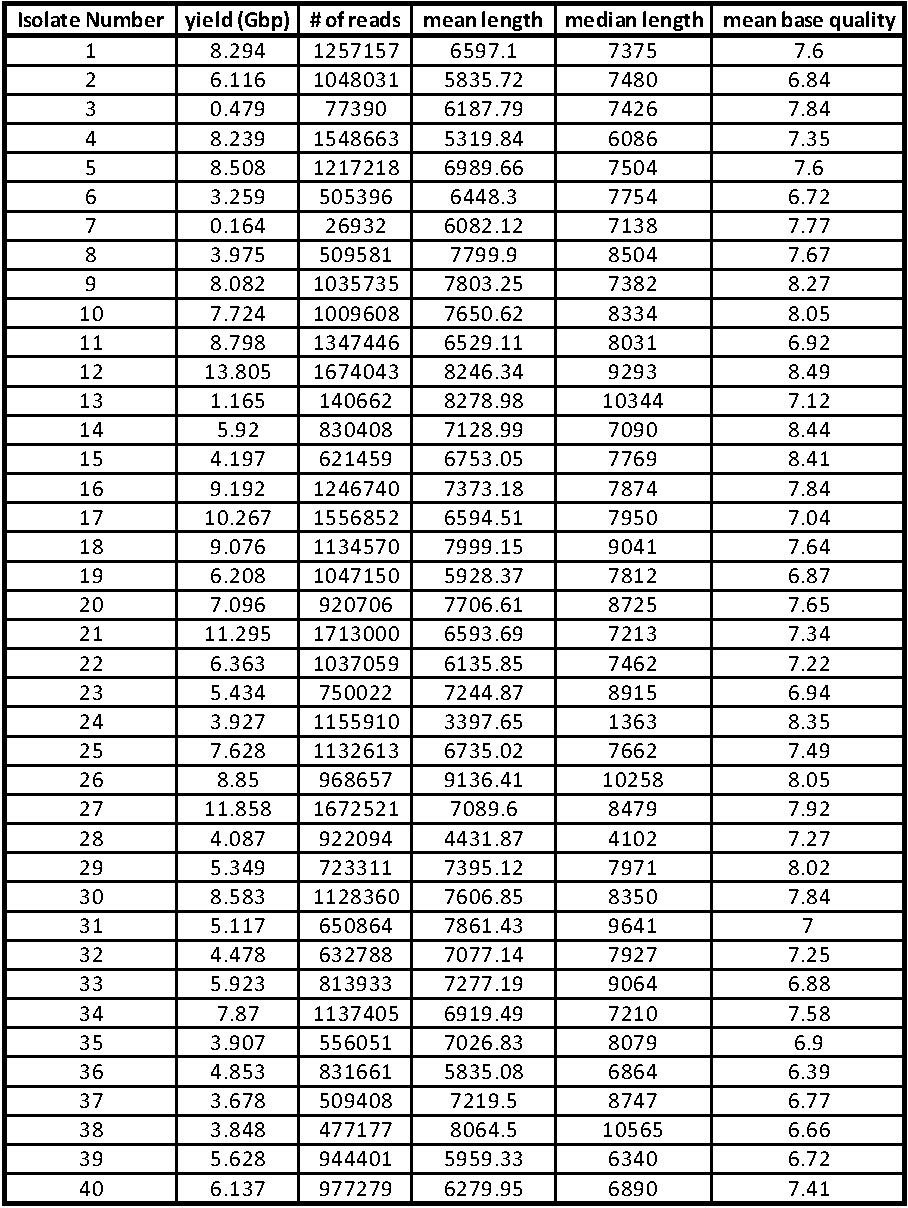
\includegraphics[width = .7\linewidth,keepaspectratio]{figure/runnanopore.pdf}
\caption[Nanopore sequencing data]{{\bf Nanopore sequencing data.} Summary of nanopore sequencing data for each isolate }
\label{tab:runnanopore}
\end{table}


\begin{table}[!ht]
\centering
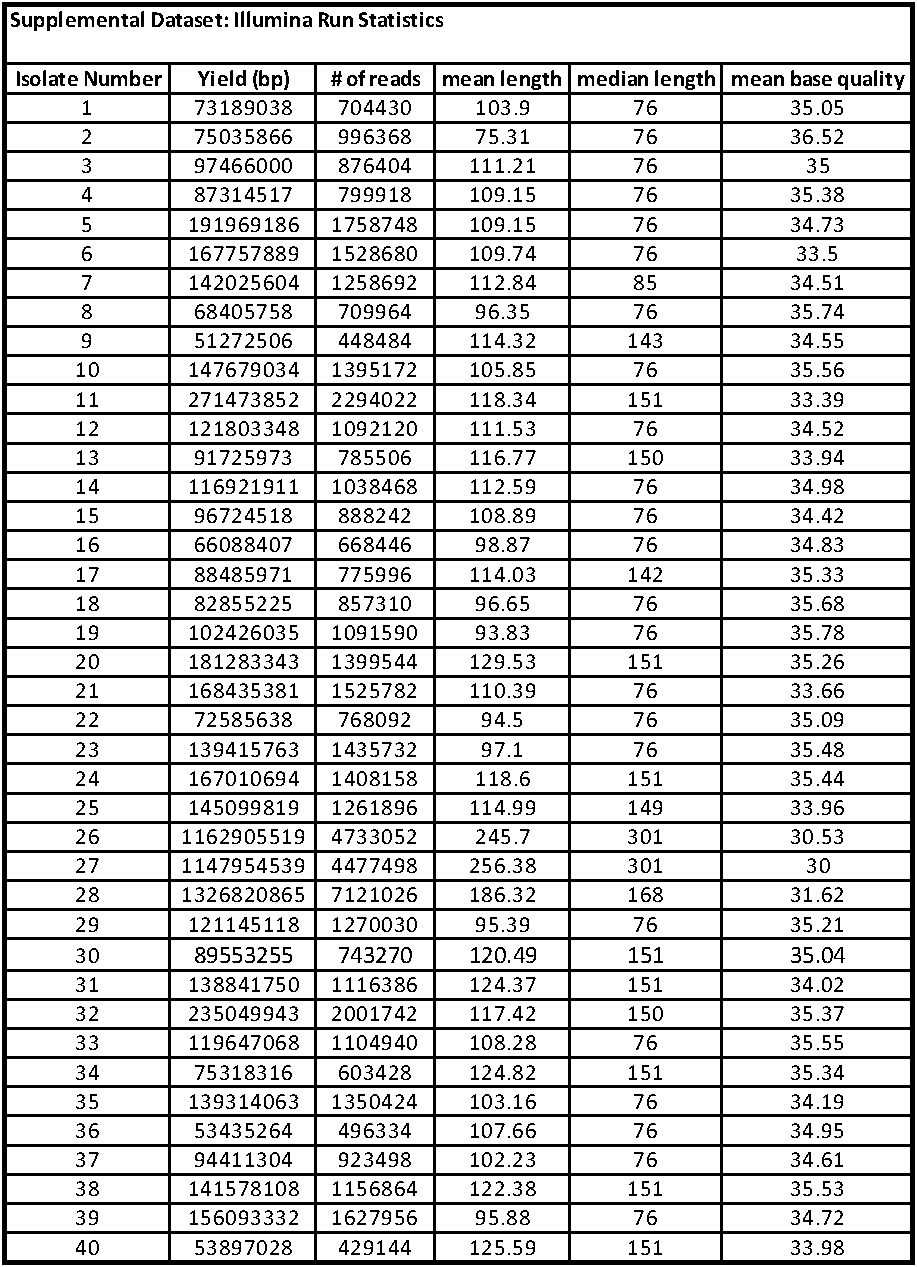
\includegraphics[width = .7\linewidth,keepaspectratio]{figure/runillumina.pdf}
\caption[Illumina sequencing data]{{\bf Illumina sequencing data.} Summary of Illumina sequencing data for each isolate }
\label{tab:runillumina}
\end{table}


\begin{figure}[!ht]
\centering
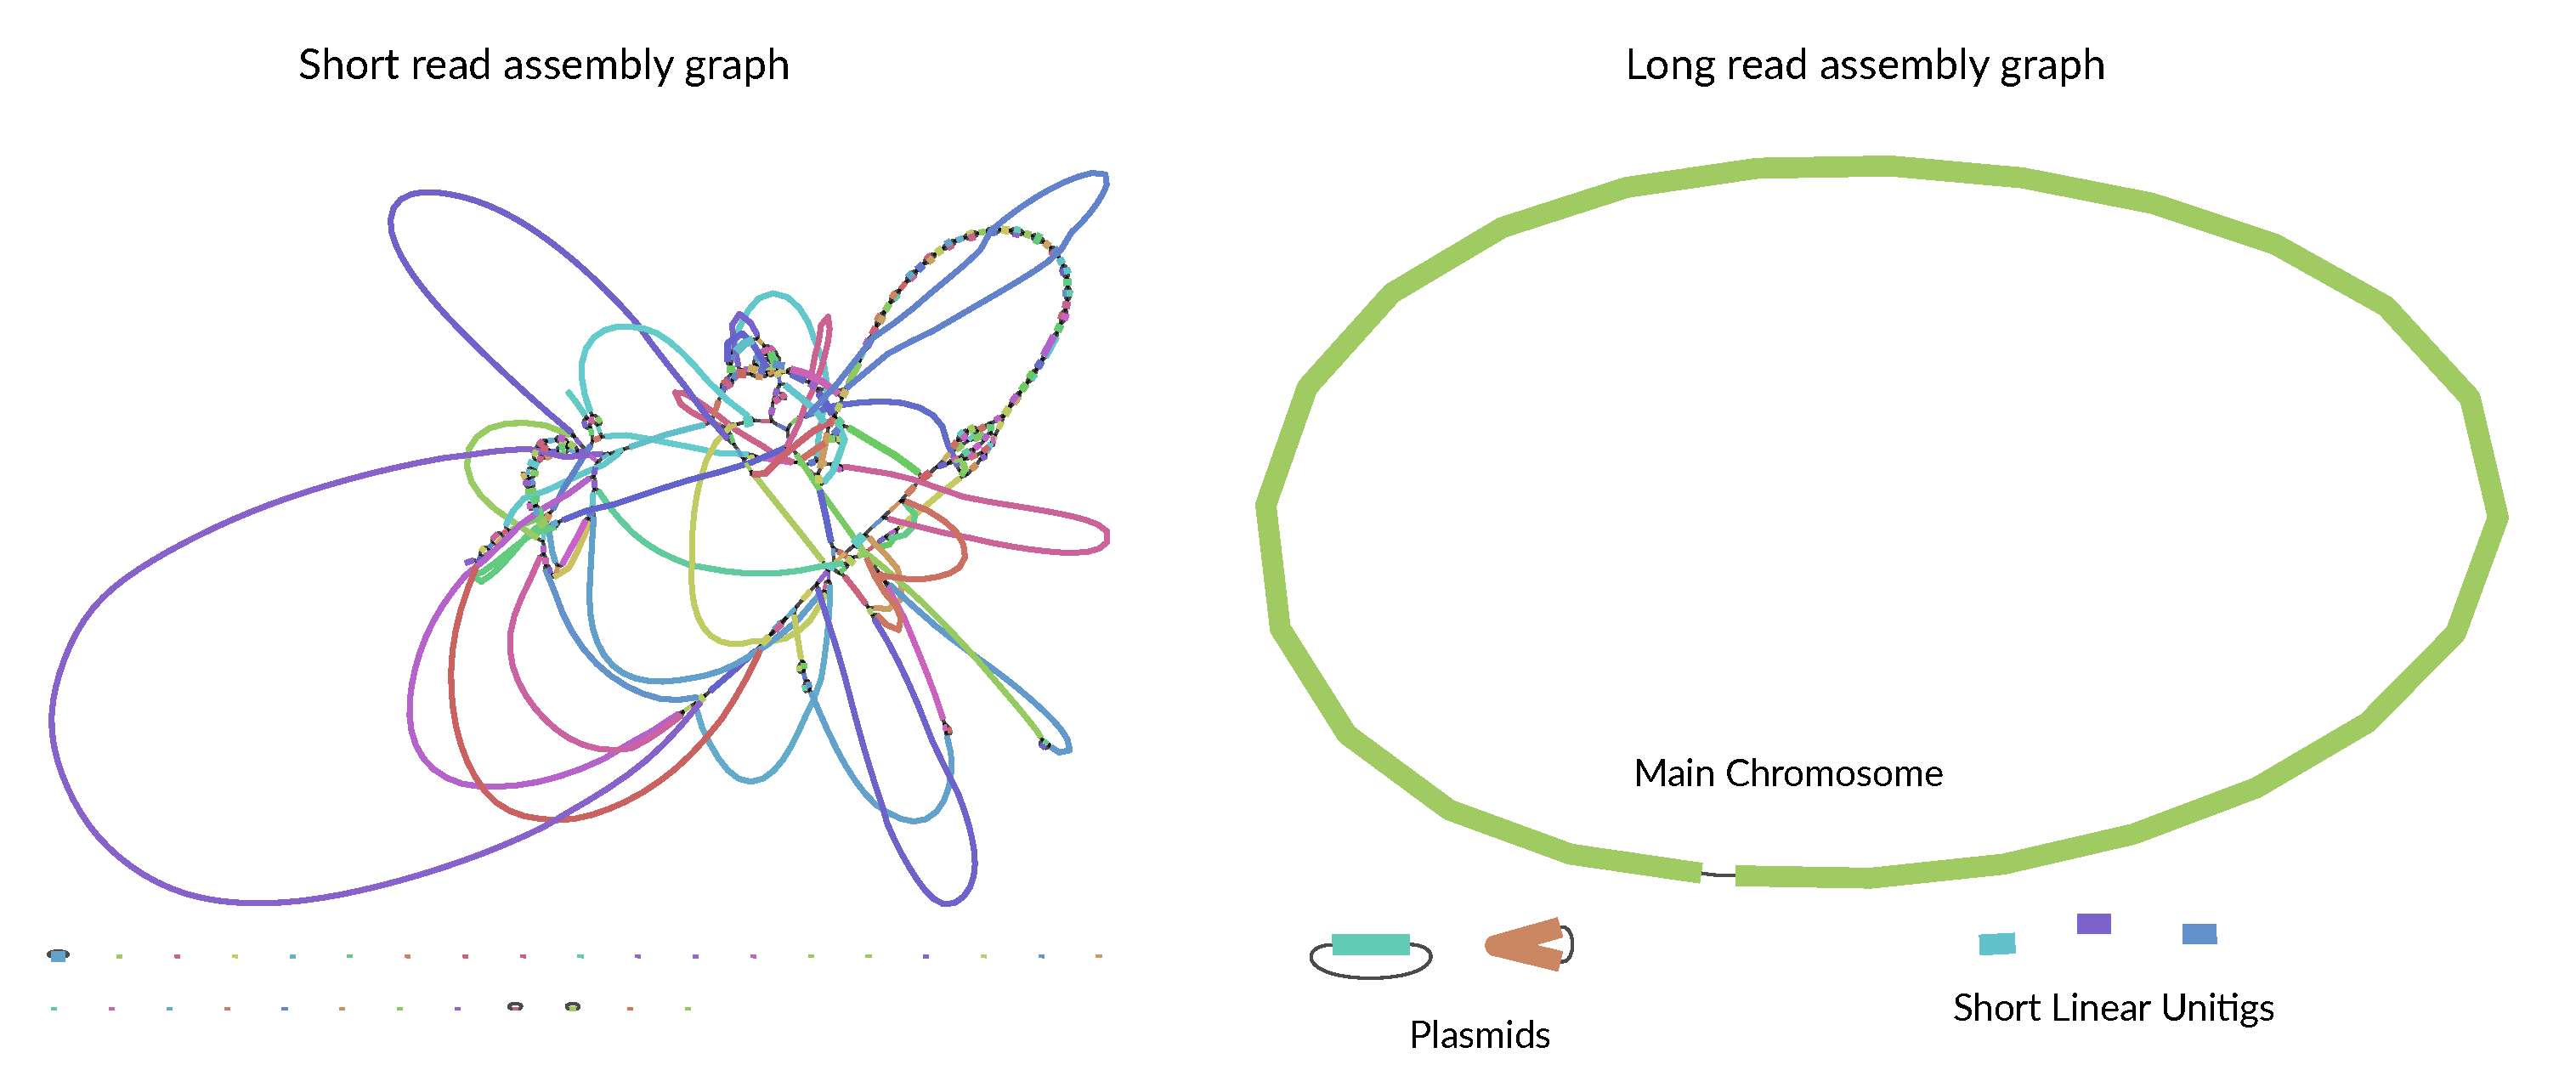
\includegraphics[width = 1\linewidth,keepaspectratio]{figure/graphsasm.pdf}
\caption[Assembly graphs]{{\bf Assembly graphs.} Representative assembly graphs when using only short reads and only long reads. Short reads are difficult to use for resolving repetitive regions, resulting in bubbles in the graph, whereas assemblies from long read data typically result in a full length bacterial chromosome. }
\label{fig:graphsasm}
\end{figure}


\begin{table}[!ht]
\centering
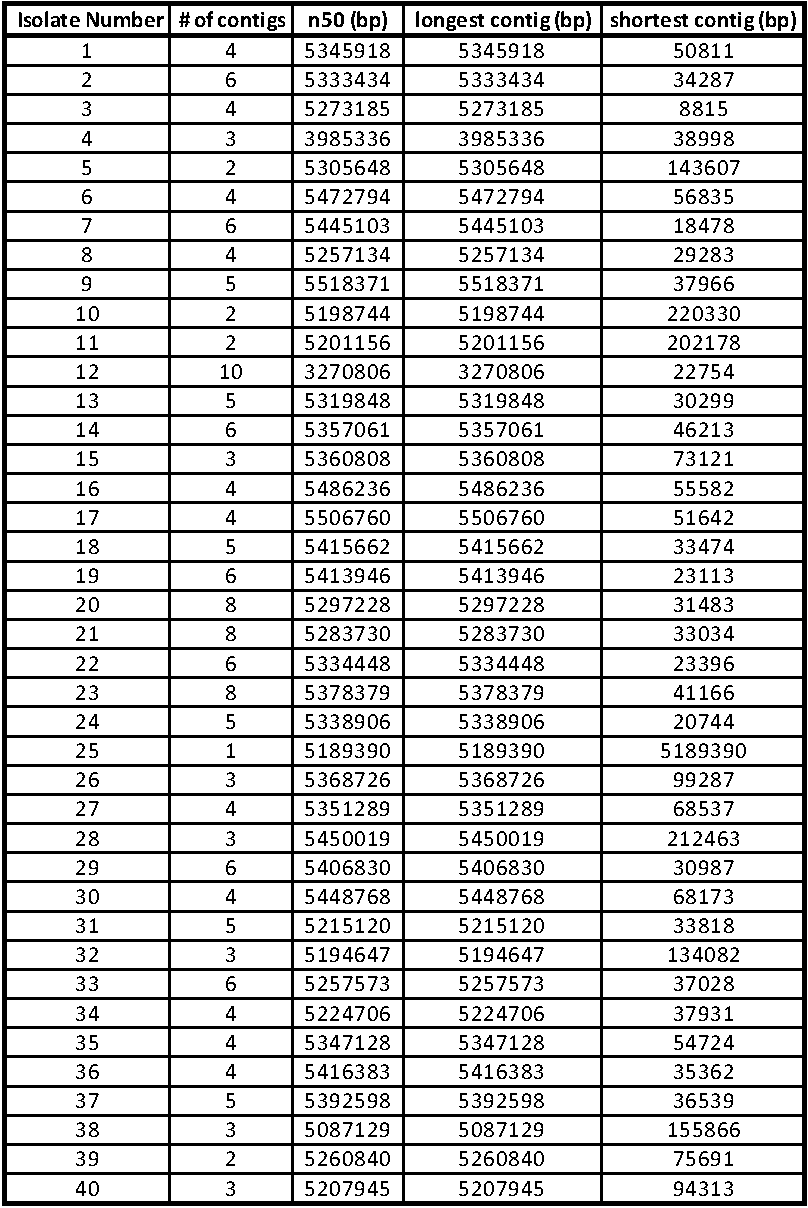
\includegraphics[width = .7\linewidth,keepaspectratio]{figure/asmraw.pdf}
\caption[Raw assembly statistics]{{\bf Raw assembly statistics.} Summary statistics for genome assemblies of all isolates with no further correction }
\label{tab:asmraw}
\end{table}


\begin{table}[!ht]
\centering
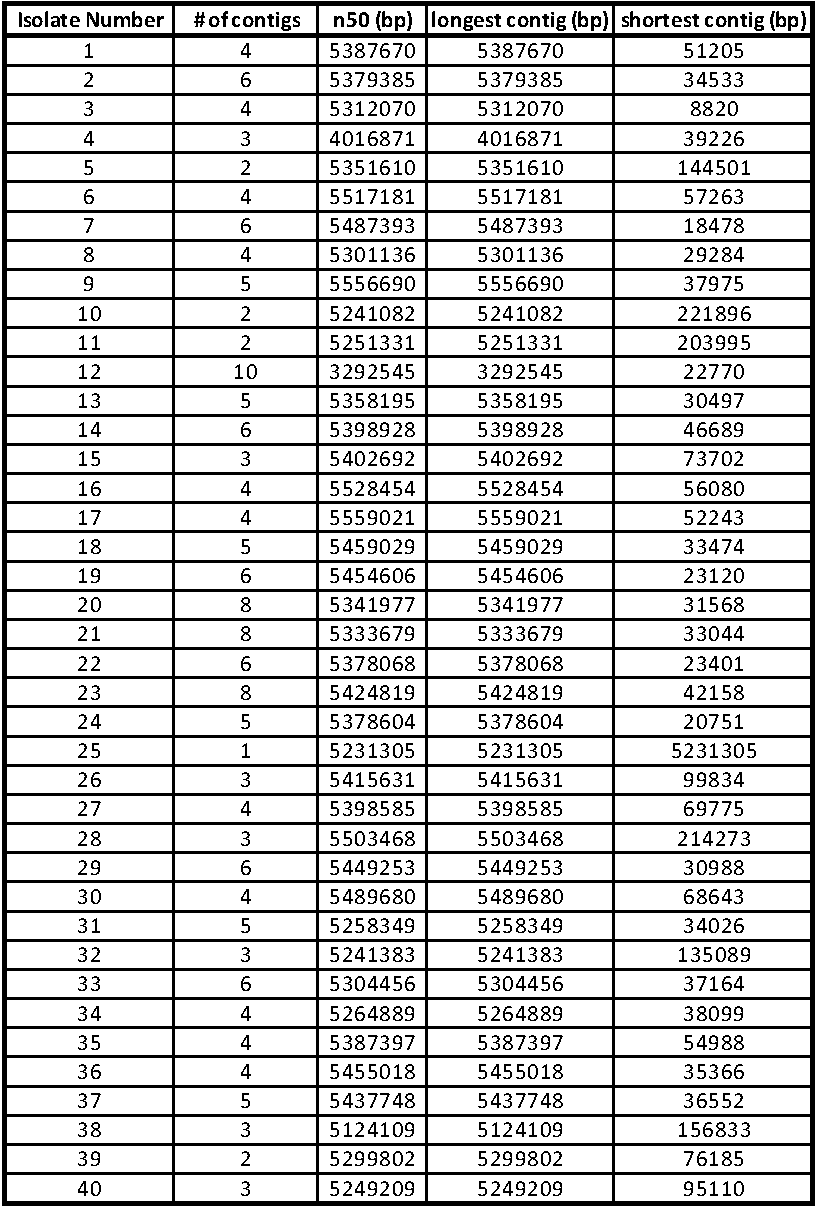
\includegraphics[width = .7\linewidth,keepaspectratio]{figure/asmpolished.pdf}
\caption[Polished assembly statistics]{{\bf Polished assembly statistics.} Summary statistics for genome assemblies of all isolates after correction with nanopolish }
\label{tab:asmpolished}
\end{table}


\begin{table}[!ht]
\centering
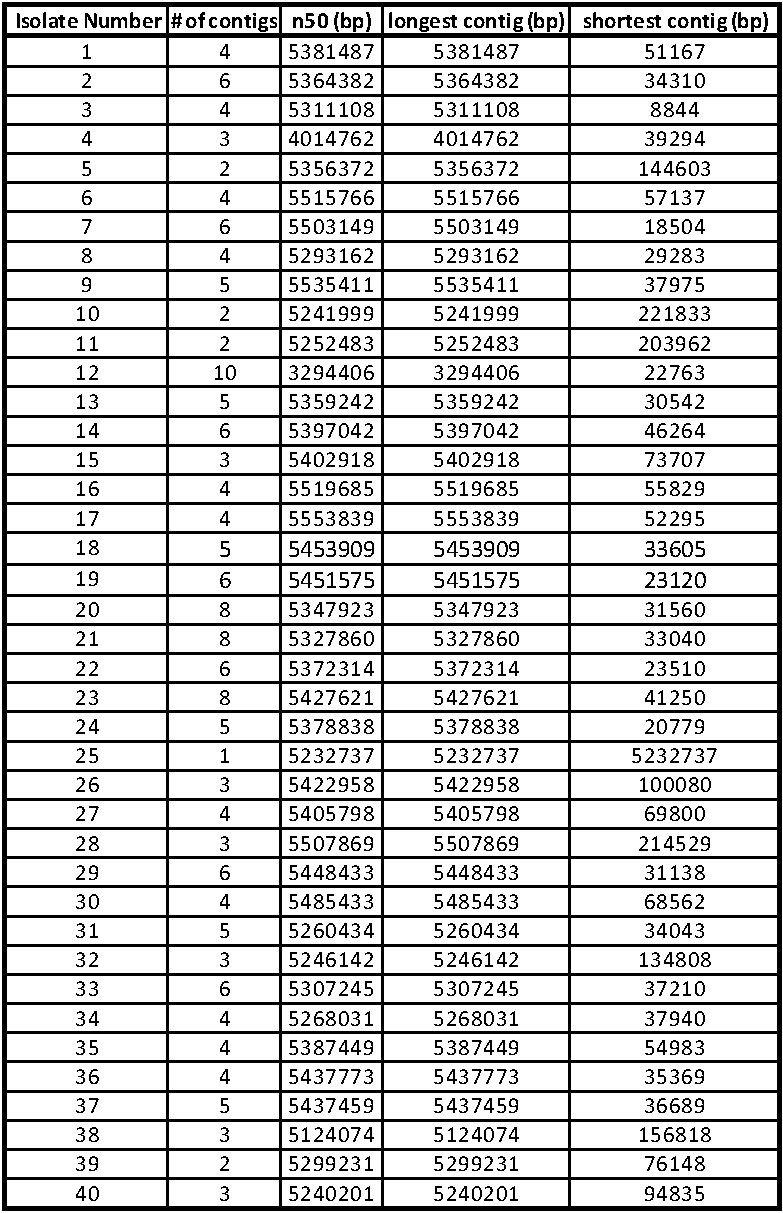
\includegraphics[width = .7\linewidth,keepaspectratio]{figure/asmpilon.pdf}
\caption[Short-read correction assembly statistics]{{\bf Short-read correction assembly statistics.} Summary statistics for genome assemblies of all isolates after correction with short-read data }
\label{tab:asmpilon}
\end{table}


\begin{table}[!ht]
\centering
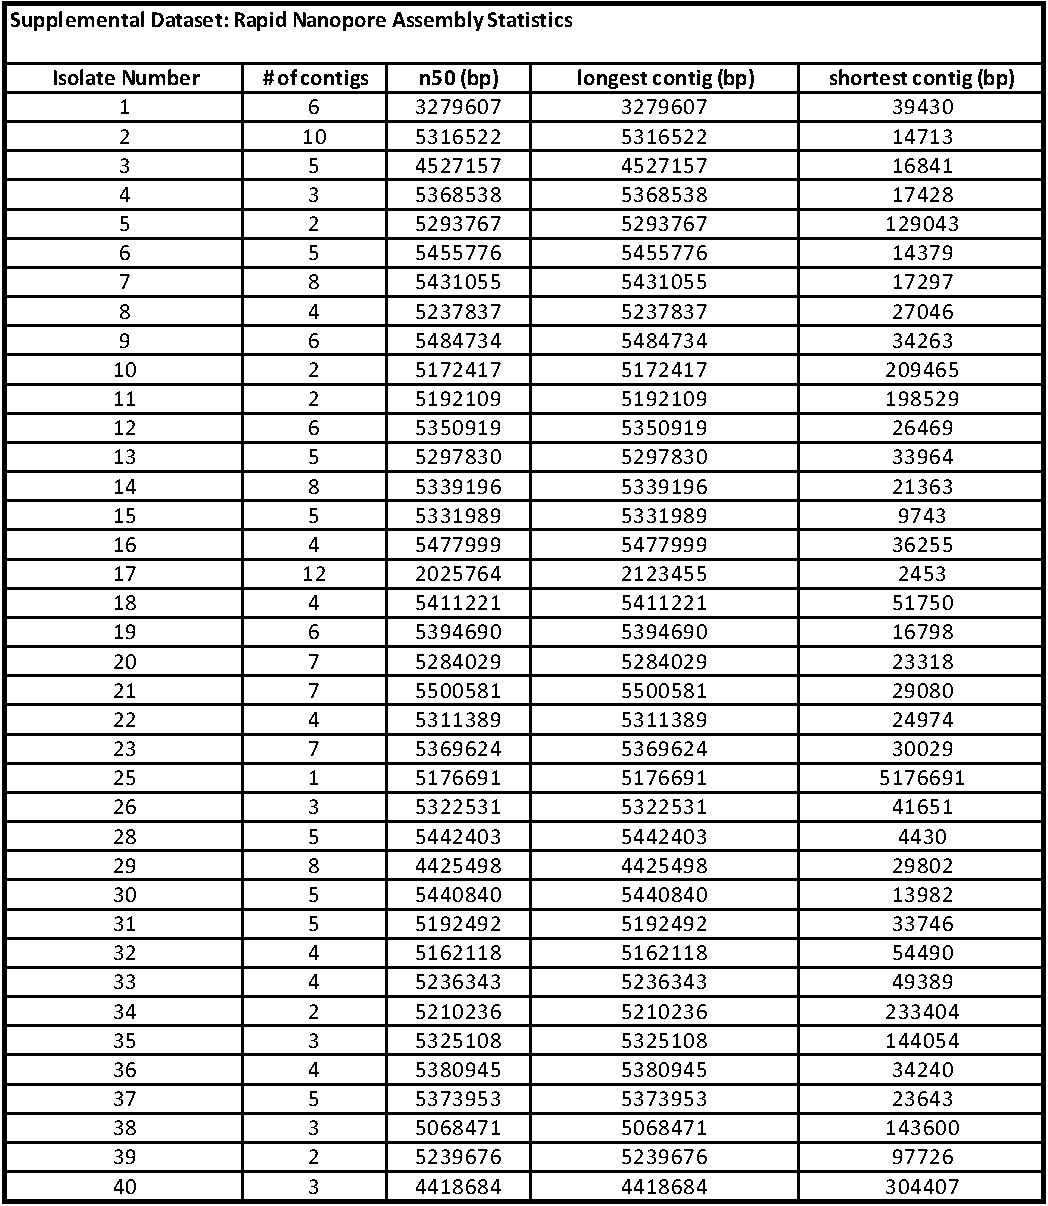
\includegraphics[width = .7\linewidth,keepaspectratio]{figure/asmrapid.pdf}
\caption[Rapid assembly statistics]{{\bf Rapid assembly statistics.} Summary statistics for genome assemblies of all isolates using downsampled data }
\label{tab:asmrapid}
\end{table}


\begin{figure}[!ht]
\centering
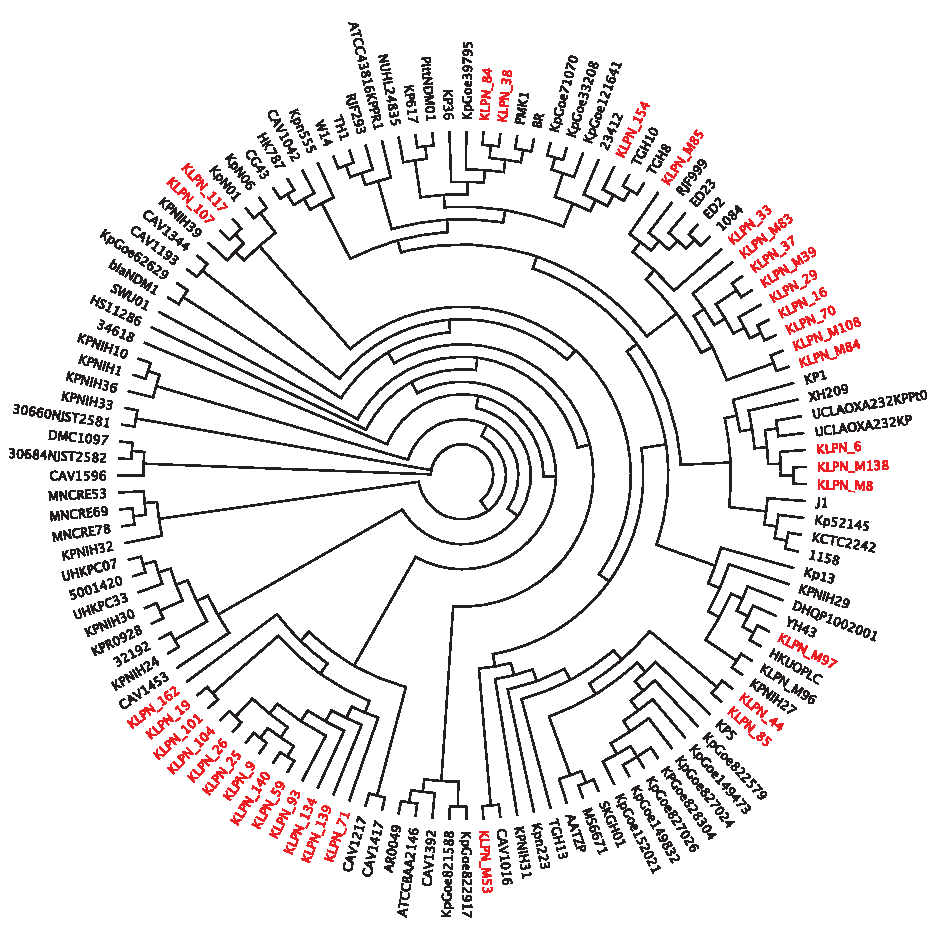
\includegraphics[width = .9\linewidth,keepaspectratio]{figure/tree.pdf}
\caption[Phylogenetic tree of \textit{K. pneumoniae} genomes]{{\bf Phylogenetic tree of \textit{K. pneumoniae} genomes.} Isolates from this study are shown in red, and chromosome-level genomes obtained from GenBank are shown in black. }
\label{fig:tree}
\end{figure}


\subsection{Percent agreement of WGS in predicting AST results}
\label{sec:agree}

The overall agreement of genotypic results and anticipated AST results for the 40  \textit{K. pneumoniae} isolates was 77\% (range, 30\% to 100\%), 92\% (range, 80\% to 100\%), and 92\% (range, 80\% to 100\%) for the Nanopore real-time approach, the Nanopore sequencing assembly approach, and the Pilon-corrected Illumina approach, respectively ({\bf Table \ref{tab:astagreement}}). The Nanopore real-time approach, compared to the assembly-based approach, had an inability to identify allelic variants (i.e., \textit{bla}\textsubscript{KPC} was identified but \textit{bla}\textsubscript{KPC-3} could not be specifically identified). Because all \textit{K. pneumoniae} isolates are known to have chromosomally integrated non-ESBL {\textbeta}-lactamase genes (e.g., \textit{bla}\textsubscript{SHV-1}, \textit{bla}\textsubscript{SHV-11}), when \textit{bla}\textsubscript{SHV} was identified, the assumption was that it was a non-ESBL \textit{bla}\textsubscript{SHV}. This led to reductions in the accuracy of predictions for several {\textbeta}-lactams, including 5\%, 2\%, and 3\% reductions in accurate predictions for piperacillin-tazobactam, ceftriaxone, and cefepime, respectively. Also, since the number of aminoglycoside-modifying enzymes were important to predict aminoglycoside resistance, and the alleles could not be distinguished, this led to decreases in accurate predictions for amikacin (reduced by 7\%) and gentamicin (reduced by 48\%). Additionally, the real-time approach was unable to identify chromosomal mutations, leading to decreases in accurate predictions for ciprofloxacin/levofloxacin (reduced by 68\%) and colistin (reduced by 5\%).

\begin{table}[!ht]
\centering
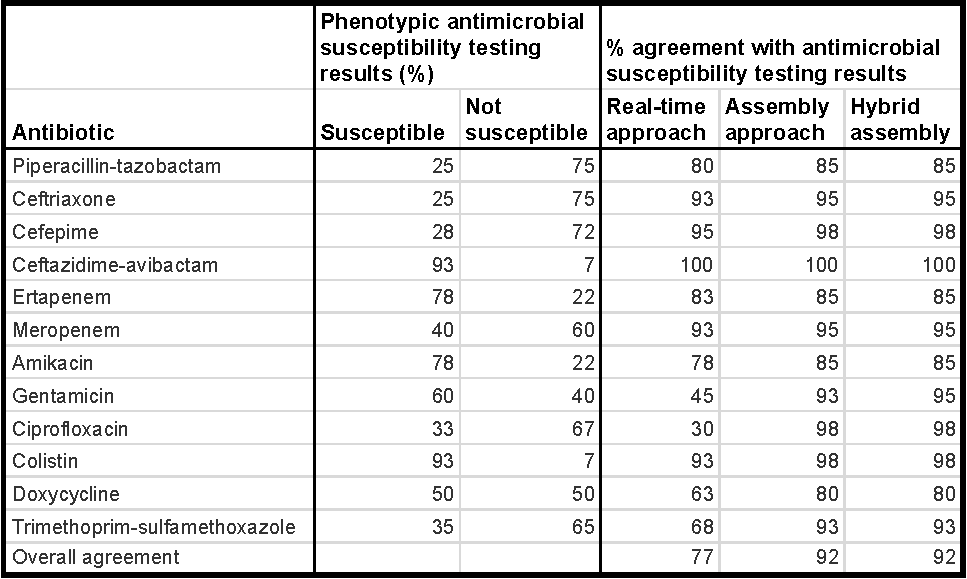
\includegraphics[width = 1\linewidth,keepaspectratio]{figure/astagreement.pdf}
\caption[WGS vs phenotypic AST]{{\bf WGS vs phenotypic AST.} Percent agreement between three different sequencing and analysis approaches compared to phenotypic antimicrobial susceptibility testing results for 40 \textit{Klebsiella pneumoniae} clinical isolates }
\label{tab:astagreement}
\end{table}


\subsection{Time to resistance determination}
\label{sec:time}

With a Nanopore real-time analysis approach, acquired resistance genes were identified within 8 h from subcultured isolates. Assemblies sufficient for full resistance gene and single-nucleotide polymorphism annotation using Nanopore sequences (Nanopore assembly approach) were available within 14 h from subcultured isolates. {\bf Figure \ref{fig:timeline}} compares the Nanopore real-time analysis and assembly approaches with standard-of-care methods. {\bf Table \ref{tab:astagreement}} summarizes the agreements between antibiotic resistance determinants identified using the real-time approach, assembly-based approach, or hybrid Nanopore-Illumina assemblies and AST predictions.

\begin{figure}[!ht]
\centering
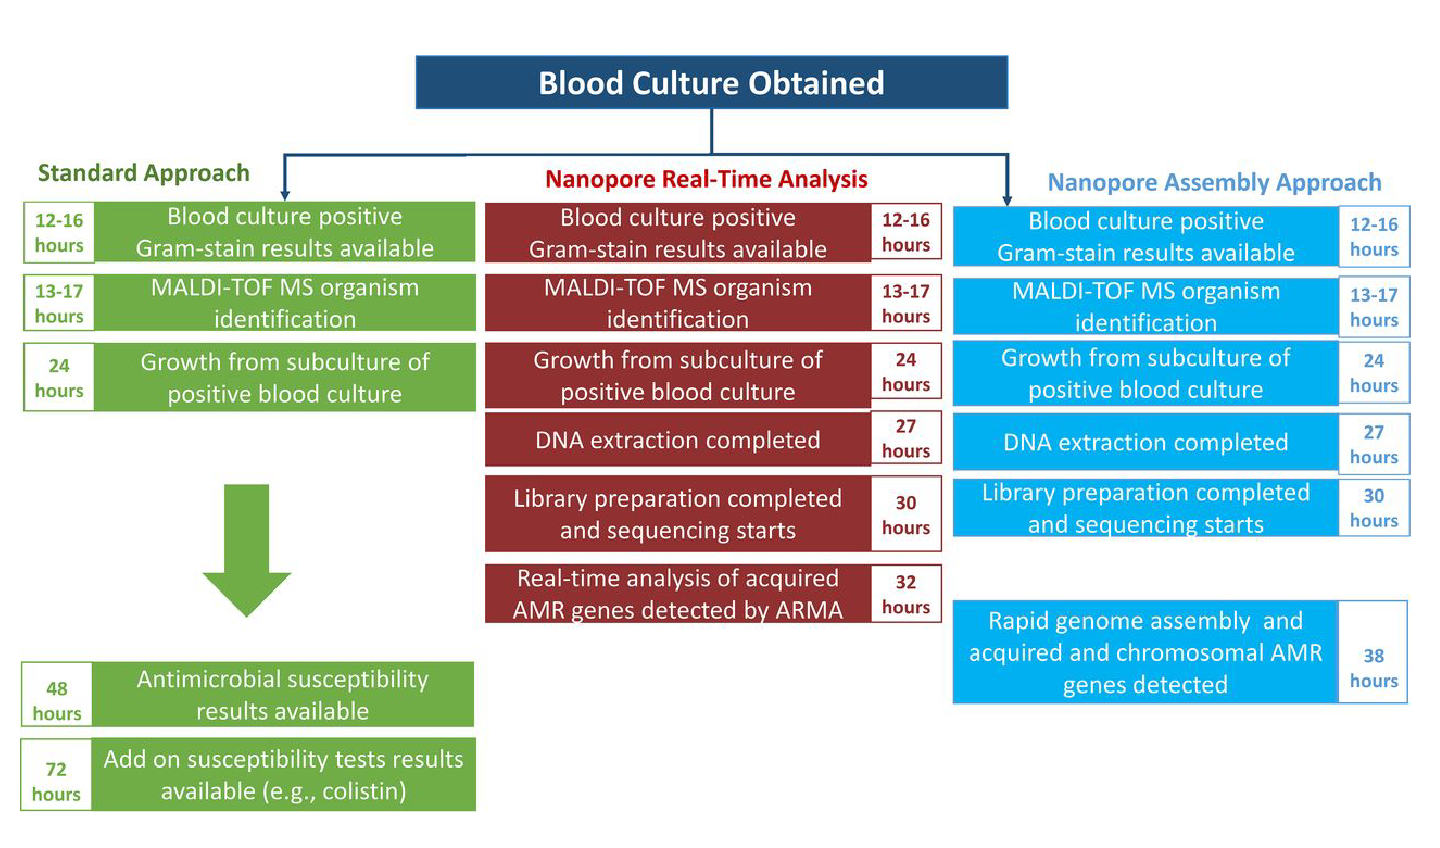
\includegraphics[width = 1\linewidth,keepaspectratio]{figure/timeline.pdf}
\caption[Estimated timelines of resistance detection]{{\bf Estimated timelines of resistance detection.} Schematic of Nanopore sequencing with a real-time analysis and assembly-based approach for identifying resistance genes compared to standard of care testing, using an example of a positive blood culture. MALDI-TOF MS, matrix-assisted laser desorption ionization<U+2013>time of flight mass spectrometry; AMR, antimicrobial resistance; AST, antimicrobial susceptibility testing. }
\label{fig:timeline}
\end{figure}


There were 28 patients in the cohort infected with carbapenem-resistant \textit{K. pneumoniae} strains. Overall, 22 (79\%) received empirical antibiotic therapy that was not active against their infecting isolates. Results from Nanopore sequencing with assembly approach had the potential to place 20 (91\%) of these patients on effective therapy sooner than did standard AST methods.

Overall, the median time to effective antibiotic therapy for the 28 patients infected with carbapenem-resistant \textit{K. pneumoniae} was 61 h (interquartile range [IQR], 43 to 82 h). Of the antibiotics evaluated, ceftazidime-avibactam, extended-infusion meropenem, aminoglycosides, fluoroquinolones, polymixins, and tigecycline are generally considered reasonable treatment options for infections caused by carbapenem-resistant \textit{K. pneumoniae} isolates, if active in vitro. As results from the real-time analysis approach were generally available within 8 h from subcultured isolates, Nanopore real-time analysis could have led to an average time to effective therapy of 41 h (IQR, 33 to 44). Using the Nanopore assembly approach, time to effective therapy could have been reduced to 35 h (IQR, 32 to 42). The time to effective therapy was reduced with the assembly approach compared to that with the real-time approach because the former provided more comprehensive data to infer AST activity (e.g., aminoglycoside resistance, colistin resistance, etc.) than the real-time approach, for which there were delays in antibiotic optimization while awaiting additional AST results. Both the real-time and assembly approaches were significantly faster than the standard approach.


\section{Discussion}
\label{sec:discuss}

Our results demonstrate that Nanopore sequencing can be employed to both accurately and rapidly predict phenotypic AST profiles. Our study builds off previously published proof-of-concept or early insight studies applying Nanopore sequencing for the detection of antimicrobial resistance genes \citep{Judge2015-zw, Judge2016-ds, Li2019-op, Van_der_Helm2017-ww, Xia2017-ss, Neuert2018-il, Hasman2014-el, Stoesser2013-se}. We found an overall agreement of 92\% between genotypic results and comprehensive AST results using a Nanopore assembly-based approach. We further demonstrated that assembly-based approaches enhance the ability to identify chromosomal mutations and allelic variants compared to that of the Nanopore real-time approach. A future method centered on real-time alignment and consensus of raw reads to a database of antimicrobial resistance (AMR) genes will enhance the capabilities of the real-time approach. Nevertheless, even with its current limitations, the Nanopore real-time analysis approach correctly predicted the presumed activity of a number of antibiotics commonly prescribed for Gram-negative infections, such as {\textbeta}-lactams, trimethoprim-sulfamethoxazole, tetracyclines, with reasonable accuracy, with full annotation of acquired AMR genes within 8 h from the time of cultured isolates. Within 14 h of cultured isolates, a Nanopolished assembly-based approach would allow for predictions of the activity of additional agents, such as fluoroquinolones, aminoglycosides, and polymixins (beyond \textit{mcr}-1 and its variants), due to the ability to detect chromosomal mutations or allelic variants leading to resistance. We believe that with rapid extraction and library preparation techniques, the turn-around times could further be reduced to 	{\textless}3 h for a real-time approach and {\textless}9 h for a Nanopore assembly-based approach. Moreover, using a hypothetical trial design, we found that a real-time approach and assembly approach could shorten the average time to effective antibiotic therapy for carbapenem-resistant \textit{K. pneumoniae} infections by 20 h and 26 h, respectively, compared to standard approaches.

Although there have been other investigations of the use of WGS to predict AST results for Gram-negative organisms based on resistance determinants \citep{Shelburne2017-dm, Cao2016-oj, Schmidt2017-ng, Lemon2017-td, Judge2015-zw, Judge2016-ds, Li2019-op, Van_der_Helm2017-ww, Xia2017-ss, Stoesser2013-se}, ours is the first to use a Nanopore assembly approach for evaluating a broad range of acquired resistance genes and chromosomal mutations in predicting susceptibility results for a comprehensive panel of antibiotics. Previous studies applying Nanopore sequencing for resistance gene detection have applied this methodology to small numbers of isolates and limited evaluations to acquired resistance genes. Furthermore, the potential impact of WGS in reducing time to appropriate antibiotic therapy for highly drug-resistant organisms has not been previously reported. As the science of WGS continues to evolve, the costs of sequencing are becoming more affordable, and the time requirements for DNA extraction, library preparation, assembly, and detection are anticipated to be further reduced. We believe that this methodology can accurately expedite antibiotic decision making for critically ill patients infected with MDRGN organisms. WGS also provides the ability to identify emerging mechanisms of resistance, such as \textit{mcr} variants or novel mechanisms of resistance against newly approved agents \citep{Haidar2017-pk, Haidar2017-rw}.

As we continue to gain further insights into the complexities of resistance mechanisms present in Gram-negative organisms, it is becoming increasingly clear that sole reliance on the detection of {\textbeta}-lactamase genes to identify antibiotic resistance is insufficient. Such is the case with commercially available PCR-based methodologies (e.g., Cepheid Xpert Carba-R assay, BioFire FilmArray blood culture identification panel, Verigene Gram-negative blood culture test, etc.) that fail to identify the wide array of additional resistance determinants (e.g., porin deletions, multidrug efflux pumps, functioning of the two-component regulatory system, DNA gyrase mutations, off-panel targets, etc.). Using carbapenem-resistant \textit{K. pneumoniae} as a case study, over half of isolates render carbapenem antibiotics ineffective due to non-carbapenemase-mediated mechanisms \citep{Tamma2017-el}. Similarly, carbapenem resistance among \textit{Pseudomonas aeruginosa} strains in the United States is predominantly mediated by noncarbapenemase mechanisms, including the loss of OprD porin expression and/or upregulation of MexAB-OprM efflux pumps \citep{Lister2009-ex}. WGS offers a more comprehensive approach to identifying clinically relevant antibiotic resistance compared with standard PCR technologies.

Nanopore technology offers real-time DNA sequencing of long reads, which facilitate the process of high-quality genome assembly \citep{Lu2016-ru}. Additionally, they are better able to capture large regions of structural variation (e.g., insertions, deletions, duplications, translocations, inversions, etc.) and resolve repetitive regions accurately, compared to technologies which generate short-read data. However, there are some drawbacks to Nanopore sequencing \citep{Lu2016-ru}. Chromosomal mutations as small as single-base polymorphisms in DNA can result in drastic changes to proteins due to frame shifts or early truncations. Indels and resulting false positives in chromosomal mutations can be difficult to distinguish with Nanopore sequencing alone \citep{Jain2018-qp}. The assembly process generally removes random error, given sufficient sequencing coverage. However, systematic errors in the form of homopolymer indels and methylation errors still result in disagreement compared with Illumina-corrected assemblies. Nanopolish corrects most homopolymer indels, improving accuracy, but in its current form, it is not all-inclusive \citep{Loman2015-nf}. Methylation motifs alter the electrical signal from Nanopore sequencing, resulting in errors in base calling. We anticipate further improvements to the quality of Nanopore sequencing and available bioinformatics, enabling this technology to rapidly and accurately resolve variants of acquired resistance genes and characterize chromosomal mutations in the absence of assembly.

We assessed the minimum sequencing time to be able to accurately predict AST using Nanopore sequencing. We determined that a minimum of 10 reads per gene were required and that a sequencing run of 1 h is sufficient to predict the AST profile, using either a real-time sequencing workflow or an assembly approach. In fact, we were able to detect 10 reads of all AMR genes within 14 min of starting the sequencing run and 40 reads of each gene within 1 h. This is an important quality control measure as we begin to consider these methods for clinical application.

There are several remaining limitations to this work. First, there were some antimicrobial susceptibility profiles for which we were unable to identify the associated resistance mechanisms, suggesting that our approach to resistance detection was not comprehensive. As an example, we were only able to accurately predict piperacillin-tazobactam activity 85\% of the time. This is similar to what others have shown \citep{Shelburne2017-dm}, and it is likely due to efflux pumps, where expression analysis is required. Second, there were some agents tested for which no resistance was observed (e.g., tigecycline), precluding us from including these agents in our analysis. Third, we only evaluated \textit{K. pneumoniae} isolates from a single region of the United States. Validation needs to occur in larger data sets with a more diverse array of genera and species and resistance mechanisms, including some not observed in our isolates, such as the \textit{mcr} genes. Additionally, as antibiotic susceptibility criteria include several considerations, such as wild-type MIC distributions, pharmacokinetic-pharmacodynamic modeling, clinical outcomes data, etc., it can be challenging to determine the most accurate MIC that signifies nonsusceptibility. The European Committee on Antimicrobial Susceptibility Testing suggests that epidemiologic cutoff values (i.e., wild-type versus non-wild-type distributions) are the preferred values for correlation with resistance genes \citep{Eucast_undated-wa}. We elected to use antibiotic breakpoints, as these remain the most relevant metric for quantifying antibiotic resistance for clinicians, but we realize that this might not be the most accurate proxy.

In conclusion, we were able to leverage the long reads, rapid turnaround time, and real-time analytic capabilities of Nanopore sequencing to accurately identify resistance loci. With the continued rise in highly drug-resistant infections, the need for rapid and accurate methods to detect antibiotic resistance is becoming increasingly important. Continued enhancements to WGS may permit real-time AMR gene detection from clinical isolates in the near future.

\section{Materials and Methods}
\label{sec:methods}

\subsection{Study cohort}
\label{sec:cohort}

Forty clinical \textit{Klebsiella pneumoniae} complex isolates collected between 2016 and 2017 and processed at the Johns Hopkins Hospital Medical Microbiology Laboratory were included in the present study. Isolates for inclusion were deliberately selected based on their diversity of AST results and mechanisms of resistance and included 30 carbapenem-resistant (21 carbapenemase producers and 10 non-carbapenemase producers) and 9 carbapenem-susceptible \textit{K. pneumoniae} isolates. As this was a proof-of-concept study comparing different WGS approaches, we decided to focus on a single genus and species (i.e., \textit{K. pneumoniae}) to increase the number of isolates with any single resistance mechanism identified, as some resistance mechanisms are genus and species specific, especially among chromosomal mutations leading to resistance. Isolates were subcultured from frozen stock to tryptic soy agar (TSA) with 5\% blood agar. A second subculture was performed prior to DNA extraction. \textit{K. pneumoniae} isolates from deep tissue (n = 3), intraabdominal fluid (n = 1), blood (n = 10), respiratory (n = 10), and urine (n = 16) were included.

\subsection{Species and antimicrobial susceptibility testing}
\label{sec:ast}

Bacterial genus and species were identified using matrix-assisted laser desorption ionization–time of flight mass spectrometry (Bruker Daltonics Inc., Billerica, MA). AST results were determined using the BD Phoenix Automated System NMIC-303 panels (BD Diagnostics, Sparks, Maryland). MICs were confirmed by broth microdilution (BMD) with Sensititre GNX2F Gram-negative panels (Thermo Fisher Scientific, Indianapolis, IN) and the ceftazidime-avibactam Etest (bioMérieux, France) \citep{Matuschek2018-qh}. BMD was repeated on isolates with 2-fold or greater MIC discrepancies between the Phoenix automated panel and initial BMD results. Interpretive criteria established by the Clinical and Laboratory Standards Institute (CLSI) were used to define antibiotic susceptibility. AST results in both the “intermediate” and “resistant” ranges were categorized as resistant.

\subsection{Whole-genome sequencing and antimicrobial resistance gene detection}
\label{sec:wgs}

As Nanopore sequencing has a substantial raw sequencing error rate, three separate sequencing and analysis pipelines were performed, as follows: (i) a real-time Nanopore (Oxford, England) analysis approach that identified acquired and chromosomal resistance genes by applying Metrichor’s Antimicrobial Resistance Mapping Application (ARMA) (https://nanoporetech.com/resource-centre/real-time-detection-antibiotic-resistance-genes-using-oxford-nanopore-technologies); (ii) an assembly-based Nanopore approach that uses Canu and Nanopolish \citep{Loman2015-nf, Koren2017-wf} to compute high-identity sequences with identification of resistance genes, using Abricate ResFinder results as well as chromosomal mutations (e.g., ompK35 and ompK36 mutations, \textit{gyrA} and \textit{parC} mutations, etc.) from genomic assemblies, using minimap2 \citep{Li2018-eq} and a tool evaluating the impact on amino acid translation based on resulting codon changes (https://github.com/gpertea/pwasm); and (iii) a Pilon-corrected hybrid approach using both Illumina (Illumina, San Diego, California) and Nanopore sequencing \citep{Walker2014-eh}. The short-read correction of Nanopore assemblies served as the reference standard to determine the accuracy of Nanopore sequencing results.

Long-read genomic sequencing was performed using the third generation Oxford Nanopore MinION MkIb (Isolates 1-30) and GridION X5 (Isolates 31-40; Oxford, England) sequencing instruments. Genomic DNA was extracted from pure cultures using the DNeasy PowerBiofilm Kit (Qiagen, Hilden, Germany). Each Nanopore sequencing library was prepared using 5 µg of DNA with the 1D ligation kit (SQK-LSK108, Oxford Nanopore Technologies) using R9.4 flowcells (FLO-MIN106). A single isolate was run per flowcell. MinKNOW software was used to collect sequencing data.

For the real-time analysis approach, the Oxford Nanopore Technology “What’s In My Pot” (WIMP) \citep{Juul2015-zt} and Metrichor’s Antimicrobial Resistance Mapping Application (ARMA) real-time analysis tools were run in parallel to both sequencing and base-calling. WIMP uses a customized pipeline applying the Centrifuge metagenomic classifier to the sequencing reads. ARMA aligns sequencing reads to the Comprehensive Antimicrobial
Database (CARD) \citep{Jia2017-pg}, identifying antimicrobial resistance (AMR) gene hits.

For the assembly-based approach, Albacore v2.1.3 was used to base-call. Raw data were corrected, trimmed, and assembled using Canu v1.6 \citep{Koren2017-wf} using default parameters. Genome size was assumed to be 5.3Mb. For isolates that did not assemble under default parameters, either read quality restrictions were relaxed or minimum overlap requirements were shortened as suggested by the software documentation. Assembled contigs were screened for resistance genes using Abricate (https://github.com/tseemann/abricate), a tool that uses alignment to search for resistance gene sequences from several database including ResFinder, CARD, ARG-ANNOT, and the NCMI AMR Reference Gene Database. ResFinder results were evaluated in this study \citep{Zankari2012-uk}. In a separate experiment, we were able to build high quality genomes from nanopore electrical data in under 6 hours using a machine with 36 cores and 72GB RAM. Thirteen random blocks of 4000 reads were sampled and taken through basecalling, assembly and polishing. Conservatively, it takes at most an hour to reach 52,000 reads on a typical run.

WGS was also conducted using Illumina MiSeq short-read sequencing to increase assembly accuracy (Illumina, San Diego, California). A drawback with Illumina sequencing is the turn-around time as sequencing alone requires between 19-24 hours for 300 cycles. As the ultimate goal would be to use Nanopore sequencing alone for both resistance gene and chromosomal mutation identification, in the current analysis, the Pilon-corrected assemblies were not meant to supplant or supplement Nanopore sequencing but rather to serve as a reference standard to determine the accuracy of Nanopore sequencing results. Approximately 100-500 ng of gDNA was used to prepare sequencing libraries using the Nextera Flex Kit. The each Illumina library was then sequenced using both v2 2x150 and v3 2x75 reagents on an Illumina Miseq. These reads were used to correct the more error prone Nanopore assembly with the Pilon v1.22 software package in conjunction with the short-read aligner Bowtie2 v2.2.6. Phylogenetic trees were generated using Parsnp v1.2 \citep{Treangen2014-bu}.

\subsection{Predicted correlations between WGS and AST results}
\label{sec:wgsast}

Predictions of resistance were performed without reference to phenotypic data, unless otherwise noted in Results. The correlations of resistance genes and sequence variants with anticipated AST results for the evaluated antibiotics were determined based on reference gene databases and the published literature \citep{Bush2010-lg, Bush1995-rb, Jacoby2009-wr, Naas2008-vx, Evans2014-md, Zhang2014-xg, Feng-Jui2003-nf, Vetting2011-iu, Kim2009-me, Ramirez2010-sv, Galimand2012-gu, Liakopoulos2016-wl, Tarnberg2009-qg, Bonnet2004-xz, Roberts2005-js, Fevre2005-vm, Fu2013-cm, Poirel2010-ch}. Antimicrobial resistance genes and mutation results were reviewed manually to predict AST results. For associations for which ambiguity existed, the following rules were established a priori:
\begin{itemize}
  \item SHV 2be extended-spectrum {\textbeta}-lactamase enzymes were assumed to inactivate ceftriaxone and cefepime if they contained G238S or E240K mutations \citep{Liakopoulos2016-wl, Howard_Christopher2002-tr}
  \item The relative contributions of porins OmpK35 and/or OmpK36 truncations to {\textbeta}-lactam resistance have not been well established \citep{Zhang2014-xg, Shelburne2017-dm, Tsai2011-ly, Landman2009-gi, Jiang2009-hg, Domenech-Sanchez2003-fv}. There appears to be consensus that when premature stop codons are present for both, in conjunction with ESBLs or AmpC cephalosporinases, carbapenem resistance is likely.
  \item Aminoglycoside modifying enzymes (AMEs)- including aminoglycoside N82 acetyltransferases [AACs], aminoglycoside O-nucleotidyltransferases [ANTs], or aminoglycoside O-phosphotransferases [APHs] are anticipated to confer resistance to gentamicin and tobramycin \citep{Ramirez2010-sv}. Correlations between the number of different enzymes produced and the association with aminoglycoside resistance are not well defined. After exploratory analysis, we predicted that when four or more AMEs were present, gentamicin and tobramycin resistance was likely.
  \item The AME \textit{aac(6’)Ib-cr} was also evaluated for its contribution to ciprofloxacin resistance \citep{Ramirez2010-sv}.
  \item Ribosomal RNA methyltransferases (\textit{armA}, \textit{rmtA}, \textit{rmtB}, \textit{rmtC}, \textit{rmtD}, or \textit{rmtE}) are expected to confer resistance to amikacin, gentamicin, and tobramycin \citep{Galimand2012-gu}.
  \item Plasmid-encoded quinolone resistance genes \textit{qnrB}, \textit{qnrS}, \textit{aac(6’)Ib-cr} and \textit{oqxAB} (chromosomally encoded) were predicted to cause low-level fluoroquinolone resistance, but not frank resistance \citep{Kim2009-me, Ruiz2012-cx, Jacoby2005-xm}.
\end{itemize}
Single \textit{gyrA} or \textit{parC} mutations were not predicted to cause fluoroquinolone resistance but two-step \textit{gyrA} mutations or the presence of both \textit{gyrA} and \textit{parC} mutations translating to amino acid changes were expected to result in fluoroquinolone resistance \citep{Ruiz2012-cx, Jacoby2005-xm}.


\subsection{Clinical data}
\label{sec:clinical}

An infectious diseases physician (P.D.T.) confirmed all isolates to be representative of clinical infections by manual chart review. Detailed clinical and treatment data were collected to identify if the time to effective antibiotic therapy would have decreased had Nanopore sequencing data with a real-time analysis approach or an assembly-based approach been used in predicting AST results compared to that with standard AST identification methods. Dates and times antibiotic regimen changes occurred and the timing of the availability of clinical culture results were recorded. Furthermore, time points for the steps involved in Nanopore sequencing and identification of resistance determinants were also recorded. The Johns Hopkins University School of Medicine Institutional Review Board approved this study, with a waiver of informed consent.

\subsection{Data Availability}
\label{sec:avail}

Sequencing data for this study were deposited in the Sequence Read Archive (BioProject number PRJNA496461).

\cleardoublepage
\printbibliography[title={References}]
\end{refsection}

\graphicspath{{nivar_chapter/figure/}{nivar_chapter/}}
\begin{refsection}[nivar_chapter/nivar_chapter.bib]
\chapter{Genome assembly of \textit{Candida nivariensis}}
\label{chap:nivar}

\textbf{Portions of this chapter originally appeared in:} \\
Fan Y, Gale AN, Bailey A, Barnes K, Colotti K, Mass M, et al. Genome and transcriptome of a pathogenic yeast, \textit{Candida nivariensis}. G3 Genes|Genomes|Genetics. 2021;11. doi:10.1093/g3journal/jkab137

\section{Abstract}
\label{sec:abstract}

We present a highly contiguous genome and transcriptome of the pathogenic yeast, \textit{Candida nivariensis}. We sequenced both the DNA and RNA of this species using both the Oxford Nanopore Technologies and Illumina platforms. We assembled the genome into an 11.8 Mb draft composed of 16 contigs with an N50 of 886 Kb, including a circular mitochondrial sequence of 28 Kb. Using direct RNA nanopore sequencing and Illumina cDNA sequencing, we constructed an annotation of our new assembly, supplemented by lifting over genes from \textit{Saccharomyces cerevisiae} and \textit{Candida glabrata}.

\section{Introduction}
\label{sec:intro}

For immunocompromised hosts, opportunistic infections caused by drug-resistant fungi of the \textit{Candida} genus are a major source of morbidity and mortality \citep{Borman2008-cr}. In particular, \textit{Candida nivariensis}, a close relative to \textit{Candida glabrata}, has emerged in recent years as especially resistant to antifungal therapies \citep{Borman2008-cr}. However, due to its phenotypic similarities to \textit{C. glabrata}, \textit{C. nivariensis} is generally underidentified and easily misdiagnosed, and currently, only molecular approaches can distinguish the two \citep{Aznar-Marin2016-yp}, spurring whole-genome sequencing studies on the clade \citep{Gabaldon2013-bk}.

Accurate assembly of repetitive genomic regions is crucial for understanding genetic diversity and virulence in pathogenic species. Fungal pathogens have long been known to exhibit a high degree of genome plasticity to enhance fitness in various environments \citep{Croll2013-mm, Ford2015-qs, Lopez-Fuentes2018-zt, Carrete2019-xo, Todd2019-sy}. Repetitive subtelomeric regions in particular play a crucial role in virulence for many pathogenic organisms \citep{Barry2003-ln, De_Las_Penas2003-zd}. Many yeasts’ subtelomeric regions contain and regulate the expression of genes crucial for biofilm formation, carbohydrate utilization, and cellular adhesion \citep{Naumov1995-ju,  De_Las_Penas2003-zd, Iraqui2005-hy}. These gene families often undergo rapid evolution through changes in copy number and sequence through either SNPs or indels \citep{Carreto2008-pz, Brown2010-az, Anderson2015-fa}. However, these subtelomeric regions remain one of the most difficult sections of the genome to accurately assemble due to their repetitive nature and high sequence similarity between genes, making genetic analysis cumbersome \citep{Brown2010-az}.

One of the gene families of great interest to the pathogenic yeast field are the GPI-anchored cell wall proteins. This protein family includes many genes that encode for adhesion proteins that are found in various members of the \textit{Candida} genus, and play a key role in pathogenicity, being involved in regulation of biofilm formation, cell-to-cell contact, and host-pathogen interactions \citep{Timmermans2018-ci, McCall2019-zn}. With the many roles these genes play in infection, the accurate identification and understanding of the genetic variation of these genes is vital to combating fungal pathogens.

Unfortunately, like many eukaryotic pathogens, the current reference genome for \textit{C. nivariensis} (GenBank: GCA\_001046915.1) is highly fragmented. Constructed from sequencing of strain CBS9983, the reference genome consists of 123 contigs with an N50 of 248Kb \citep{Gabaldon2013-bk}, meaning that at least half of the total genome length is contained in contigs 248Kb or longer. This is typical of genomes assembled from limited short-read sequencing data; though short reads are highly accurate, assembling them into contiguous genomes is challenging depending on the size and complexity of the genome. Such short read assemblies have limited utility since large scale variants, repetitive regions, and genome structure remain difficult to elucidate, though they are often involved in the genome plasticity of pathogenic yeasts \citep{Carrete2018-xm}. In contrast, long-read sequencing data has been shown to produce much more contiguous assemblies, and have been crucial in sequencing through large repetitive regions, as well as assessing structural variants. However, read accuracy on the ONT platform in particular ranges from 86\% for early basecaller versions \citep{Wick2019-pa} to 97\% as currently reported by ONT.  This is lower than the read accuracy of short-read Illumina sequencing, which achieves 99.9\% accuracy \citep{Fox2014-li}.  In consensus sequences, most random errors can be corrected by other reads covering the same genomic loci, resulting in >99\% consensus accuracy \citep{Wick2019-pa}. However, systematic errors occurring in most or all of the reads cannot be corrected this way. For ONT data, indels at homopolymers dominate systematic errors \citep{Wick2019-pa}. These persistent errors can be problematic for gene prediction and annotation in downstream analysis \citep{Watson2019-tk} and are typically corrected with more accurate short-read data in mappable regions \citep{Garrison2012-iq, Walker2014-eh, Vaser2017-zk}.

Having a genome alone is not enough; we need to annotate it with genes and other functional elements for the genome to be of greatest use. Knowledge of gene loci is critical to constructing phylogenetic relationships between organisms, and to studying the functional implications of variants, both common uses of reference genomes. While model-based, purely computational gene predictors can be highly accurate in bacteria, gene sparsity and intronic regions make this task more difficult in eukaryotes \citep{Salzberg2019-hw}. For improved annotations, some RNA-seq information is required \citep{Salzberg2019-hw}.

Here, as part of our newly developed Methods in Nucleic Acid Sequencing university course, we used a hybrid approach, applying long-read nanopore sequencing to assemble a highly contiguous genome of \textit{C. nivariensis}, followed by short-read sequencing to polish or correct errors in our assembly. We followed this by a combination of nanopore direct RNA sequencing as well as short-read RNA-seq to annotate our assembly. By combining this data with liftover of annotations from evolutionary “cousins” of \textit{nivariensis}, we have generated a new and annotated reference genome for the community.


\section{Results}
\label{sec:results}

\subsection{Genome statistics}
\label{sec:genstat}


Using our nanopore and Illumina sequencing data, we generated a new assembly of \textit{Candida nivariensis}, JHU\_Cniv\_v1 (Methods).  Our assembly consists of 11.8 Mb of sequence in 16 contigs with an N50 of 886 Kb ({\bf Figure \ref{fig:asms}}, {\bf Table \ref{tab:asmstats}}). Compared to the reference genome, we have 275kb of additional sequence, 218kb of which is accounted for by gaps in the reference which are newly spanned by JHU\_Cniv\_v1. Of the 69 newly spanned gap sequences, 54 were identified as repeat regions. Another 13 gap regions were identified to contain a higher than average proportion of multi-mapping short reads (>10\% in gap regions vs 7\% average across the genome).



\begin{figure}[!hb]
\centering
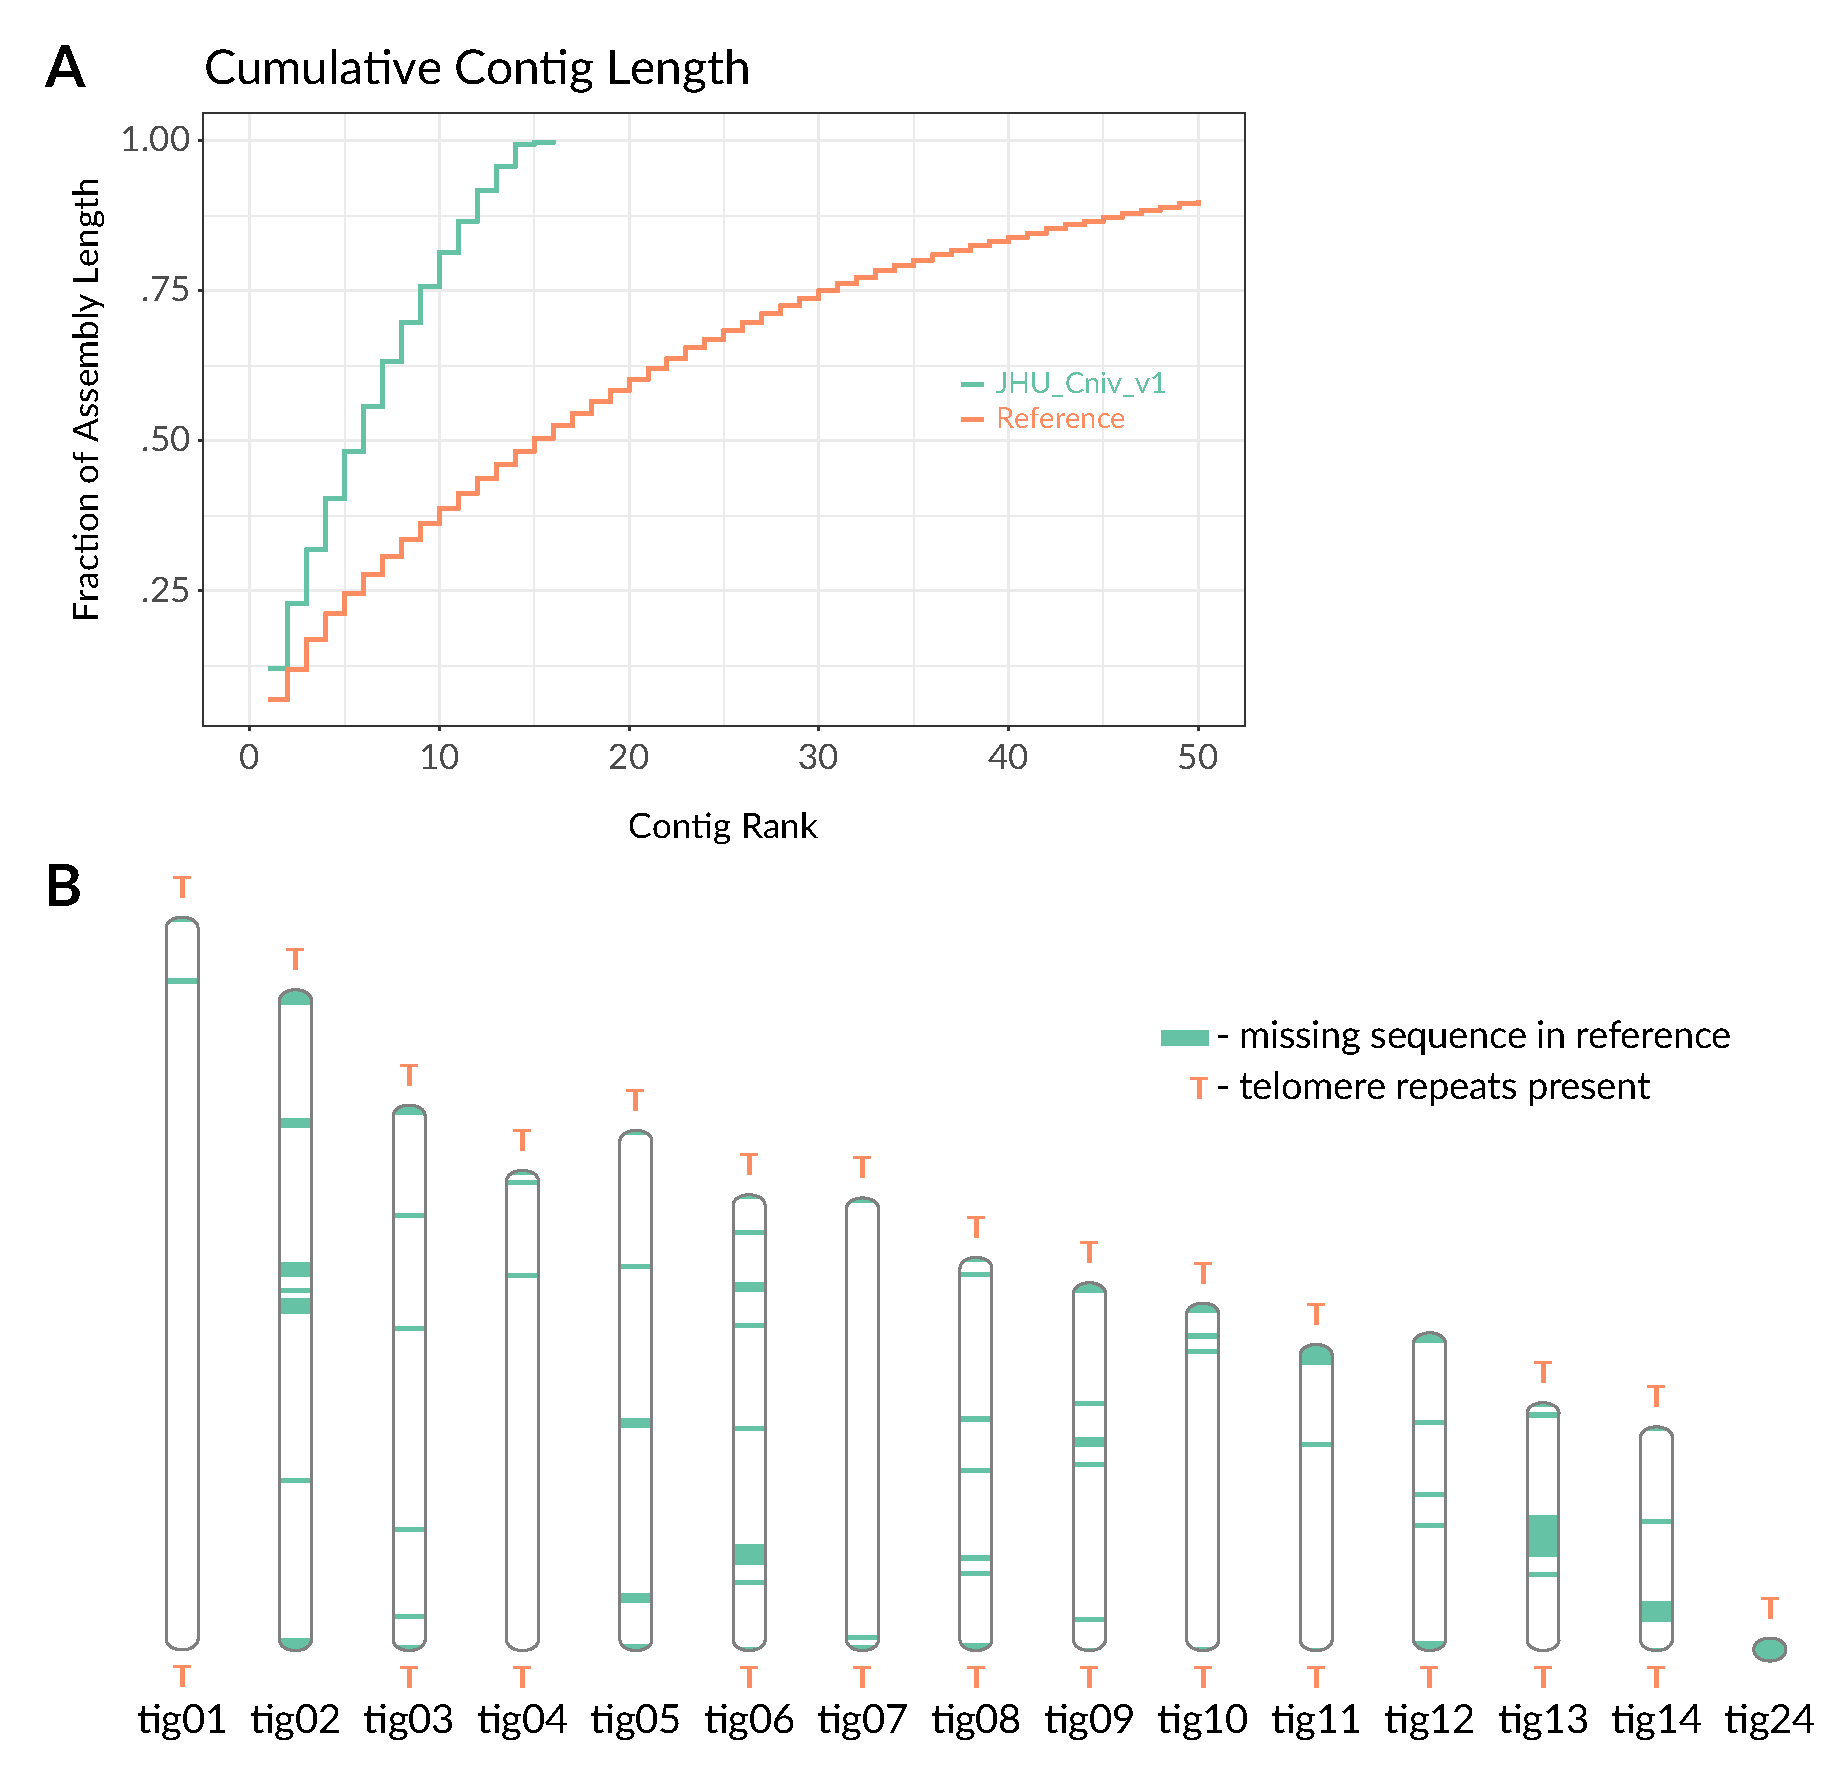
\includegraphics[width = 1\linewidth,keepaspectratio]{figure/asms.pdf}
\caption[Characteristics of the JHU\_Cniv\_v1 assembly]{{\bf Characteristics of the JHU\_Cniv\_v1 assembly.} {\bf (A)} Cumulative lengths of the 50 longest sequences in our assembly and previous reference genome. {\bf (B)} Ideogram of assembly. Sequence that is missing in the reference genome is shown along each non-mitochondrial contig, and the positions of telomere repeats are marked. }
\label{fig:asms}
\end{figure}


\begin{table}[!hb]
\centering
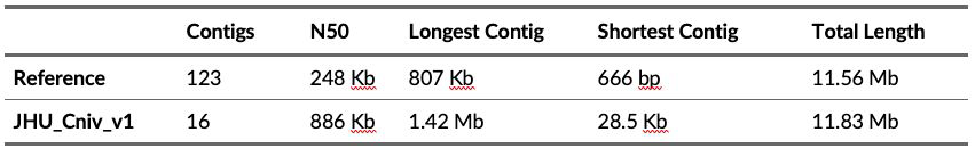
\includegraphics[width = 1\linewidth,keepaspectratio]{figure/asmstats.pdf}
\caption[Assembly Statistics]{{\bf Assembly Statistics.} Assembly statistics of JHU\_Cniv\_v1 and the reference genome for \textit{C. nivariensis}. }
\label{tab:asmstats}
\end{table}


To determine whether JHU\_Cniv\_v1 contigs represent full chromosomes, we looked for telomere repeats in our assembly and attempted to use related yeast reference genomes to scaffold. In our assembly, 11 contigs terminate at both ends in repeats of CTGGGTGCTGTGGGGT, the telomere sequence of \textit{Candida glabrata} \citep{McEachern1994-mf}. The other 4 non-mitochondrial sequences terminate only at one end in this telomeric repeat ({\bf Figure \ref{fig:asms}}, {\bf Table \ref{tab:telotable}}), suggesting they may scaffold to form two additional chromosomes. This suggests that, like \textit{C. glabrata}, the \textit{C. nivariensis} genome also contains 13 chromosomes.

\begin{table}[!ht]
\centering
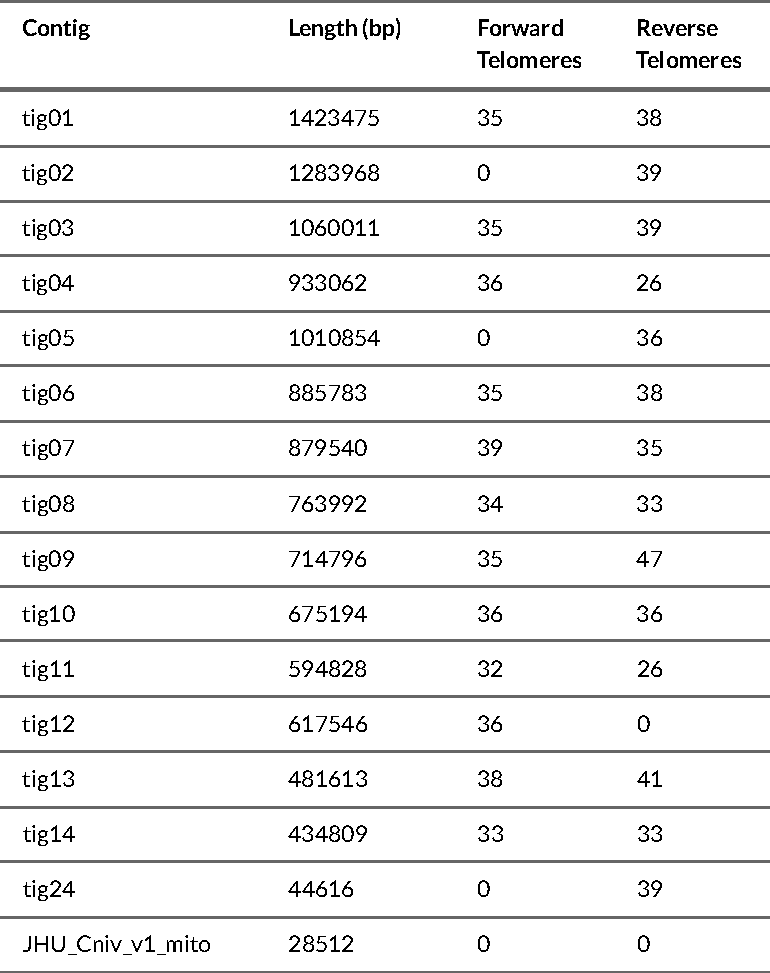
\includegraphics[width = .75\linewidth,keepaspectratio]{figure/telotable.pdf}
\caption[Contig and telomere lengths]{{\bf Contig and telomere lengths.} Contig lengths and the number of times the forward and reverse telomere sequence appears in each }
\label{tab:telotable}
\end{table}


We tried to further scaffold our assembly using the more contiguous and highly related \textit{glabrata} genome as a reference, but we found that reference based scaffolders such as Medusa v1.6 \citep{Bosi2015-rm} and RagTag v1.0.2 \citep{Alonge2019-re} either placed telomeric sequences in the middle of scaffolds or made no improvement ({\bf Figure \ref{fig:telopos}}). Upon aligning the \textit{C. glabrata} genome to JHU\_Cniv\_v1 using Mummer, we found only sporadic shared segments of negligible length ({\bf Figure \ref{fig:speciesmum}}), as opposed to a nearly perfect 1:1 alignment between JHU\_Cniv\_v1 and the current \textit{C. nivariensis} reference genome ({\bf Figure \ref{fig:mummer}}). This indicated that the \textit{C. glabrata} genome is not sufficiently similar to \textit{C. nivariensis} to use as a reference for contig scaffolding. Using the \textit{C. nivariensis} reference genome for scaffolding similarly results in erroneous placement of telomere repeats in the middle of scaffolds, or no change to our assembly. This is unsurprising, as the \textit{C. nivariensis} reference genome is so highly fragmented.


\begin{figure}[!ht]
\centering
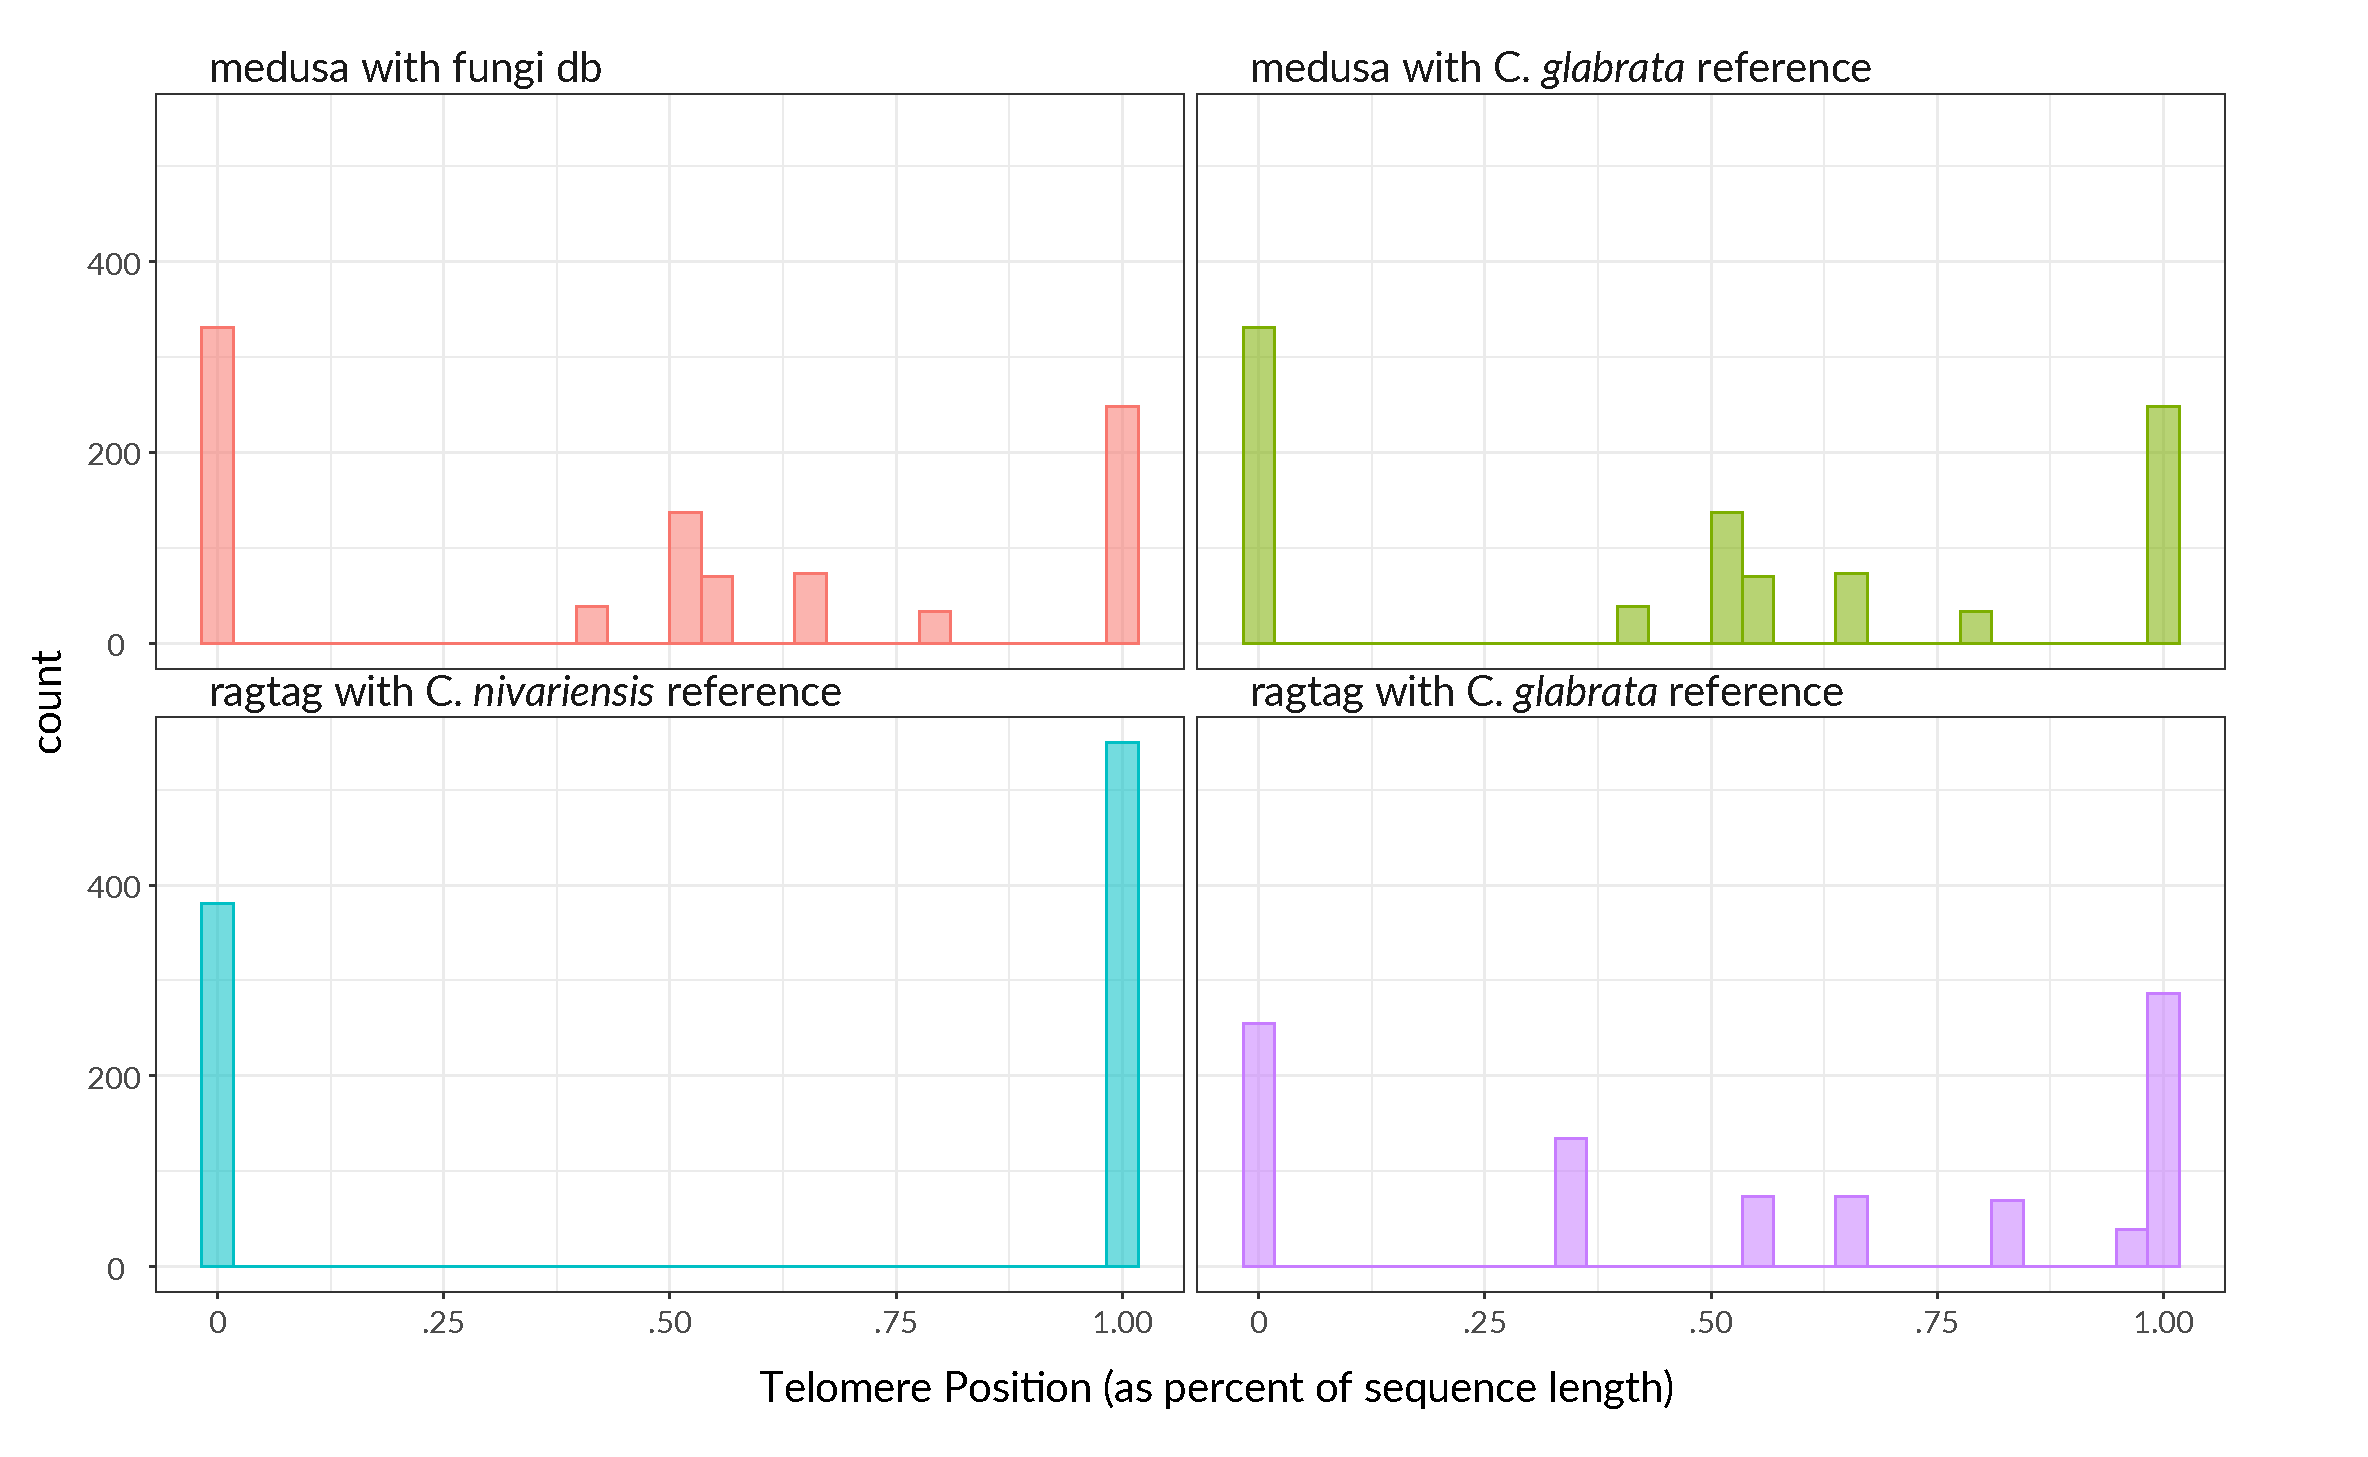
\includegraphics[width = 1\linewidth,keepaspectratio]{figure/telopos.pdf}
\caption[Telomere positions reference based scaffolds]{{\bf Telomere positions reference based scaffolds.} Histogram of telomere repeat positions in our assembly, and in scaffolds produced by RagTag and MeDuSa. When MeDuSa is used with a database including the reference genomes of \textit{C. nivariensis}, \textit{C. glabrata}, \textit{C. bracarensis}, and \textit{N. delphensis}, telomeres are placed in the middle of contigs. The same result is produced when only the \textit{C. glabrata} genome is used for scaffolding with MeDuSa, and MeDuSa fails to run when only the \textit{C. nivariensis} reference is used. When the \textit{C. nivariensis} reference genome is used for scaffolding with RagTag, no changes are made. When the more contiguous \textit{C. glabrata} genome is used with RagTag, telomere sequences are again placed in the middle of sequences, suggesting a scaffolding error. }
\label{fig:telopos}
\end{figure}



\begin{figure}[!ht]
\centering
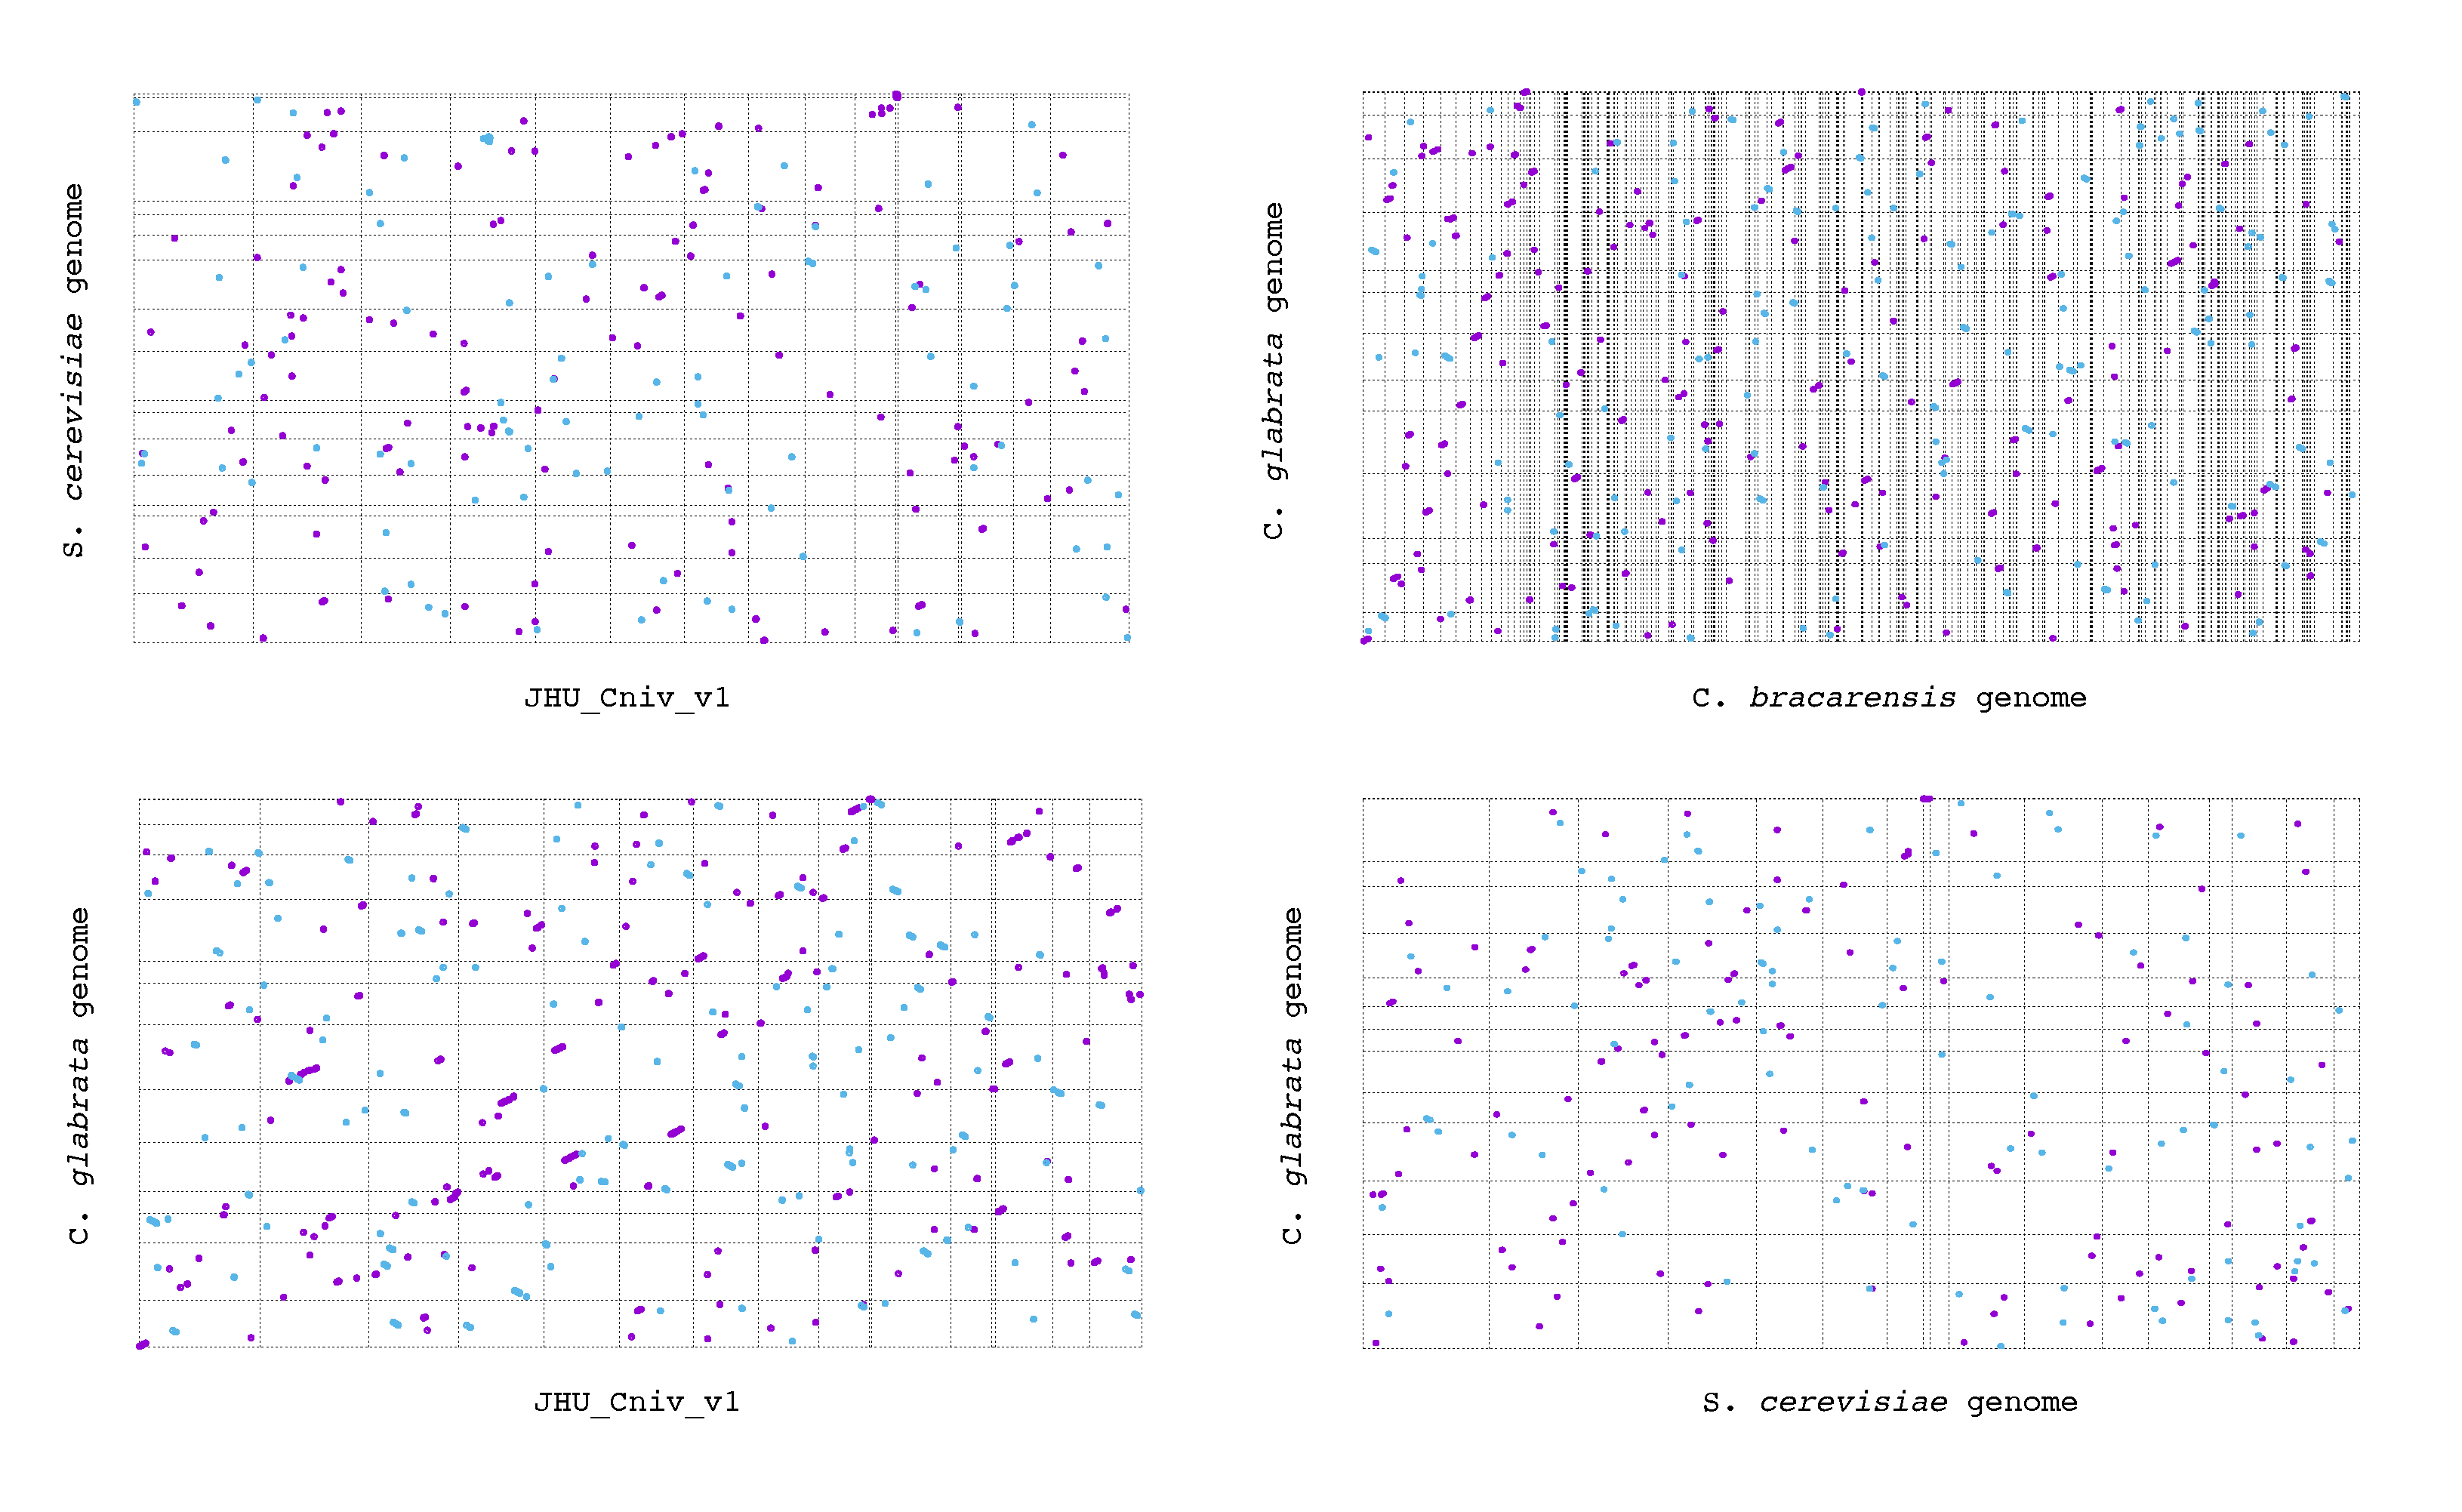
\includegraphics[width = 1\linewidth,keepaspectratio]{figure/speciesmum.pdf}
\caption[Whole genome alignments between related yeasts]{{\bf Whole genome alignments between related yeasts.} Whole genome alignment of our new assembly against the \textit{S. cerevisiae} (top left), and \textit{C. glabrata} (bottom left) reference genomes. For both, there are no long alignments, suggesting that there is little similarity in genome structure between these species and \textit{C. nivariensis}. \textit{C. bracarensis}, a close relative to both \textit{C. glabrata} and \textit{C. nivariensis}, also shares little genome similarity to \textit{C. glabrata} (top right), suggesting that yeast genomes within the \textit{glabrata} clade are not generally similar enough to support inter-species reference based scaffolding. We also compared \textit{C. glabrata} to the highly contiguous and complete \textit{S. cerevisiae} genome (bottom right) to check that genome contiguity alone did not bias the genome similarity detected. }
\label{fig:speciesmum}
\end{figure}



\begin{figure}[!ht]
\centering
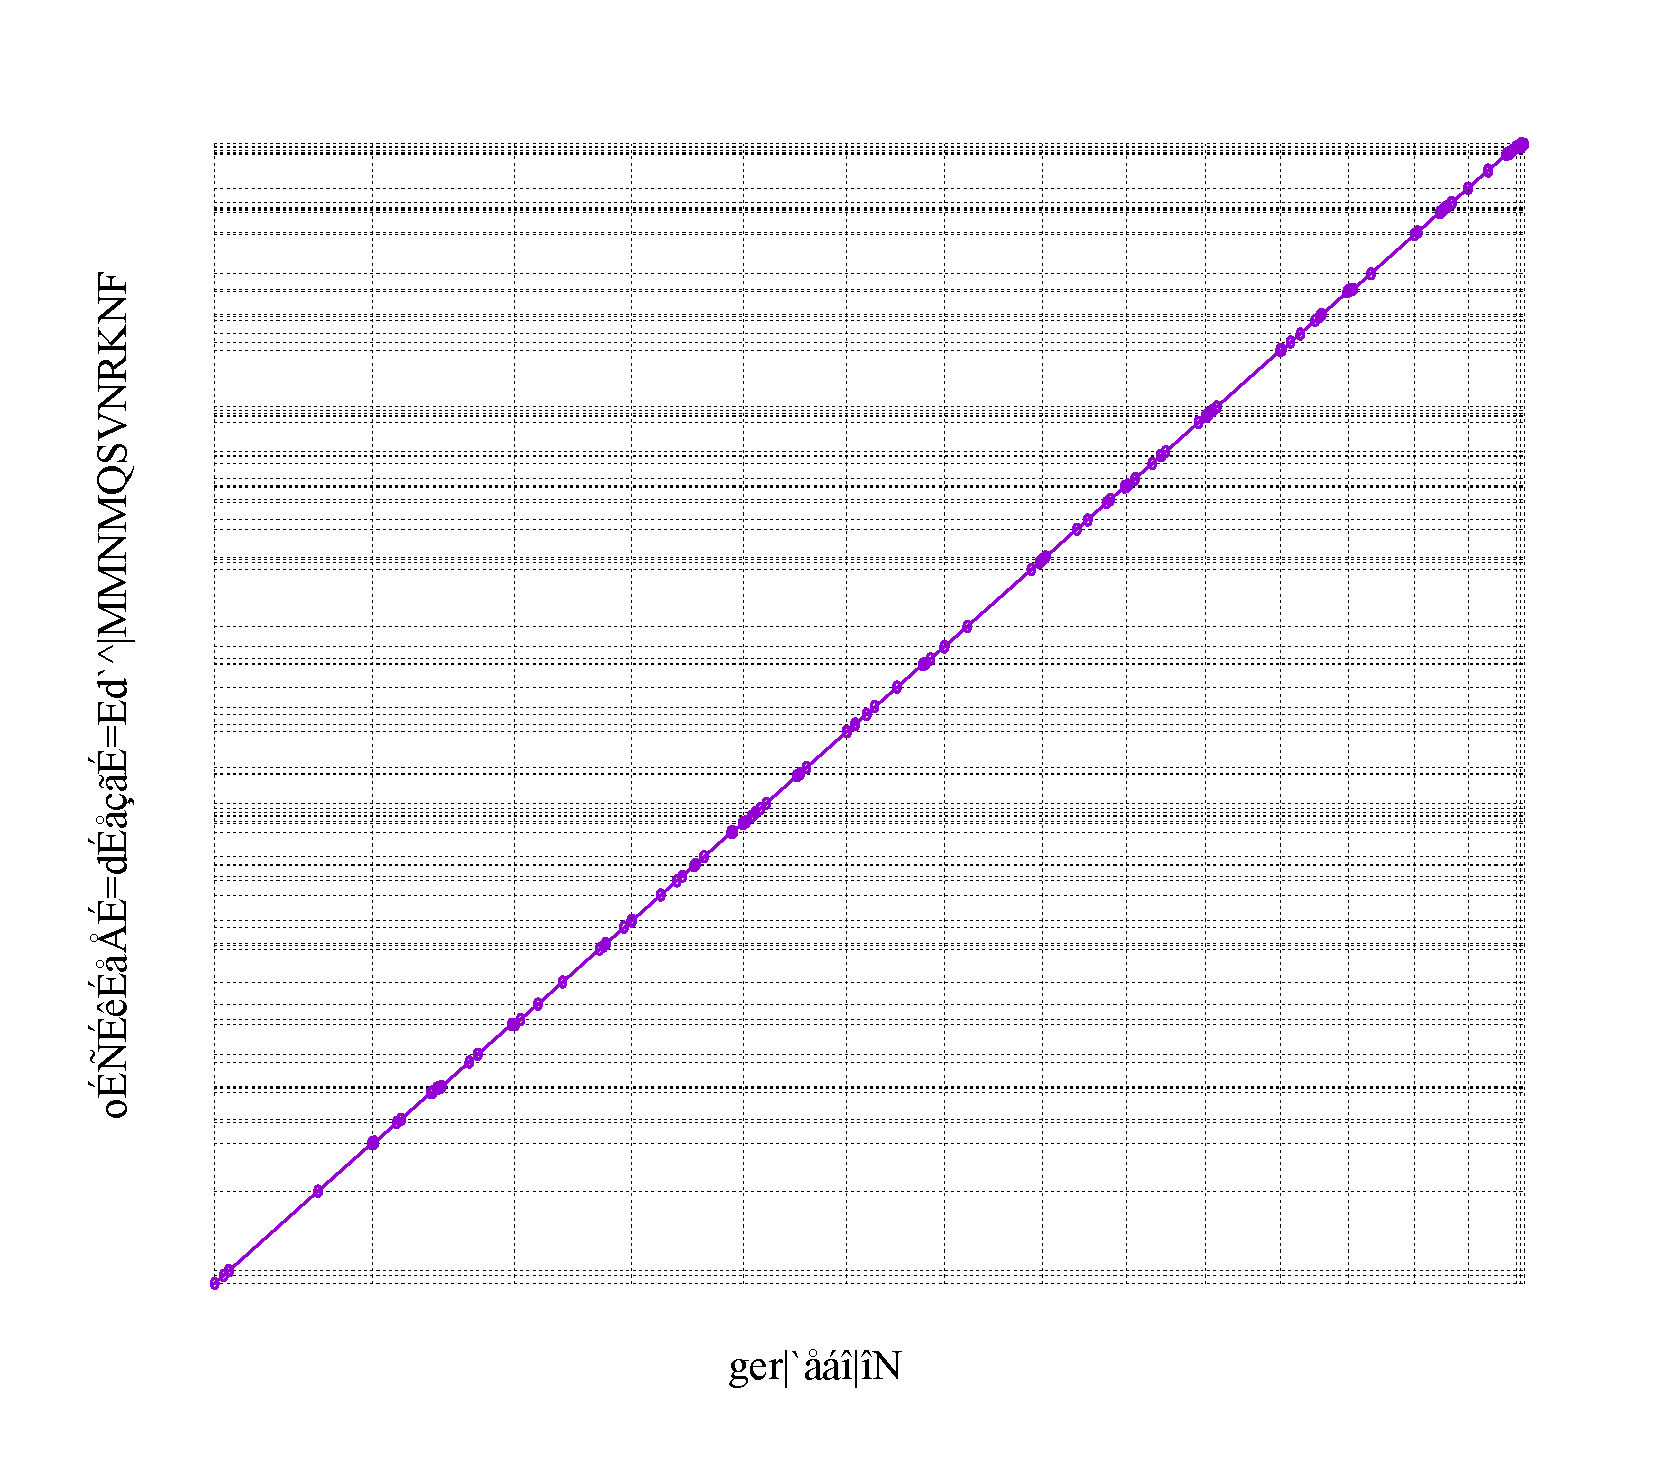
\includegraphics[width = 1\linewidth,keepaspectratio]{figure/mummer.pdf}
\caption[Whole genome alignment of JHU\_Cniv\_v1 and the \textit{C. nivariensis} reference genome]{{\bf Whole genome alignment of JHU\_Cniv\_v1 and the \textit{C. nivariensis} reference genome.} Whole genome alignment of the current reference genome (y axis) compared to our new assembly (x axis). Alignments match with no notable structural variants, and very little missing or duplicated sequence. }
\label{fig:mummer}
\end{figure}


\subsection{Genome completeness}
\label{sec:gencomp}

To assess assembly completeness, fungal single-copy orthologs were checked using BUSCO v5.0.0 \citep{Simao2015-zz} and its available saccharomycetes\_odb10 database. Out of 2137 BUSCOs searched, JHU\_Cniv\_v1 has only 14 missing, 13 of which are also missing in the current reference ({\bf Figure \ref{fig:busco}}). This additional missing gene, RNA polymerase archaeal subunit P/eukaryotic subunit RPABC4 (buscoID 41996at4891), though present in the reference, has the second lowest combined match length and match score among all genes searched. From the reference, we extracted the nucleotide sequence of this match using the coordinates reported by BUSCO, and searched for it in JHU\_Cniv\_v1 using BLAST. We found a full-length match with 99.9\% identity, suggesting that this BUSCO is not actually absent in JHU\_Cniv\_v1. Upon further examination of this alignment, we found that all seven nonmatching nucleotides consist of small deletions associated with poly-A or poly-T homopolymers, known error-prone regions for nanopore sequencing data \citep{Watson2019-tk}.

\begin{figure}[!ht]
\centering
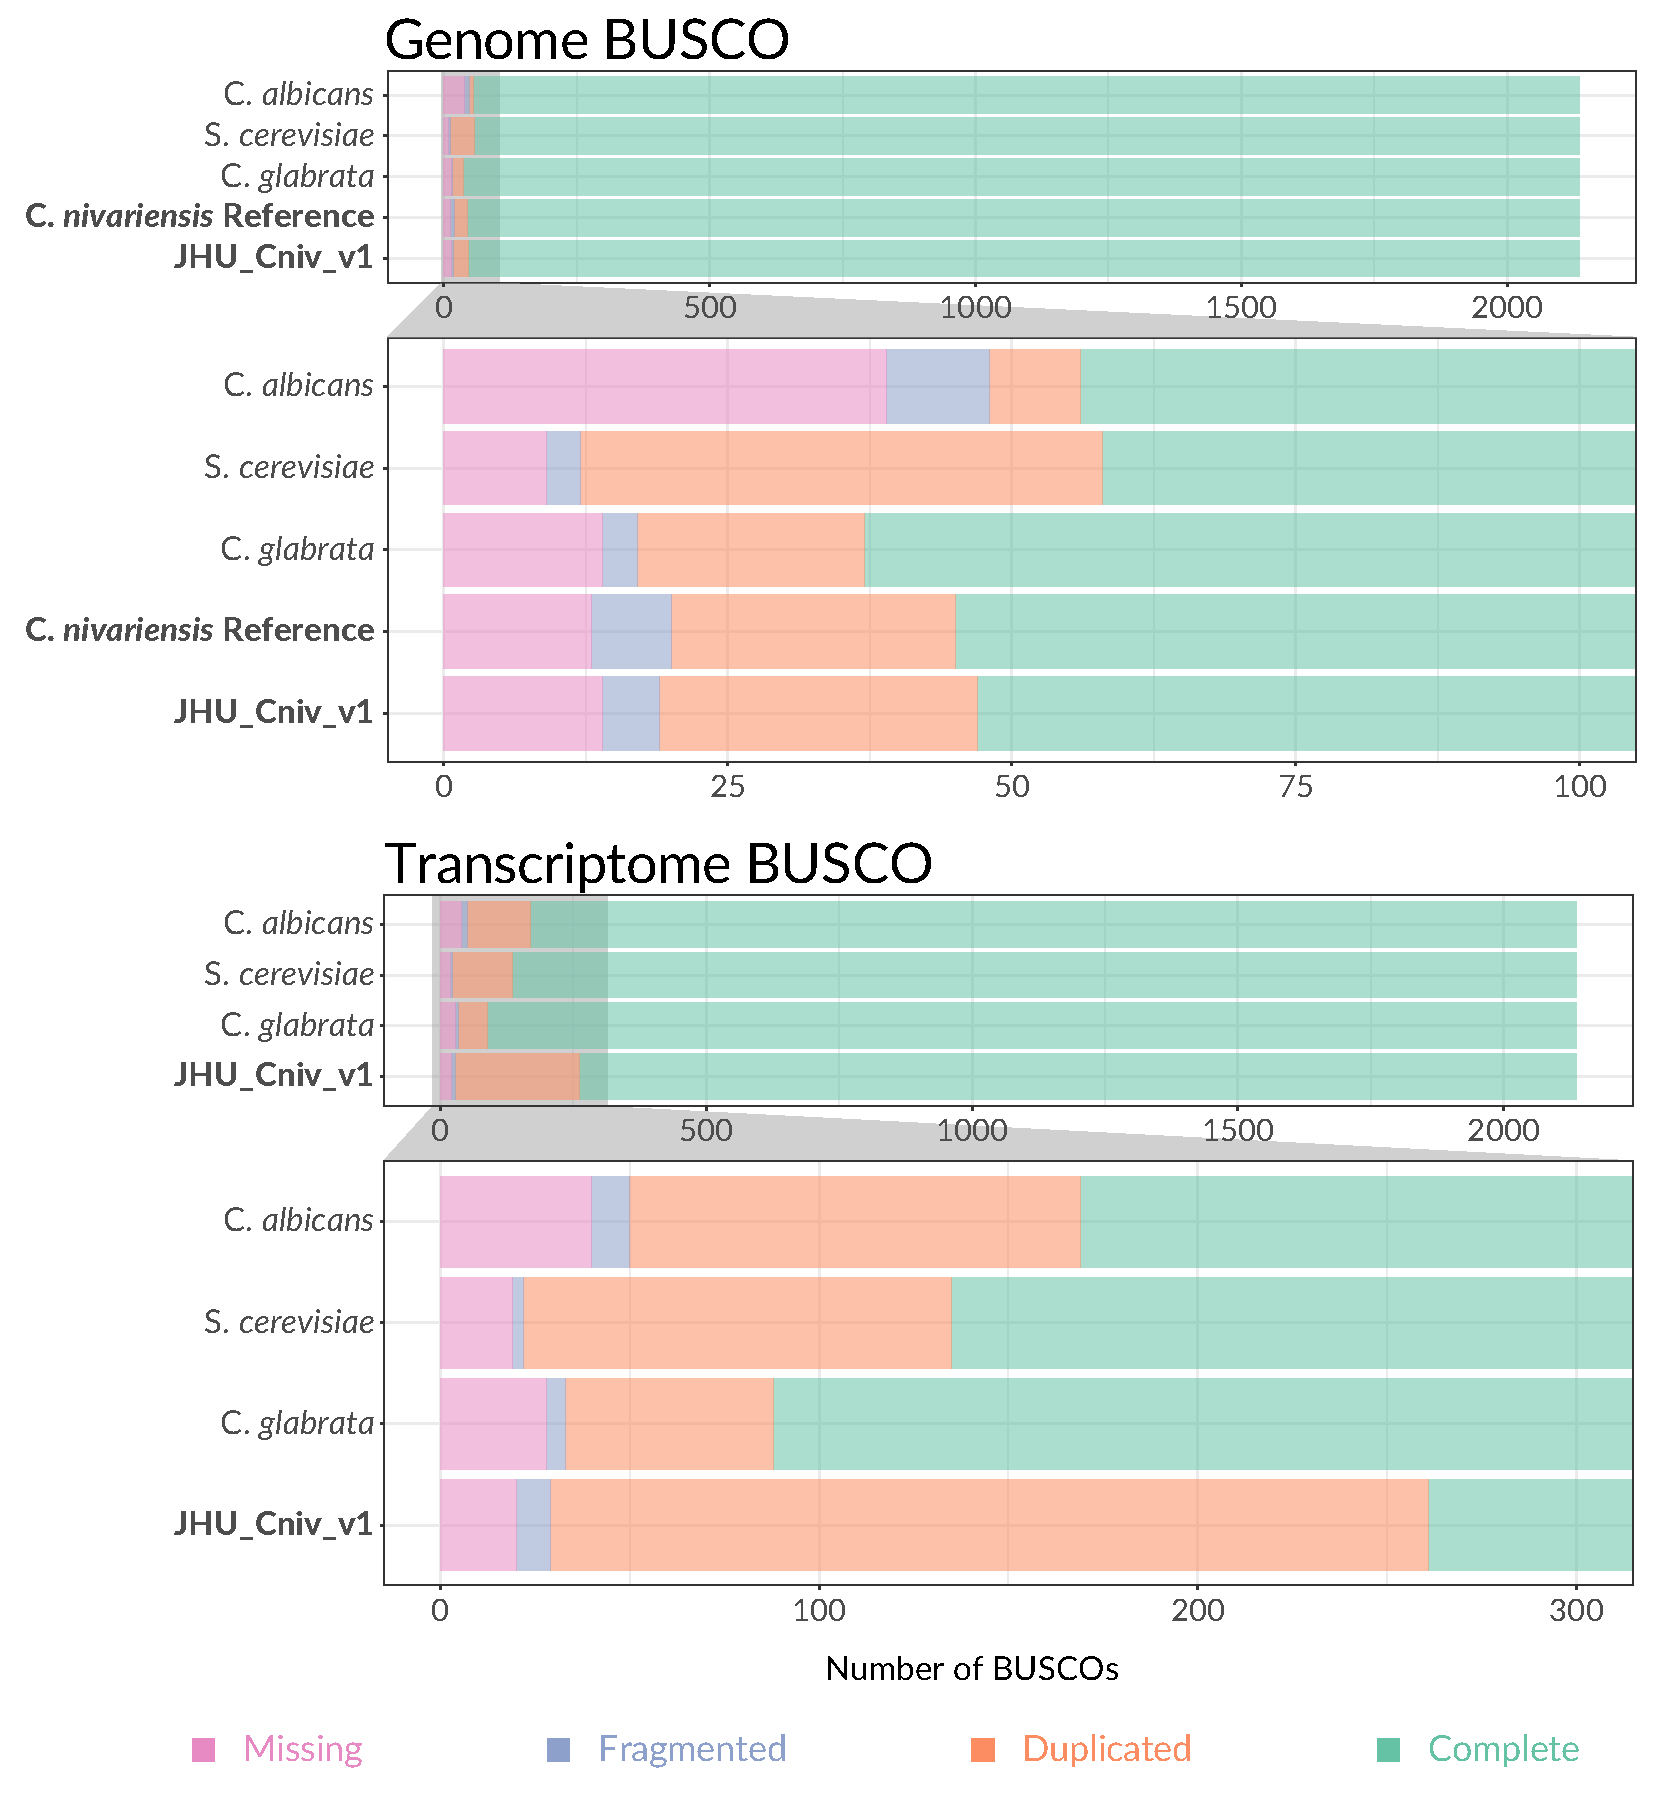
\includegraphics[width = 1\linewidth,keepaspectratio]{figure/busco.pdf}
\caption[Completeness of the JHU\_Cniv\_v1 assembly]{{\bf Completeness of the JHU\_Cniv\_v1 assembly.} Genome and transcriptome completeness Bar charts comparing BUSCOs detected in JHU\_Cniv\_v1 and accompanying transcriptome to those of the current \textit{C. albicans}, \textit{S. cerevisiae}, \textit{C. glabrata}, and \textit{C. nivariensis} reference genomes. No reference transcriptome is currently available for \textit{C. nivariensis}. }
\label{fig:busco}
\end{figure}


\subsection{Repetitive genes}
\label{sec:repgenes}


As \textit{C. glabrata} subtelomeric regions have been proven to be difficult to correctly assemble using short-read data \citep{Xu2020-ta}, we compare the copy number of \textit{C. glabrata} subtelomere gene homologs between the \textit{C. nivariensis} reference genome and JHU\_Cniv\_v1. Using the assembly and re-annotation of \textit{C. glabrata} from Xu et al. (2020), we extracted the sequences of the \textit{C. glabrata} subtelomere genes and used BLAST (v2.6.0+) to find any matches in the \textit{C. nivariensis} reference and JHU\_Cniv\_v1. We observed an identical set of 48 \textit{C. glabrata} subtelomere genes in both \textit{C. nivariensis} genomes but found that the copy number for several genes was greater in JHU\_Cniv\_v1 ({\bf Figure \ref{fig:gpicwps}}). To account for genes truncated by short contigs in the reference genome, we calculate copy number by summing the alignment lengths of all the hits of a particular gene and dividing by gene length. Of the 48 \textit{C. glabrata} genes with homology in \textit{C. nivariensis}, 35 are ribosomal. With the exception of just three ribosomal genes, which occur a similar number of times in both \textit{C. nivariensis} genomes, all homologous ribosomal genes appear once in the reference, and either four or six times in JHU\_Cniv\_v1 ({\bf Figure \ref{fig:gpicwps}}).

Using JHU\_Cniv\_v1, we identified GPI-anchored membrane proteins among annotated genes >1000-nt long. Using GffRead \citep{Pertea2020-lw}, we constructed the amino acid sequences for these genes and excluded any with internal stop codons. We then used PredGPI \citep{Pierleoni2008-aw} to predict which of these encoded GPI proteins, using an FDR cutoff of <0.0005 \citep{Xu2020-ta} to find 86 total genes. As GPI-anchored fungal adhesins typically contain tandem repeats \citep{Lipke2018-ow, Xu2020-ta}, we further filtered for genes overlapping with tandem repeats as classified by Tandem Repeat Finder and identified 53 of the GPI genes as putative adhesins. As with \textit{C. glabrata}, the putative adhesins typically spanned multiple kilobases ({\bf Figure \ref{fig:gpicwps}}), though we do not find very long (>13 kb) genes in contrast to several \textit{glabrata} GPI-CWPs. To find the corresponding adhesin genes in the \textit{C. nivariensis} reference genome, we again used BLAST, and compared the longest hit of each adhesin gene to the true length of the gene as predicted in JHU\_Cniv\_v1 ({\bf Figure \ref{fig:gpicwps}}). Notably, no hit in the reference genome exceeded 3.5 kb, and 27 of these adhesin genes are not found continuously, suggesting the previous reference either truncated or did not continuously assemble these important pathogenicity genes.


\begin{figure}[!hb]
\centering
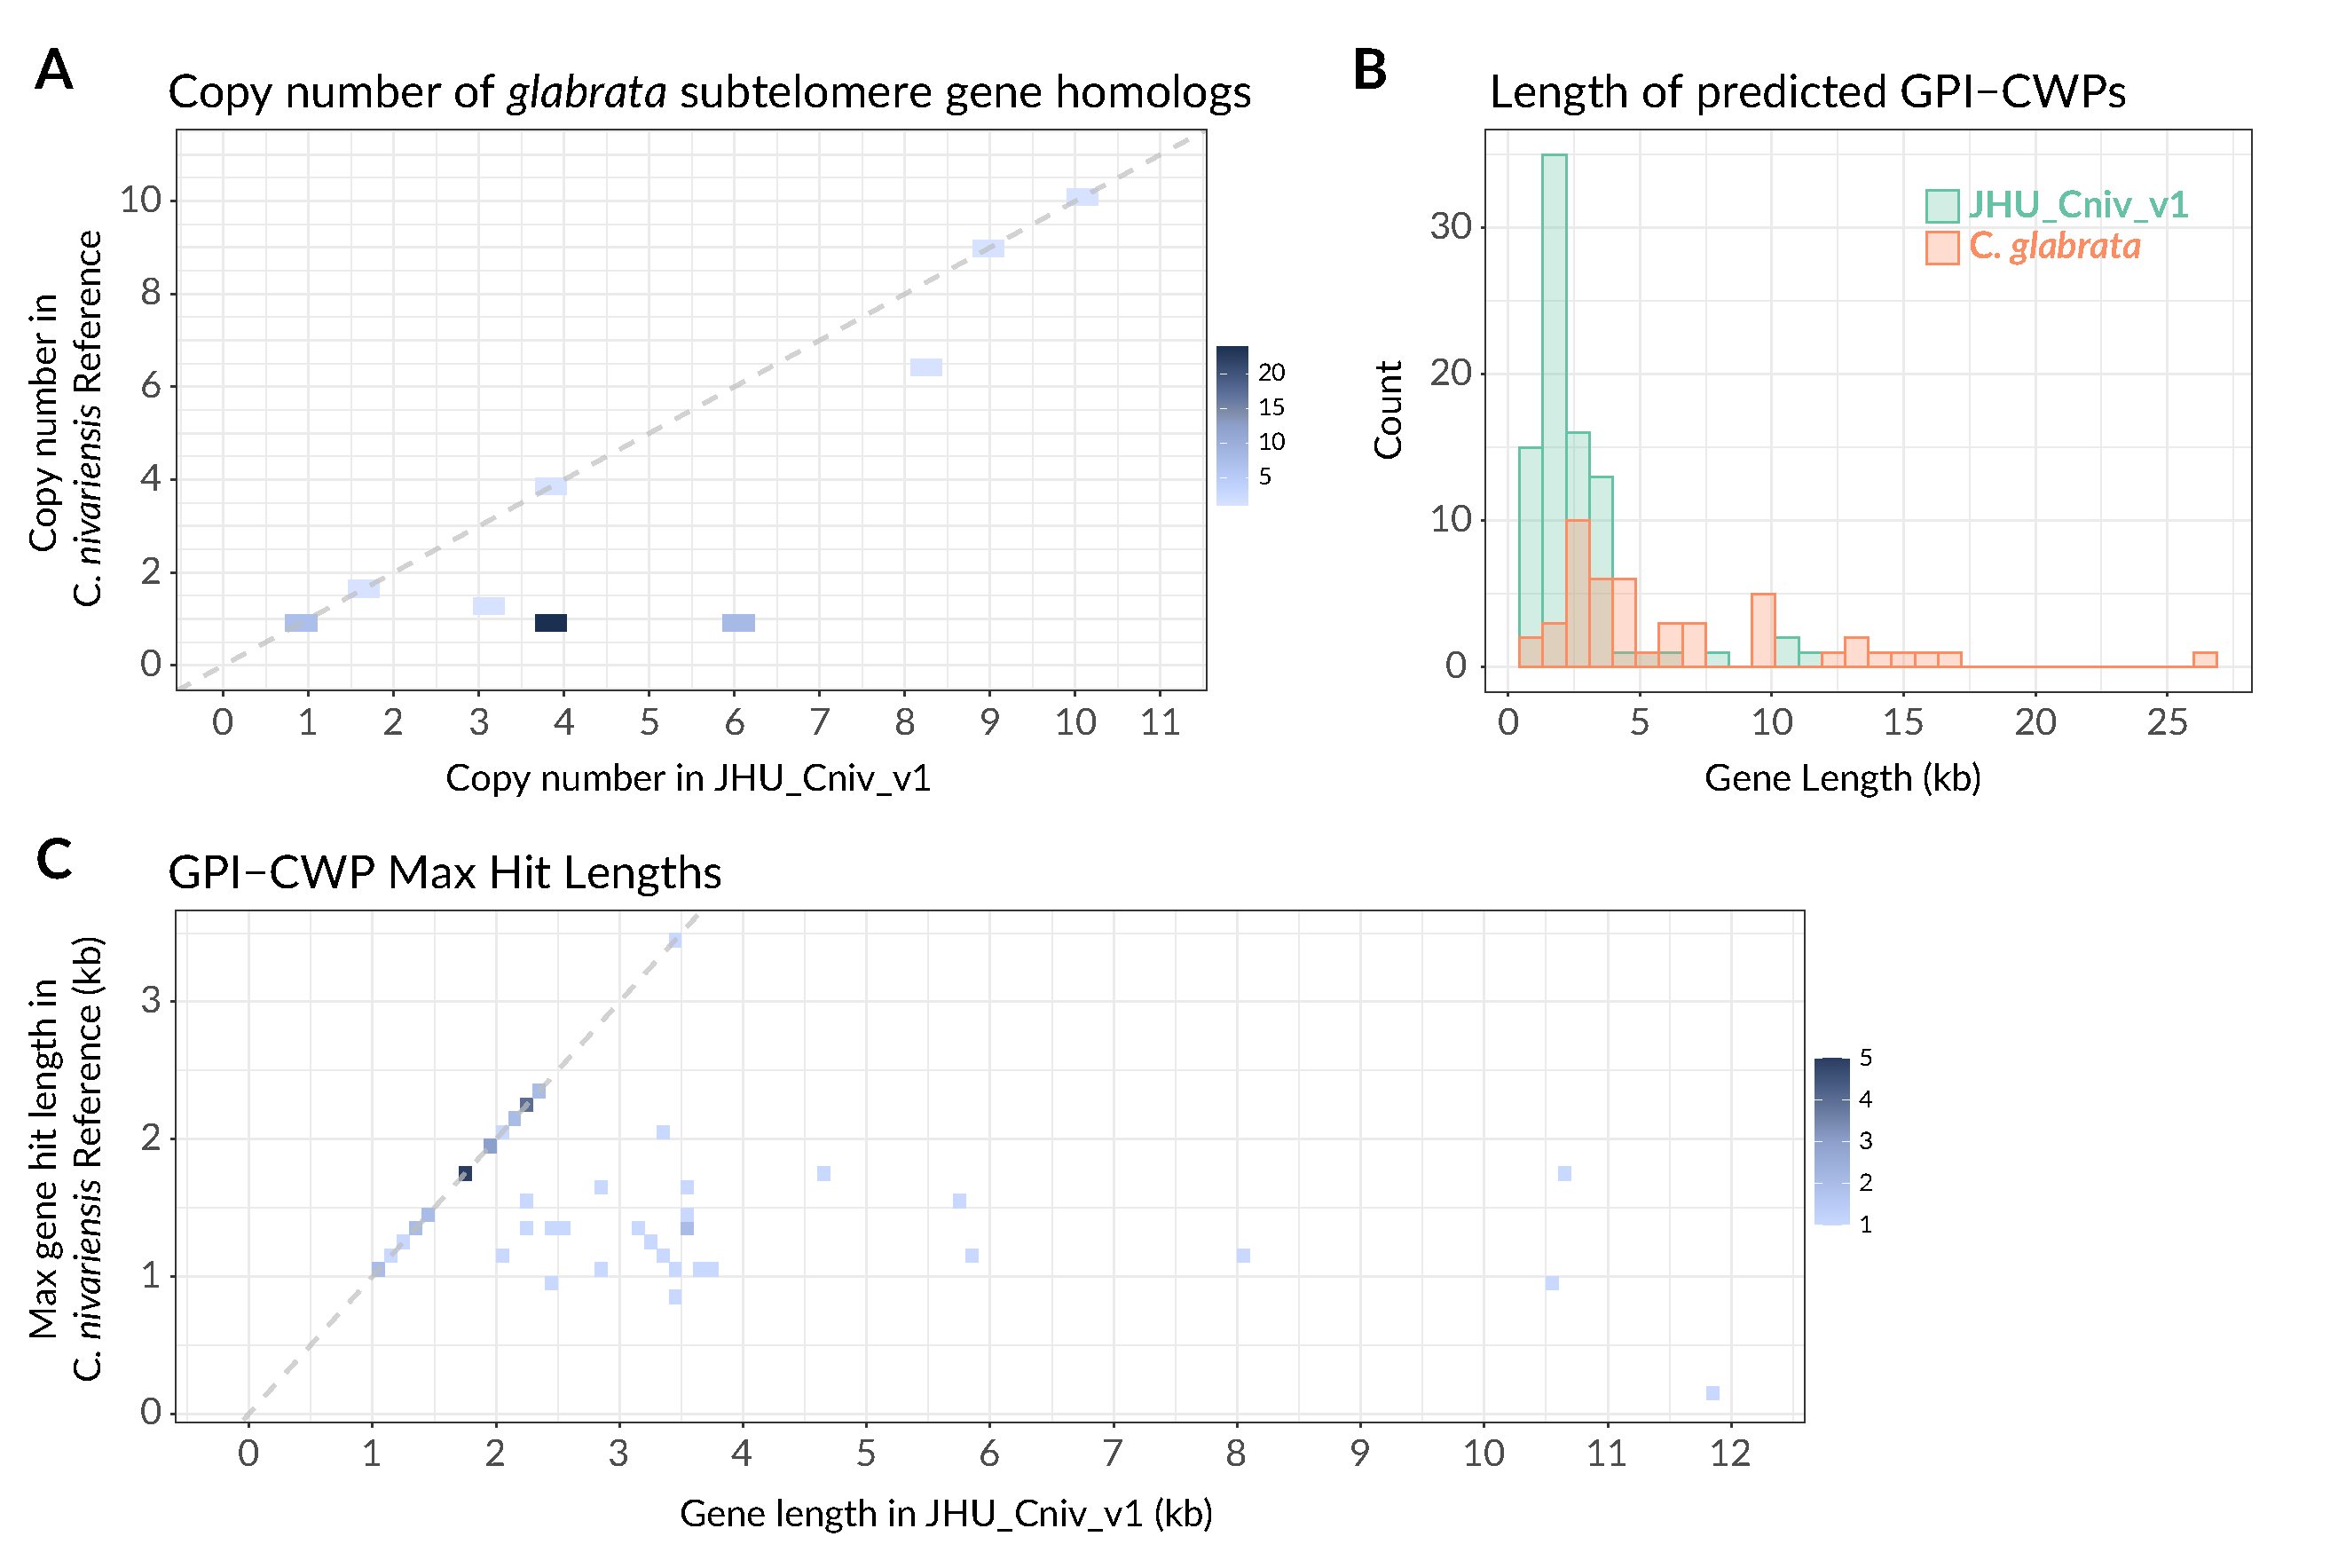
\includegraphics[width = 1\linewidth,keepaspectratio]{figure/gpicwps.pdf}
\caption[GPI genes]{{\bf GPI genes.} {\bf (A)} Scatterplot showing the number of times each glabrata subtelomere gene homolog appears in the \textit{C. nivariensis} reference genome and in JHU\_Cniv\_v1. Overlapping points are shown on the color scale, and the y=x line is shown in dashed gray. {\bf (B)} Histogram of adhesion protein lengths in glabrata as annotated by Xu et al., and the lengths of predicted adhesion proteins found in JHU\_Cniv\_v1. {\bf (C)} Scatterplot showing the maximum BLAST alignment lengths for each predicted nivariensis GPI gene in JHU\_Cniv\_v1 and the \textit{C. nivariensis} reference genome. Overlapping points are shown on the color scale, and the y=x line is shown in dashed gray. }
\label{fig:gpicwps}
\end{figure}


\section{Discussion}
\label{sec:discuss}

JHU\_Cniv\_v1 is a high quality, extremely contiguous assembly of \textit{Candida nivariensis} constructed by long reads and polished by short reads. It spans large, repetitive gaps in the \textit{nivariensis} genome that have fragmented short-read assemblies thus far, and includes a full mitochondrial chromosome, as well as telomere repeats. These telomere repeats are identical to those in \textit{C. glabrata} and have been found to be shared within the entire “\textit{glabrata} group” \citep{Gabaldon2013-bk}. The orientation of the telomeres suggests that \textit{C. nivariensis} has 13 chromosomes, which is in agreement with previous pulsed-field gel electrophoresis (PFGE) data \citep{Gabaldon2013-bk}. Furthermore, of the contigs missing telomere repeats on one end, we note that scaffolding tig05 with tig12 and tig02 with tig24 would result in 13 chromosomes that would all match PFGE length estimates to 8\% error or less, which is within the expected range of PFGE error for very large DNA fragments \citep{Cutting1988-mw}.

As assessed by BUSCO, genome completeness of the current \textit{C. nivariensis} reference and JHU\_Cniv\_v1 are comparable to other related yeasts, with our genome slightly improved over the previous reference. However, while JHU\_Cniv\_v1 is a much more contiguous assembly than any \textit{C. nivariensis} genome preceding it, the few remaining sequence errors still can pose a problem to downstream analyses, as evidenced by the seemingly absent BUSCO we manually identified.

Our accompanying RNA-seq data enabled us to annotate this genome, achieving a similar level of BUSCO completeness to some of the most highly studied model organisms. Our annotation has comparable or lower levels of missing and fragmented BUSCOs compared to the reference annotations, though more duplicated ones. While our annotation is largely comparable to those of similar yeasts ({\bf Table \ref{tab:refgenestable}}), it has not been manually curated, and should thus be treated as preliminary. Of course, as these organisms were grown under only one condition before RNA extraction, it remains unlikely that this annotation is fully complete.

\begin{table}[!ht]
\centering
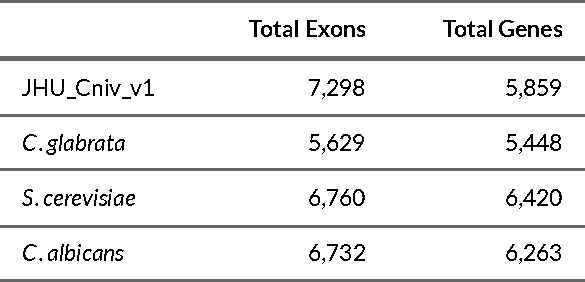
\includegraphics[width = .75\linewidth,keepaspectratio]{figure/refgenestable.pdf}
\caption[Gene and exon counts of JHU\_Cniv\_v1 and related yeasts]{{\bf Gene and exon counts of JHU\_Cniv\_v1 and related yeasts.} Gene and exon counts of our annotation and currently available reference annotations }
\label{tab:refgenestable}
\end{table}


To demonstrate the utility of genome and annotation contiguity, we examine genes from a difficult to assemble region in \textit{C. glabrata}. For each subtelomeric \textit{C. glabrata} gene with homology in \textit{C. nivariensis}, more copies were found in JHU\_Cniv\_v1, as its contiguity allows it to more easily capture repeated genome elements. We note that of subtelomeric \textit{glabrata} genes found, the majority are ribosomal, and of these, only three do not show a four or six times increased copy number in JHU\_Cniv\_v1. Due to the repetitive nature of rDNA arrays, it can be difficult for short-read genome assemblies to capture them in their full complexity. Conversely, our long-read assembly more easily spans these regions, potentially providing a clearer look at the biology in which they are involved.

In addition to genes arranged in complex and repetitive patterns, our more contiguous assembly enables analysis of large genes with internal repeats, such as GPI adhesins. Since these genes are so large, it can be difficult or impossible to predict them from fragmented assemblies which are unable to capture them in their full length. As adhesins are critical to understanding elements of pathogenicity in these yeasts, fragmented genome assemblies and missing gene annotations can be crippling to this dimension of research in these organisms.


\section{Methods}
\label{sec:methods}

\subsection{Media and growth conditions}
\label{sec:methods}

For genomic extractions, a single colony of \textit{C. nivariensis} CBS9983, originally isolated from a blood culture of a Spanish woman \citep{Alcoba-Florez2005-xn}, was inoculated into synthetic complete (SC) medium supplemented with 2\% glucose and shaken overnight at 30°C in a glass culture tube. For RNA extractions, \textit{C. nivariensis} CBS9983 was grown to log phase in SC medium supplemented with 2\% glucose at 30°C in a glass culture tube.

\subsection{DNA isolation and sequencing}
\label{sec:methods}

DNA was extracted from liquid culture using the Zymo Fungal/Bacterial DNA MiniPrep Kit according to manufacturer specifications. Two ONT sequencing libraries were prepared from the extracted DNA using the ONT rapid barcoding sequencing kit (SQK-RBK004), and each was sequenced on a separate MinION flowcell (R9.4). Two Illumina libraries were prepared with the Nextera Flex Library Prep Kit, each using 400 ng of extracted DNA. Both Illumina libraries were then sequenced on a single iSeq 100 run.

\subsection{RNA isolation and sequencing}
\label{sec:methods}

RNA was extracted from liquid culture using the Zymo Fungal/Bacterial RNA MiniPrep Kit. Using the NEBNext Poly(A) mRNA Magnetic Isolation Module, polyA tailed mRNA was isolated from the total RNA. Two ONT direct RNA sequencing libraries were prepared and sequenced on separate MinION flowcells, each using ∼200 ng of polyA selected RNA and the SQK-RNA002 sequencing kit. With the NEBNext Ultra II RNA First-Strand Synthesis Module and the NEBNext Ultra II Non-Directional RNA Second Strand Synthesis Module, cDNA was prepared from the isolated mRNA. Two individual Illumina libraries were then prepared with the Nextera Flex Library Prep Kit, each using 400 ng of cDNA. Both library replicates were then sequenced on a single iSeq 100 run, generating 2 × 150 paired-end reads.

\subsection{Genome assembly}
\label{sec:methods}

Nanopore data were basecalled using Guppy v3.2.4 on default settings. Reads greater than 3 kb long with an average basecalling quality score greater than 7 were assembled into 21 contigs using Canu v2.1 \citep{Koren2017-wf} on default settings with the genome size set to 11 m. Illumina DNA reads were trimmed for adapters and quality using Trimmomatic v0.39 \citep{Bolger2014-ax} using settings \texttt{LEADING:3 TRAILING:3 SLIDINGWINDOW:4:30 MINLEN:36}. The trimmed reads were then used to iteratively correct draft assembly using Freebayes v1.3.4-pre1 \citep{Garrison2012-iq} with alignments made by bwa mem v0.7.17-r1198-dirty \citep{Li2013-ec} using default settings. Changes were made at positions where both the alternative allele frequency was greater than 0.5 and the total number of alternate allele observations was greater than 5. We aligned and corrected the assembly iteratively for three rounds, after which further rounds of corrections made no changes.

Of our 21 corrected contigs, 5 were flagged as repeats by Canu and originally constructed from fewer than 180 nanopore reads. The remaining 16 contigs were constructed from over 1800 nanopore reads each. Because the five repetitive contigs were constructed from so few reads and were found to occur elsewhere in the assembly through Mummer v4.0.0rc1 \citep{Marcais2018-mm} and nanopore read alignment Minimap2 v2.17 \citep{Li2018-eq}, we excluded them from the final assembly. One 32-Kb contig was suggested to be circular by Canu, and therefore likely to be a mitochondrial sequence. To confirm, we aligned this contig to the complete mitochondrial genome of \textit{C. nivariensis} (NCBI: NC\_036379.1) using Mummer, and observed a 3662-bp sequence in the reference mitochondrial genome which appears at both ends of our 32-kb circular contig. Using the Mummer alignments ({\bf Figure \ref{fig:mito}}), we removed the extraneous 3662 bp from the end of our contig, resulting in a 28-kb mitochondrial genome, which we named “JHU\_Cniv\_v1\_mito.” Lastly, we remapped the ONT and Illumina reads back to the assembly, and found no bases with zero coverage, indicating that none of our contigs need to be further broken ({\bf Figure \ref{fig:covhist}}). Henceforth, we refer to this assembly as “JHU\_Cniv\_v1.”

\begin{figure}[!ht]
\centering
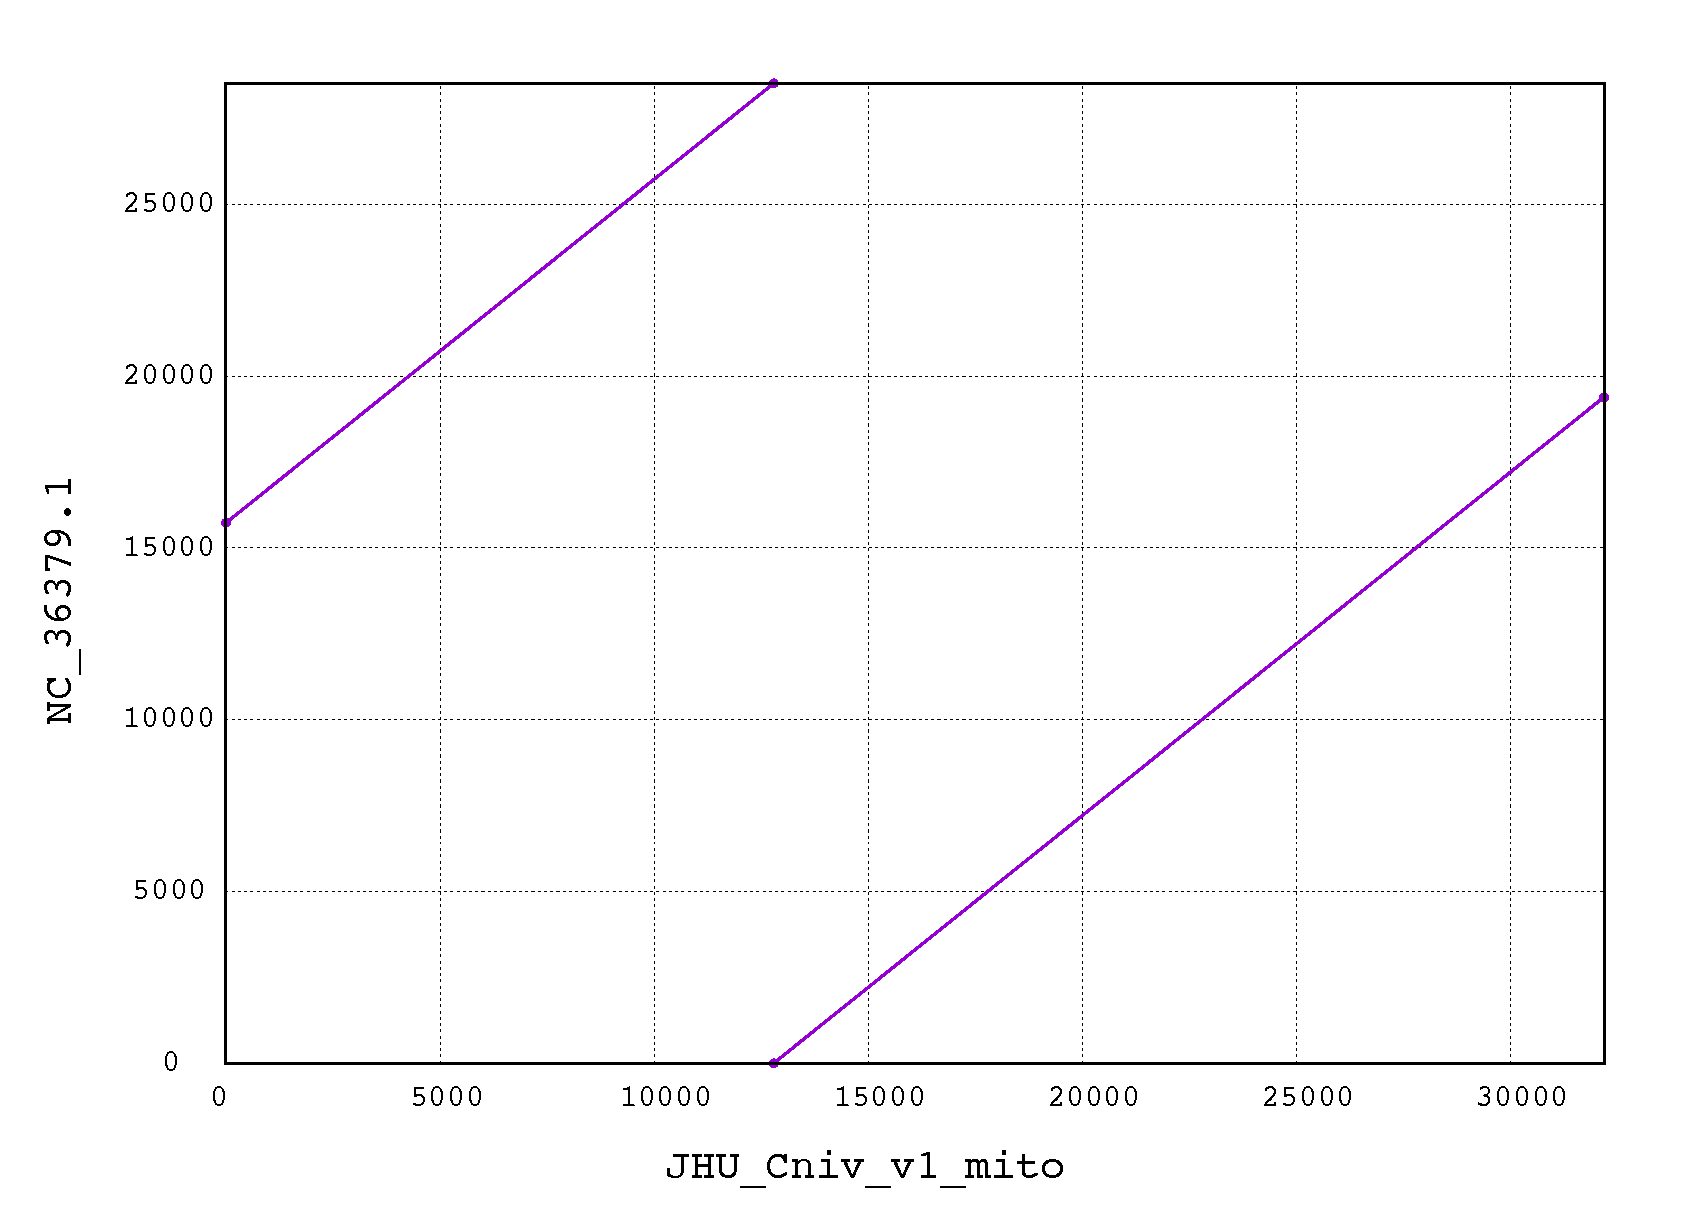
\includegraphics[width = 1\linewidth,keepaspectratio]{figure/mito.pdf}
\caption[Alignment of JHU\_Cniv\_v1 mitochrondrial contig and the \textit{C. nivariensis} mitochondrial genome]{{\bf Alignment of JHU\_Cniv\_v1 mitochrondrial contig and the \textit{C. nivariensis} mitochondrial genome.} Alignment of our 32Kb circular contig (x axis) with the completed mitochondrial genome of the \textit{C. nivariensis} reference genome (y axis). The final 3662bp of this contig appears twice in the reference genome. }
\label{fig:mito}
\end{figure}


\begin{figure}[!ht]
\centering
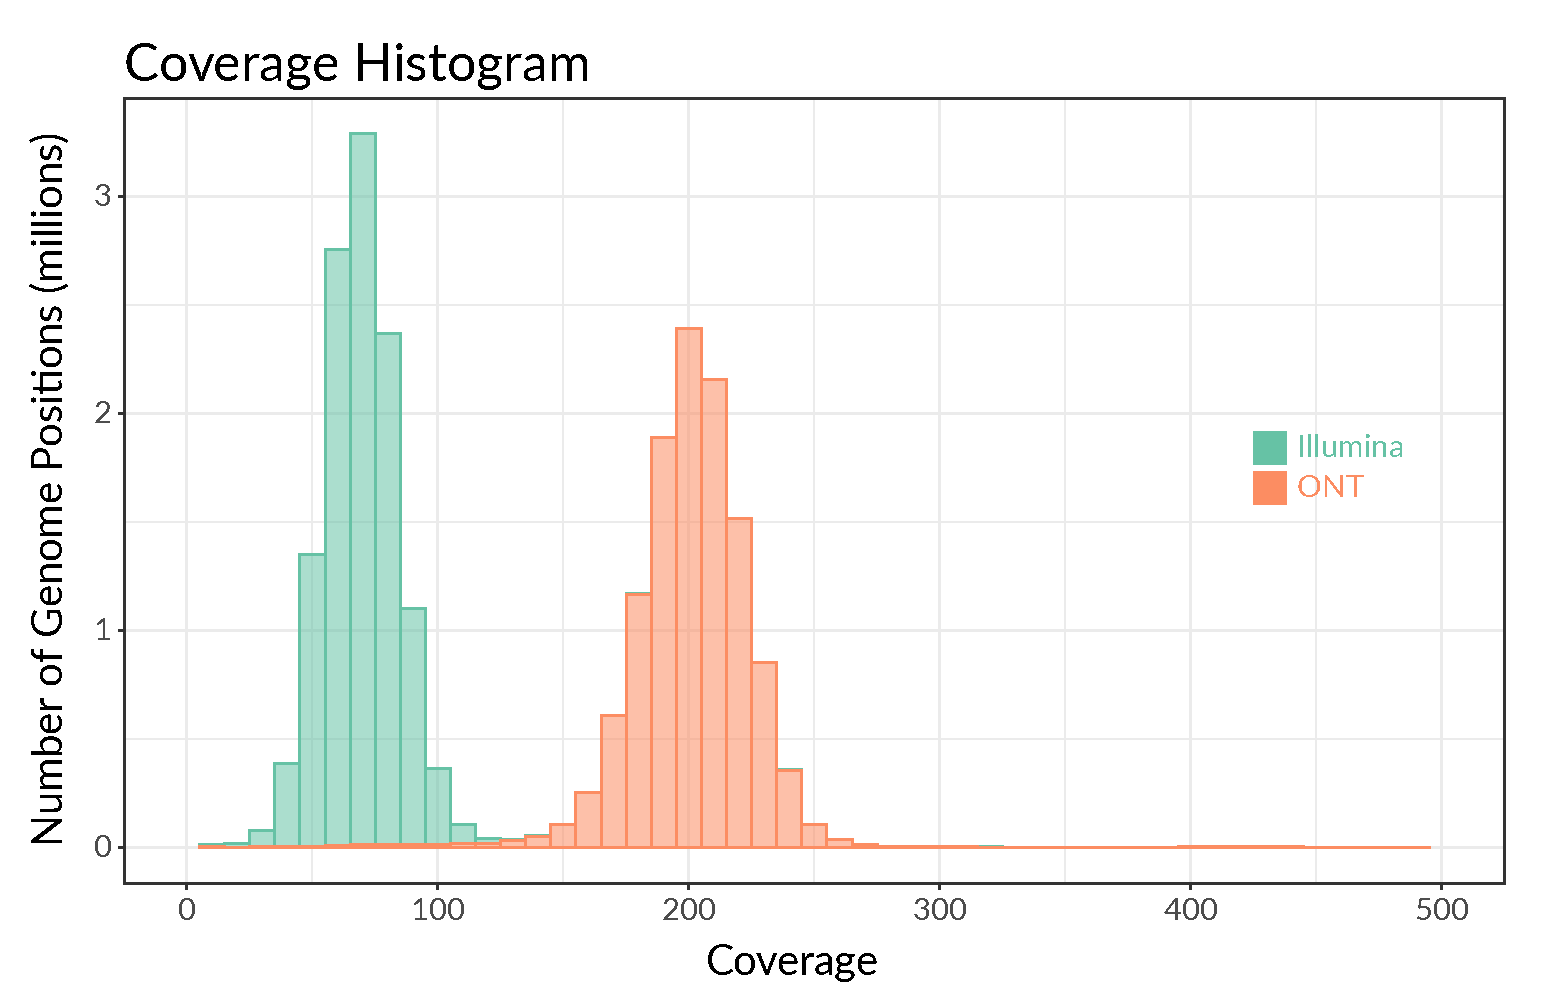
\includegraphics[width = 1\linewidth,keepaspectratio]{figure/covhist.pdf}
\caption[Coverage histograms]{{\bf Coverage histograms.} Histogram of coverage per base in our assembly by filtered (>3kb) ONT reads and trimmed Illumina reads. }
\label{fig:covhist}
\end{figure}


Repeat regions were identified by Tandem Repeats Finder v4.09 \citep{Benson1999-lr} with settings \citep{Xu2020-ta}: \texttt{match = 2, mismatch = 7, delta = 7, pm = 80, pi = 10, minscore = 50, maxperiod = 600}. Multimapping short reads were identified using bwa mem \citep{Li2013-ec} on default settings.

\subsection{Annotation}
\label{sec:methods}

Illumina RNA-seq reads were trimmed using Trimmomatic v0.39 \citep{Bolger2014-ax} in order to check for any remaining adapter sequences and to filter out reads with low base quality. HISAT2 v2.1.0 was used on default settings to align the trimmed cDNA reads to the assembly. The BRAKER v2.1.5 pipeline \citep{Hoff2019-rd} was then used to make gene predictions using these alignments. Currently, ONT dRNA compatibility with BRAKER is in development, and that data was thus not used for prediction. Instead, ONT dRNA reads were aligned to the genome assembly using Minimap2 on recommended settings for nanopore direct RNA reads (\texttt{-ax splice -uf -k14}). Transcripts were then assembled from the dRNA alignments using StringTie2 v2.1.5 \citep{Kovaka2019-lg} with the long read option (\texttt{-L}). Using Liftoff v1.5.0 \citep{Shumate2020-fo}, we lifted over the annotations from \textit{C. glabrata} (NCBI: GCF\_000002545.3), \textit{Saccharomyces cerevisiae} (NCBI: GCF\_000146045.2), \textit{Candida albicans} (NCBI: GCF\_000182965.3).

Starting with the BRAKER predictions, GffCompare v0.12.1 \citep{Pertea2020-lw} was used to add nonoverlapping annotations lifted from \textit{C. glabrata}, \textit{S. cerevisiae}, and \textit{C. albicans} in that order. Specifically, we add any annotation with class code “u” in the GffCompare .tmap outputs when comparing our list of genes with a list of potential genes to add, since these refer to intergenic regions devoid of any overlap or proximity to previous annotations. Finally, we compared and added nonredundant transcripts assembled by StringTie2 to the annotation using GffCompare.

\begin{table}[!ht]
\centering
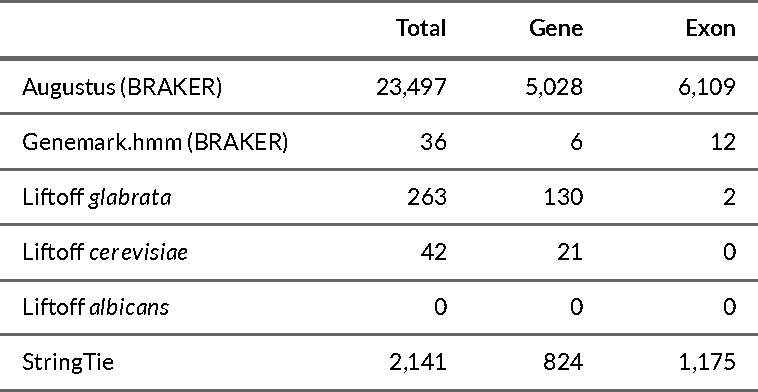
\includegraphics[width = .75\linewidth,keepaspectratio]{figure/genecounttable.pdf}
\caption[Contributions from each annotation software]{{\bf Contributions from each annotation software.} Number of genes and exons added by each software }
\label{tab:genecounttable}
\end{table}


\subsection{Data Availability}
\label{sec:methods}

All sequence data are available in the Sequence Read Archive, under BioProject PRJNA686979. This Whole Genome Shotgun project has been deposited at DDBJ/ENA/GenBank under the accession JAEVGP000000000. The version described in this here is version JAEVGP010000000. Code used for analysis is available at https://github.com/timplab/nivar.

\cleardoublepage
\printbibliography[title={References}]
\end{refsection}

\begin{refsection}[conclusion_chapter/conclusion_chapter.bib]
\chapter{Discussion and Conclusion}
\label{chap:conclusion}

As infectious diseases continue to be of growing interest and concern \citep{Baker2022-eb}, methods to monitor, diagnose, understand, and combat them must continue to evolve and improve. Sequencing technologies have developed at breakneck pace in recent decades \citep{Hu2021-dd, Schatz2013-vw}, and sequencing based investigative methods have been applied to great effect in almost all fields of biology and medicine. I have taken advantage of the unique properties of the most recent generation of sequencing technology for infectious disease applications, using it to identify and surveille AMR genes, assemble eukaryotic pathogen genomes, and link plasmids to hosts in complex microbial communities.

While nanopore sequencing can detect specific AMR genes quickly and agnostically \citep{Tamma2019-jg}, it can still be difficult to infer phenotypic resistance \citep{Yee2021-td}. Genomic data is able to provide information on an organism’s potential behavior, but observations of actual activity and function require transcriptomic or proteomic data. In situ functional studies of resistance mechanisms with metatranscriptomics could help to address these issues. As understanding of resistance mechanisms continues to grow, predictions of phenotypic resistance will become increasingly accurate and clinically actionable.

Use of long read sequencing for genome assembly has unlocked continuously larger genomes \citep{Neale2014-di}, and accompanying software has made high quality genome assembly more accessible than ever before \citep{Fan2021-cq}. As more and more eukaryotic pathogen genomes are sequenced, collated, and curated \citep{Aurrecoechea2017-tl}, they will become crucial to the development of sequencing-based diagnostics of infectious diseases \citep{Lu2018-wr}, in addition to being useful for furthering basic science research on these organisms.

Long-read data for metagenomic assembly not only produces longer contigs, but is able to preserve base modification data, which can be used for binning applications. Not only can contigs be grouped on the bases of base modifications, but reads can as well. Although this has not been shown using a single nanopore run, its possibility has been demonstrated using PacBio data \citep{Beaulaurier2018-mu}. Developing this capability in nanopore sequencing would enable multi-host plasmid assignments which are currently unfeasible.

\cleardoublepage
\printbibliography[title={References}]
\end{refsection}


% CV PDF file downloaded from the moderncv template available at Overleaf
% https://www.overleaf.com/latex/templates/modern-cv-and-cover-letter-2015-version/sttkgjcysttn#.Vw6PFRMrL65
\addcontentsline{toc}{chapter}{Curriculum Vitae} % CV must be in table of contents
\includepdf[pages={-}, pagecommand={}]{moderncv-2015.pdf} %continue page numbering through CV


\end{document}
